\chapter{Harmonics and electrons from plasma mirrors}
\label{Anticorrelated harmonic and electron emission from plasma mirrors}
\minitoc
\thispagestyle{empty}

\section{Review of electron acceleration mechanisms}\label{section:Review of electron acceleration mechanisms}

Electron acceleration mechanisms from solid-density plasma are highly dependent on the plasma scale length, intensity regime and pulse duration. Moreover, the notion of acceleration, or "heating", can designate electrons that remain inside the plasma or manage to "escape" from it. With nanosecond lasers for example, electron heating through inverse Bremsstrahlung due to collisions~\cite{schlessinger1979inverse,johnston1973correct} has to be taken into account to describe the formation of a hot-electrons population inside the plasma. When the plasma expands, the interaction with underdense regions is considerably increased. As a consequence, self modulation of the laser and filamentation appear, making the acceleration mechanism very complex~\cite{bach1983intensity}. It would be too ambitious to present an exhaustive list of the electron acceleration schemes based on solid-density targets. We will focus on acceleration schemes involving sub-picosecond to femtosecond laser interactions at relativistic intensities, essentially based on collisionless absorption mechanisms.\\


\noindent Interest for electron acceleration emerged with the need of collimated relativistic electron beams ($\sim$MeV) for fast ignition applications \cite{honrubia2006three}. Different acceleration mechanisms have been proposed to account for the production of fast electrons. We will give an overview of the different mechanisms found in the literature, which apply to planar solid targets (rather than cones, specific to fast ignition schemes) and highlight the specific experimental conditions in which they unfold.

\subsection{Resonant absorption}

We already described in section~\ref{sec:LaserAbsorptions} the principles of resonant absorption. Electron acceleration, or creation of a "hot-electron" population, is due a non-linear process called "plasma wave-breaking" occurring near the critical density~\cite{freidberg1972resonant,albritton1975cold}. In this model, the local plasma response around the critical density can be viewed, at a given time, as a phase wave which traps electrons and sweep them outwards, just like a surfer would catch a wave. However, this scheme is only valid for relatively long plasma scale length~($>\lambda$). 

\subsection{Vacuum heating}

The so-called "vacuum heating" mechanism occurs for short plasma scale length ($L << \lambda$) as opposed to resonant absorption. As exposed in~\cite{liseykina2015collisionless}, the term ``vacuum heating'' is not properly defined in the literature, and therefore two definitions emerge: (i) Vacuum heating is equivalent to the  "Brunel mechanism"(detailed description in section~\ref{section:Brunel absorption mechanism}) and designates electrons return to the plasma bulk~\cite{Brunel1987,Gibbon1992,Gibbon1994}; (ii) Vacuum heating is here again in reference to the "Brunel mechanism", but this time refers to electrons escaping into vacuum~\cite{chen2006surface,getz2005vacuum}.



\subsection{$J\times B$ heating}

We talk about $J\times B$ heating when the magnetic force is comparable to or even dominates the electric force $\sim e\g{E}$. This heating mechanism is counter-intuitive at first sight, because of the well known assessment that the magnetic force does not work, since $\delta W_{j\times B} = (J\times B) \g{v}dt= 0$. However, non averaged ponderomotive force (addressed in detail in section~\ref{section:Ponderomotive force and electron motion in vacuum}) is equivalent to the creation of $2\omega_0$ oscillating electric field~\cite{kruer1985j}. As a consequence, electrons undergo oscillations inside the plasma at twice the driving laser frequency~\cite{wilks1997absorption}. In this mechanism, electrons do not escape the plasma.
It is mostly efficient for low sub-critical densities ($\sim 10 n_c$) and its efficiency decreases exponentially with electron density~\cite{denavit1992absorption}, which means that it is suitable for very long gradient scale lengths. The experimental evidence of $j\times B$ electron heating was performed on very long plasmas ($\sim 40\,\mathrm{\mu m}$) by collecting the $2\omega_0$ radiation at the rear of a thin solid target~\cite{baton2003evidence} .




\subsection{Laser channel}


PIC simulations show that self-focusing or filamentation in near-critical plasmas is systematically associated with electron acceleration, up to $10-100\,\mathrm{MeV}$ for relativistic intensities \cite{askar1994magnetic,pukhov1996relativistic}. A model developed by Pukhov et al \cite{pukhov1999particle} confirmed by 3D PIC simulations states that when electrons are confined to a laser channel by quasi-static electromagnetic self-induced fields, they undergo betatron oscillations in  the direction of the laser polarization. When the betatron frequency equals that of the driving laser, a resonance occurs, generating electron bunches every laser period. Note that the plasma scale length involved in this mechanism is $L\sim 30\lambda$ in the direction of propagation $x$, at near-critical densities. The betatron frequency is given by the relation \cite{pukhov1999particle}:

\begin{equation}
\omega_{\beta}^2 = (\kappa_E + v_x \kappa_B)/\gamma
\end{equation}

\noindent resulting from the equation of motion being integrated for an electron moving in a electric field $E_y = \kappa_E y$ and a static magnetic field $B_z = -\kappa_B y$. 


\noindent Chen and al. \cite{chen2006surface} adapted this laser channel scheme to solid-density plasmas of scale length $L\sim 3\lambda$ and a laser intensity $a_0 \sim 2$ at grazing incidence $\theta_L = 70^{\circ}$ with respect to normal. The formation of quasistatic electromagnetic fields was attributed to the hot current due to $J\times B$ and vacuum heating.
The analytical approach is similar to that of Pukhov et a resonance occurs between the laser frequency and the betatron oscillations for:
\begin{equation}
\omega_{\beta} = \omega_0(1 - \sin(\theta_L))
\end{equation}

\noindent where $\omega_0$ is the laser frequency. This acceleration scheme shows similarities with plasmonic resonance, described hereafter.

\subsection{Surface plasmon resonance}

We already saw in section~\ref{subsection:Plasma perturbative approach} that a perturbed plasma resonates at the plasma frequency $\omega_p$ in response to a perturbation of its electron density. A semi-infinite plasma with a step like density profile is a resonator, which means that an emission line at frequency $\omega_p$ will be observed experimentally in the direction satisfying momentum conservation with the perturbation (photons, electrons for example). Ritchie et al. demonstrated in 1957 \cite{douglas1957excitation} that in addition to the bulk response of the vacuum / semi infinite plasma (or metals such as Aluminum or Gold), there exist proper surface modes that can also be excited, and therefore be detected experimentally in the emission spectrum either directly or through couplings with the driving laser, like Fano resonances for instance. These oscillation modes, called plasmons, are a consequence of Maxwell's continuity-equations at an interface between two media of respective permittivity $\epsilon_m$ and $\epsilon_d$. The plasmon wave vector in the plane defined by the interface is given by the relation:

\begin{equation}
k_{SP} = \frac{\omega}{c}\sqrt{\frac{\epsilon_m\epsilon_d}{\epsilon_m+\epsilon_d}}
\end{equation}

Note that the tangential component of the field in both media is implicitly supposed not equal to zero. This means that a laser undergoing perfect reflection on a plane surface does not generate plasmons because $E_{\parallel}(0^{+}) = 0$ by symmetry, but a surface with local defects, partially absorbing the light, breaks this symmetry and can give rise to plasmonic effects. In particular, plasmon-photon coupling on metallic coated gratings (where absorption is also possible) have been extensively investigated \cite{ritchie1968surface}.
Some research groups have demonstrated that it is possible to enhance the magnitude of surface plasmons at an interface by choosing the right incident angle for the driving laser \cite{fedeli2015electron}.

\begin{equation}
\frac{\omega}{c}\sin(\theta_L) + \frac{n\pi}{d} = k_{SP}(\omega)
\end{equation}

where $d$ is the grating period, $\omega$ the laser frequency and $n\in \mathbb{Z}$ the enhancement order. Experimental evidence of plasmonic enhancement has been achieved with relativistic-intensity fs laser pulses on structured plasma targets to accelerate protons \cite{ceccotti2013evidence} and electrons\cite{fedeli2015electron}: particles confined by the plasmonic magnetic field near the surface are accelerated "for a longer time" than in the case a planar surface by the purely electrostatic plasmonic potential. As a result, they gain more energy in the direction defined by vector $k_{SP}$ (i.e. parallel to the target surface).

\subsection{Stochastic heating}

Rigorously, a stochastic system is a system that cannot be described other than through a probability density function on a large number of particles. In the case of electron acceleration, electrons undergo stochastic (or chaotic) motion when they can no longer be described by well defined orbitals, or in other words, for an arbitrarily small perturbation of their initial position or canonical momentum, their trajectories in time can be radically different. \\
\noindent The observation of stochastic electronic motion in interference fields is a well-known topic. For instance, in the case of two counterpropagating laser pulses (plane waves) \cite{sheng2002stochastic} the final temperature of the electrons can exceed that predicted by the laser ponderomotive potential in a near critical density plasma medium by a factor close to 5. Other authors have shown multiwave systems could easily lead to suprathermal electrons because of stochastic heating \cite{mendonca1982stochasticity}.  The mechanism they described is an extension of wakefield acceleration schemes and consists in plotting the orbital solutions of the Hamiltonian corresponding to two counter-propagating lasers. For relativistic intensities, the motion is dominated by stochastic motion and the stable orbits are shifted to higher energy zones.

%The motion of a charge in a monochromatic linearly polarized plane wave is very well known and has been treated in numerous academic books \cite{LandauLip}. The solution in a plane were the electron is on average not moving  is a trajectory following an $8$ in the plane orthogonal to the propagation and symetric with respect to the polarization direction. 
%
%A convenient way to represent the appearence of a chaotic behavior is to make use of poincare sections. To generate a Poincare section in a conventional dynamical problem where the particle trajectories are known, one needs to choose a plane in real space,  and each time the trajectory $x(t)$ of a particle intersects that plane, the value $(x,\dot{x})$ is saved. After a infinite time, the Poincare map can be plotted using all the saved points as represented in Fig~\ref{Fig:PoincareSectionIllustration}. Using this method, we can visualize the apperance of chaos by a random repartitions of points in the poincare section.
%
%
%\begin{figure}[H]
%\begin{center}
%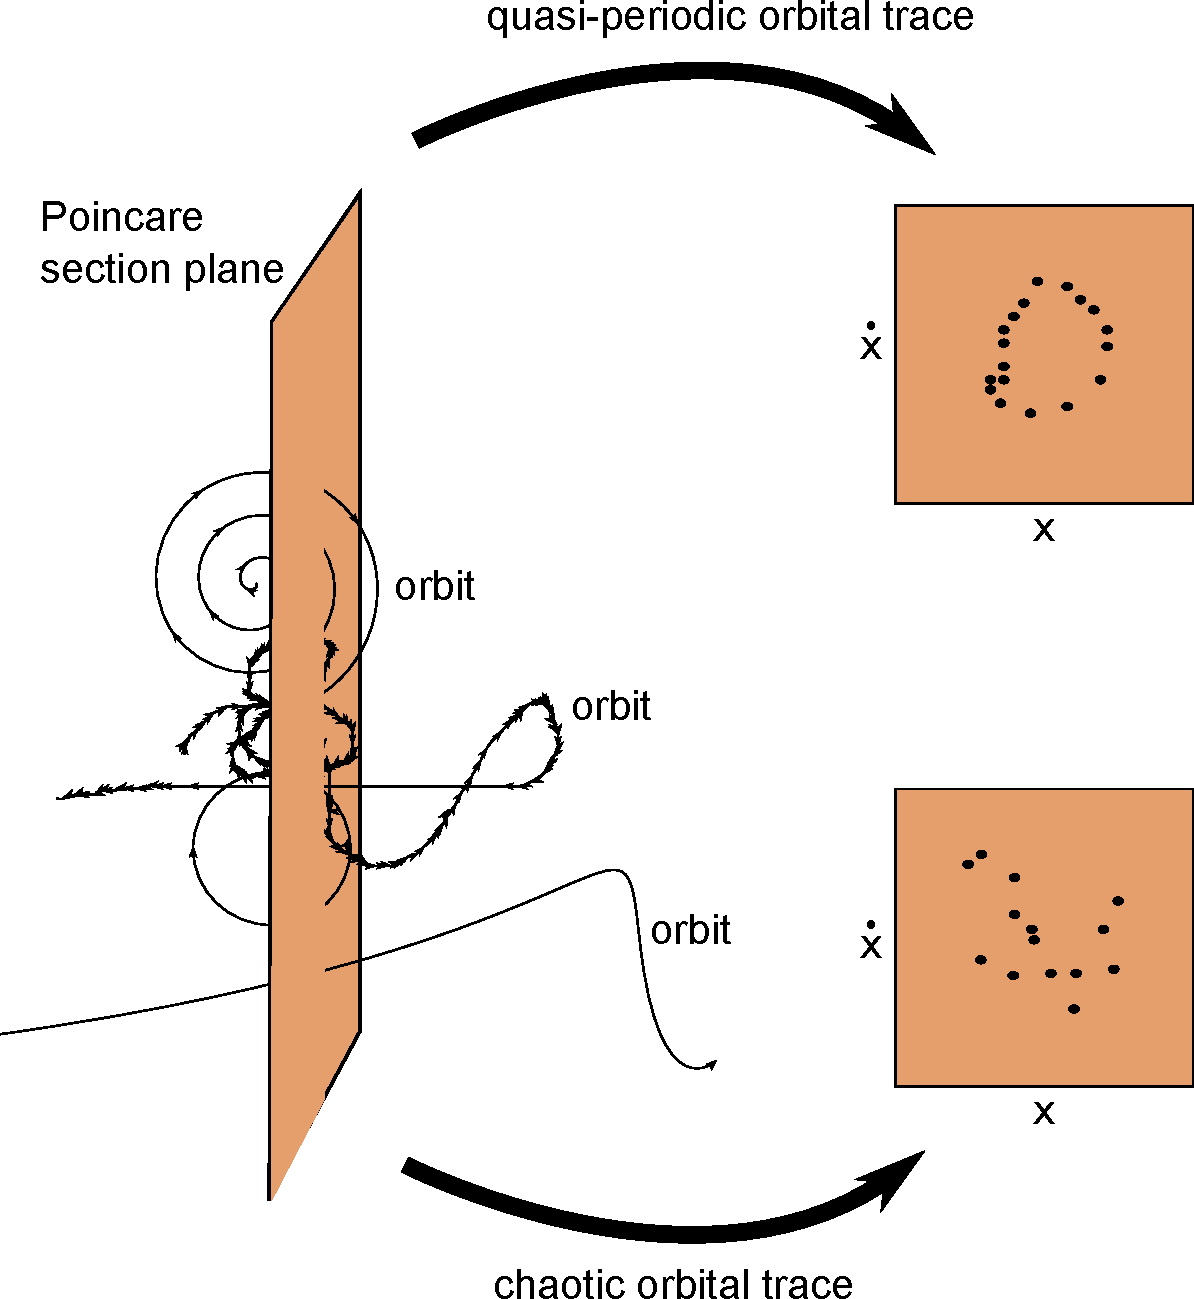
\includegraphics[width =8cm]{../chapitre2/images/PoincareSectionIllustration.pdf}$
%\caption{\label{Fig:PoincareSectionIllustration}Schematic representation of Poincare sections generated for 2 orbitals (quasi-periodic and chaotic)}
%\end{center}
%\end{figure}
%
%\begin{figure}[H]
%\makebox[\textwidth][c]{
%\begin{tabular}{cc}    
%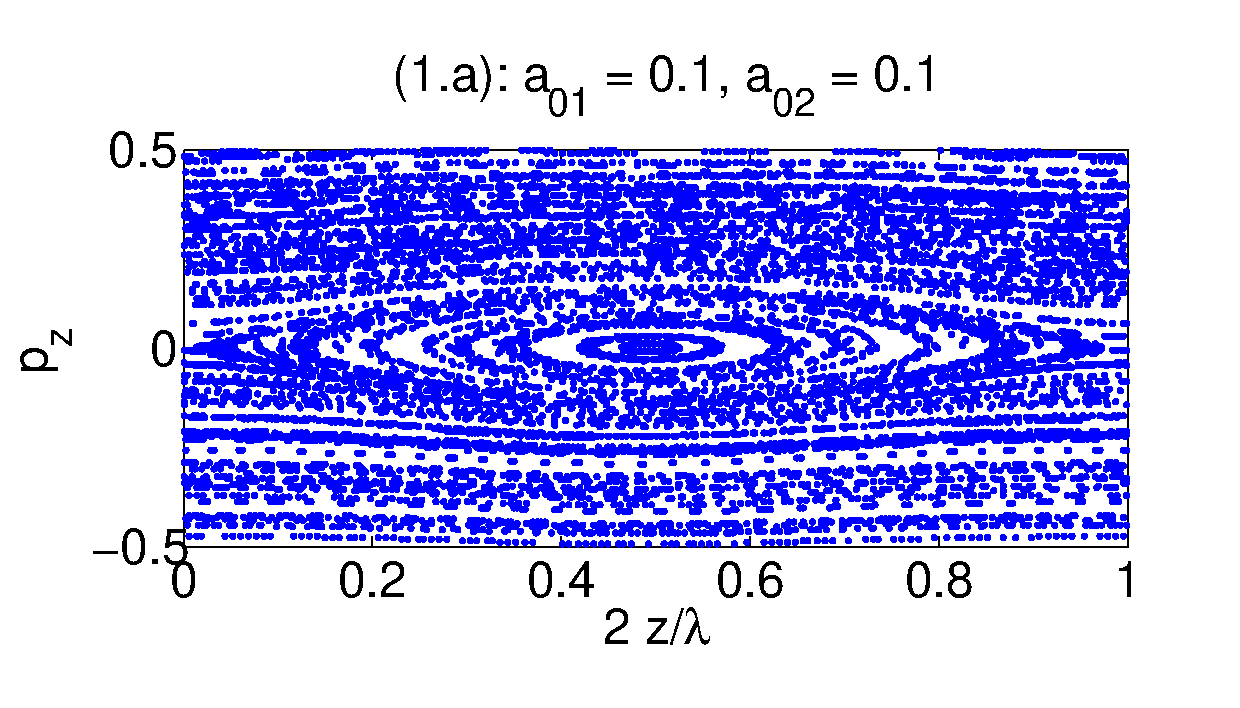
\includegraphics[width =8cm]{../chapitre2/images/StocasticHeating_fig1A.pdf}&
%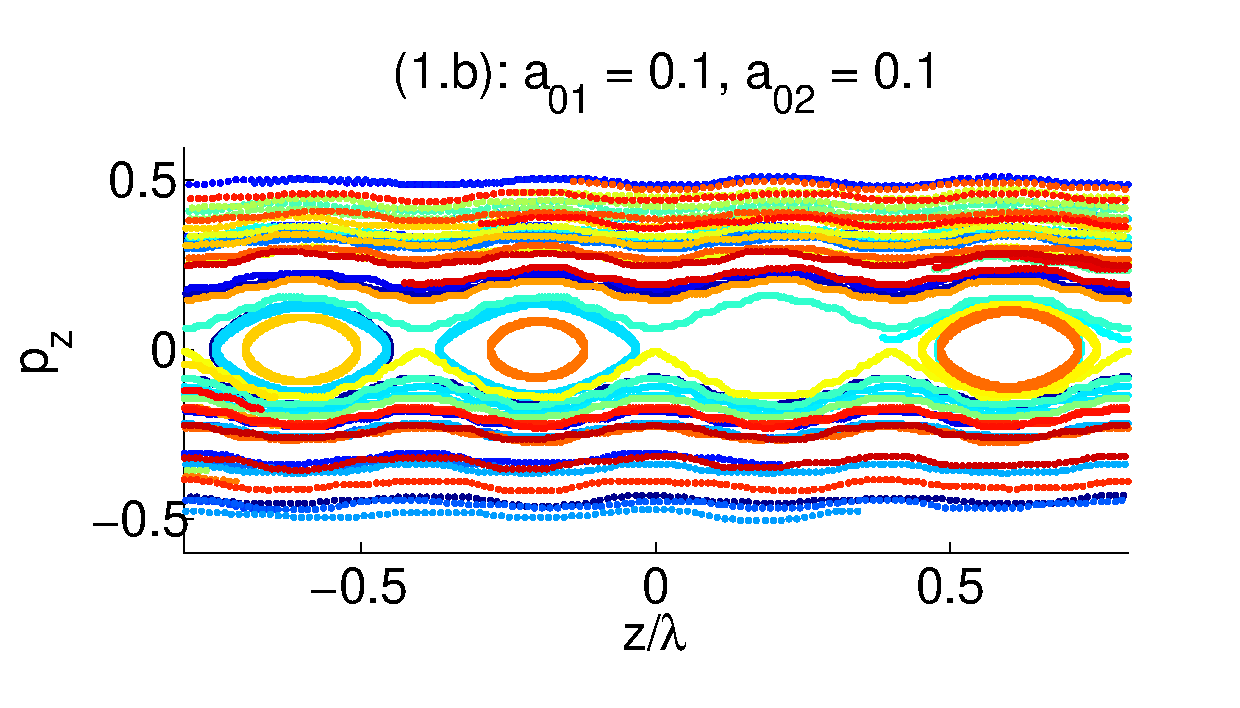
\includegraphics[width =8cm]{../chapitre2/images/StocasticHeating_fig1B.pdf}\\
%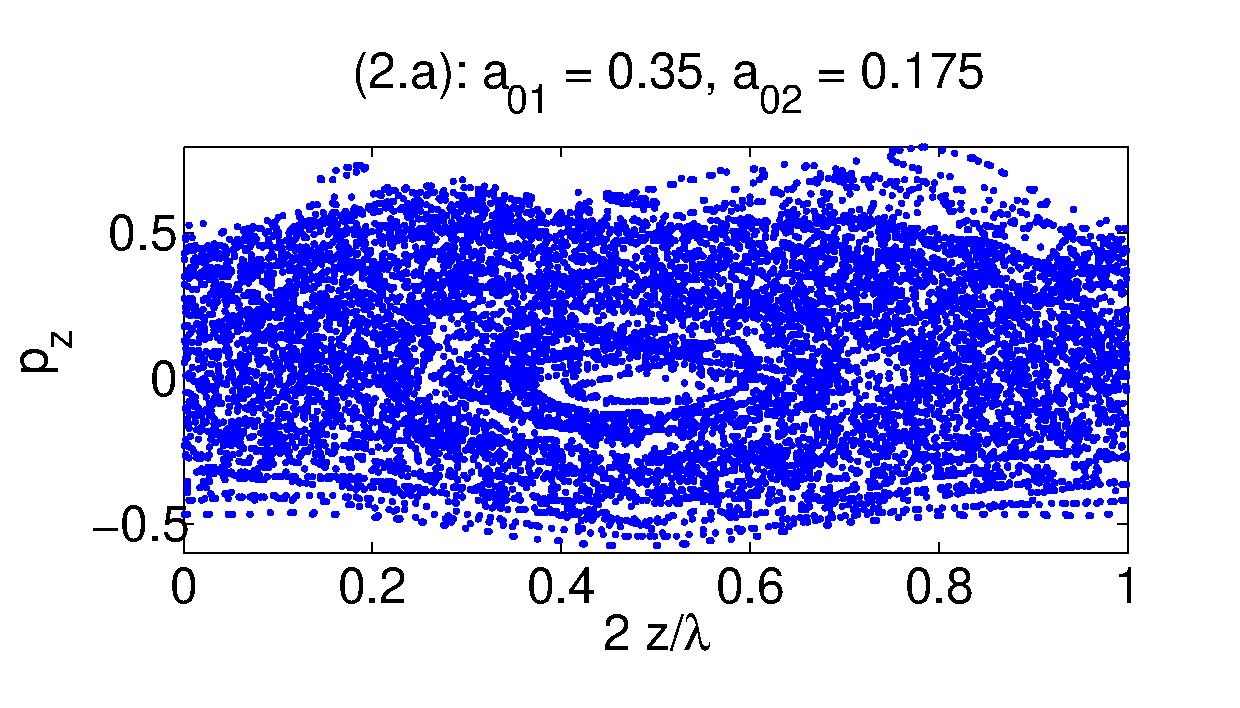
\includegraphics[width =8cm]{../chapitre2/images/StocasticHeating_fig2A.pdf}&
%\includegraphics[width =8cm]{../chapitre2/images/StocasticHeating_fig2B.pdf}\\
%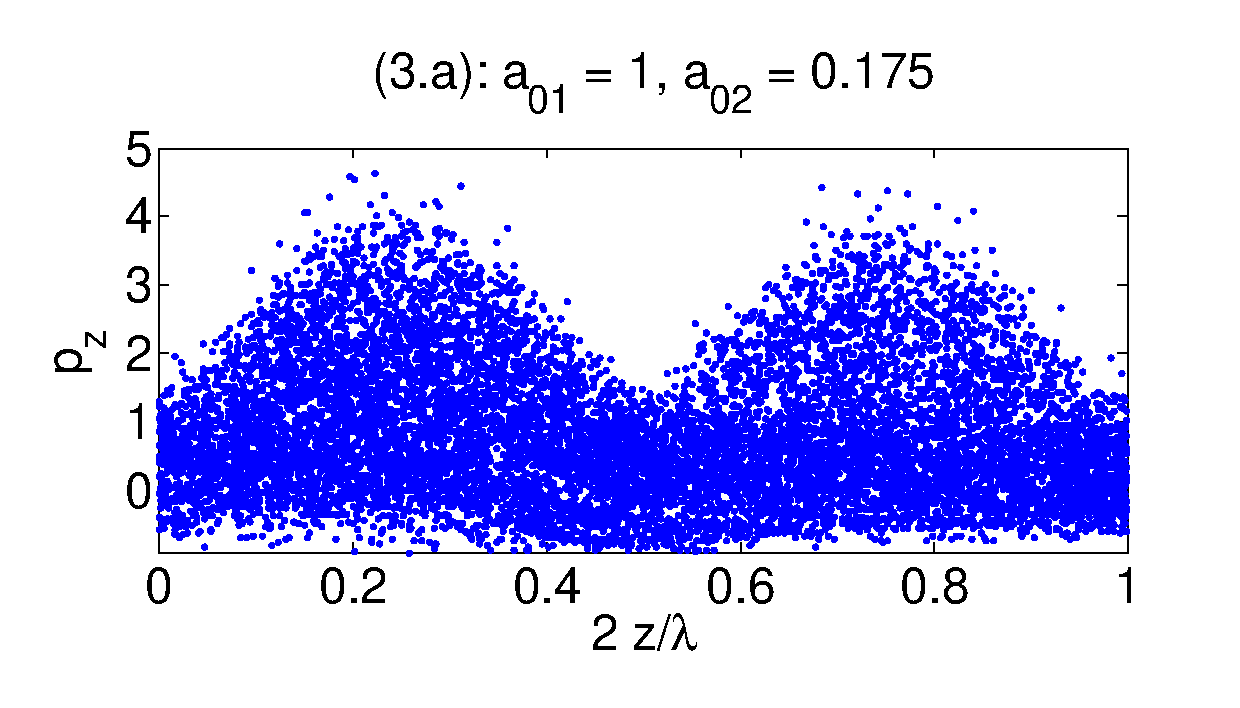
\includegraphics[width =8cm]{../chapitre2/images/StocasticHeating_fig3A.pdf}&
%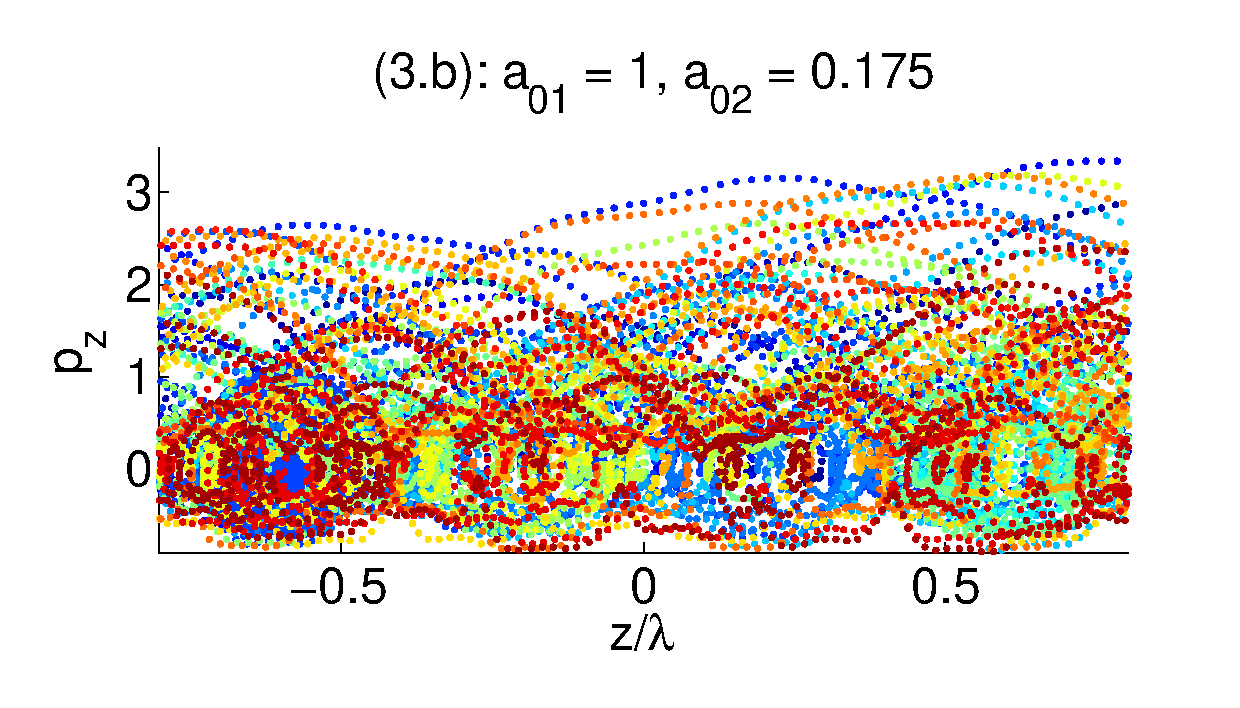
\includegraphics[width =8cm]{../chapitre2/images/StocasticHeating_fig3B.pdf}
%\end{tabular}
%}
%\caption{\label{Fig:StocasticHeating}(a) Poincare sections of electrons. Initially, 121 test electrons are randomly distributed with $(z_0,p_{z0})$ in the volume $[-3.75\lambda \ \ 3.75\lambda]\times[-0.5 \ \ 0.5]$  (b) Correponding phase diagram in the $(z,p_z)$ plane. Each color represents a different electron.}
%\end{figure}
%
%
%We illustrate the choatic behavior by plotting the Poincare section of 121 test electrons with random initial conditions injected in two counterpropagating \g{plane waves} of amplitude $a_{01}$ and $a_{02}$. The intersection plane is defined in the moving frame $(z + ct) = 0[\lambda]$ to account for the periodicity of the laser (the Poincare section is also called "Stroboscopic section" with this definition). In the reference frame, we record the electron phase $z - ct = z + z = 2z$ brought back to the $[0 \ \ \lambda]$ intervalle by modulus division.
% The result is plotted in Fig~\ref{Fig:StocasticHeating}. For (1.a) $a_{01} = a_{02} = 0.1$ we can clearly identify closed orbitals on the Poincare section which means the electron motion is quasi-periodic. On figure (1.b) we give an equivalent representation of the electron trajectories in phase space $(z,p_z)$ were we can visualize periodic trapping orbits for low $p_z$ values. (2) $a_{01} = 0.35$, $a_{02} = 0.175$: we see a randomization of the dots appearing in the Poincare section and simultaneously none laminar trajectories in phase space. Finally, in case (3) $a_{01} = 1$, $a_{01} = 0.175$ : we are in a chaotic regime with a randomized Poincare section and mixed up electrons trajectories in phase space. A detailed description of this chaotic transition can be found in~\ref{TheseRechatin}.\\
%
%
%It is important to note that in the above analysis, as well as in literature, the study of chaotic heating created by an interference pattern implies long laser durations ( hundreds of optical cycles )\cite{sheng2002stochastic}.
%Analytically, \g{continuous plane waves} are useful for an Hamiltonian formulation, which means the pulse extends infinitely in both time and space. 

However, when one drastically reduces the spatial dimensions of the laser focus (strong focusing geometry) and temporal duration (fs laser pulses), the establishment of stochastic heating is no longer possible when (i) the mean propagation length of an electron compares with the laser Rayleigh length and (ii) the establishment of chaos is long relative to the pulse duration. In our solid-target experiment, the interference field is located at the target surface over a distance comparable to the Rayleigh length such that chaotic heating will be negligible. 

\subsection{Conclusion}

This review of different heating mechanisms shows the high sensitivity of electron acceleration to the plasma scale length and electron density of the plasma. Therefore, in order to study each of these mechanisms in experiments, it is necessary to ensure that there is no uncontrolled preionisation of the target prior to the interaction. At the same time, reaching $\sim 1\,\mathrm{MeV}$ electron energies and above requires relativistic intensities. This means that the laser contrast should be $\ge 10^{9-10}$ up to a few picoseconds before the pulse peak to prevent the thermal expansion of the plasma~\cite{kruer1988physics}, which increases the complexity of the laser system because of the need for efficient contrast cleaning. This explains why most experiments have been conducted at high-intensity and long plasma scale lengths~\cite{kodama2000long,chen2001effects,baton2003evidence,Wang2010,chen2006surface} or low intensity ($a_0 < 0.1$) and short plasma scale lengths~\cite{chen2001hot,li2003spatial}. Very few high-intensity experiments ($a_0\sim1$) with gradient control ($L <\lambda$) have been reported~\cite{mordovanakis2009quasimonoenergetic,thevenet2015}. \\


\noindent In the following section, we present our experimental results  on electron acceleration for very short plasma scale length at near-relativistic intensities. We simultaneously detected high-order harmonic emission in the specular direction of the driving laser to increase our comprehension of the plasma mirror dynamics on sub-femtosecond time scales. We will consider further the important role played by (i) the space-charge field created at the surface of the plasma during the interaction and (ii) address the interaction of electrons with the reflecting laser in vacuum in Chapter~\ref{Laser-electron interaction in vacumm}.

\section{Simultaneous HHG and electron detection}\label{section:Simultaneous HHG and electron detection}

\subsection{Description of the experiment}

In our experiment, we simultaneously detect high-order harmonics and the electrons generated on our plasma mirror as a function of the gradient scale length. Our laser pulse is focused on the fused silica rotating target by means of a f/1.2 off axis parabola. The focal spot is $1.7\,\mathrm{\mu m}$ at FWHM and the intensity $\sim 10^{17-18}\,\mathrm{W/cm^2}$($0.2 \le a_0 \le 1$).
A few percents of the main pulse energy is picked off using a beam splitter and focused on target using the same parabola, with an intensity of~$\sim10^{14}\,\mathrm{W/cm^2}$ and a focal spot $5$ times greater, to ensure homogeneous plasma conditions. The laser characteristics on target are detailed in Chapter~\ref{chapter:Overall presentation of the laser system}.\\

\noindent \g{HHG detection:} Already described in~\ref{subsub:Experimental set-up for HHG measurement}. The harmonics of the laser are detected in the specular direction with a concave grating positioned behind a vertical slit.
 The beam is diffracted in the optical plane only and keeps diverging in the other direction. The resulting signal is detected on an MCP.  \\

\noindent \g{Electron detection:} Ballistic electrons are detected using a fluorescent screen called "LANEX" emitting at $546\,\mathrm{nm}$, corresponding to phosphor emission. The detection efficiency is shown in Fig~\ref{fig:LanexResponse}: only electron of energy$>150\,\mathrm{keV}$ are detected. The $6\times 17\,\mathrm{cm}$ LANEX screen is positioned $10\,\mathrm{cm}$ parallel to the target without blocking the HHG entrance slit. The angular electron emission profile in this geometry is recorded as a function of $\theta \in [-20^{\circ}\ ; \ 35^{\circ}]$, the angle to normal in the azimuthal plane of incidence and $\phi\in [-20^{\circ} \ ; \ 20^{\circ}]$, the angle being defined in the tangential plane.


\begin{figure}[H]
\centering
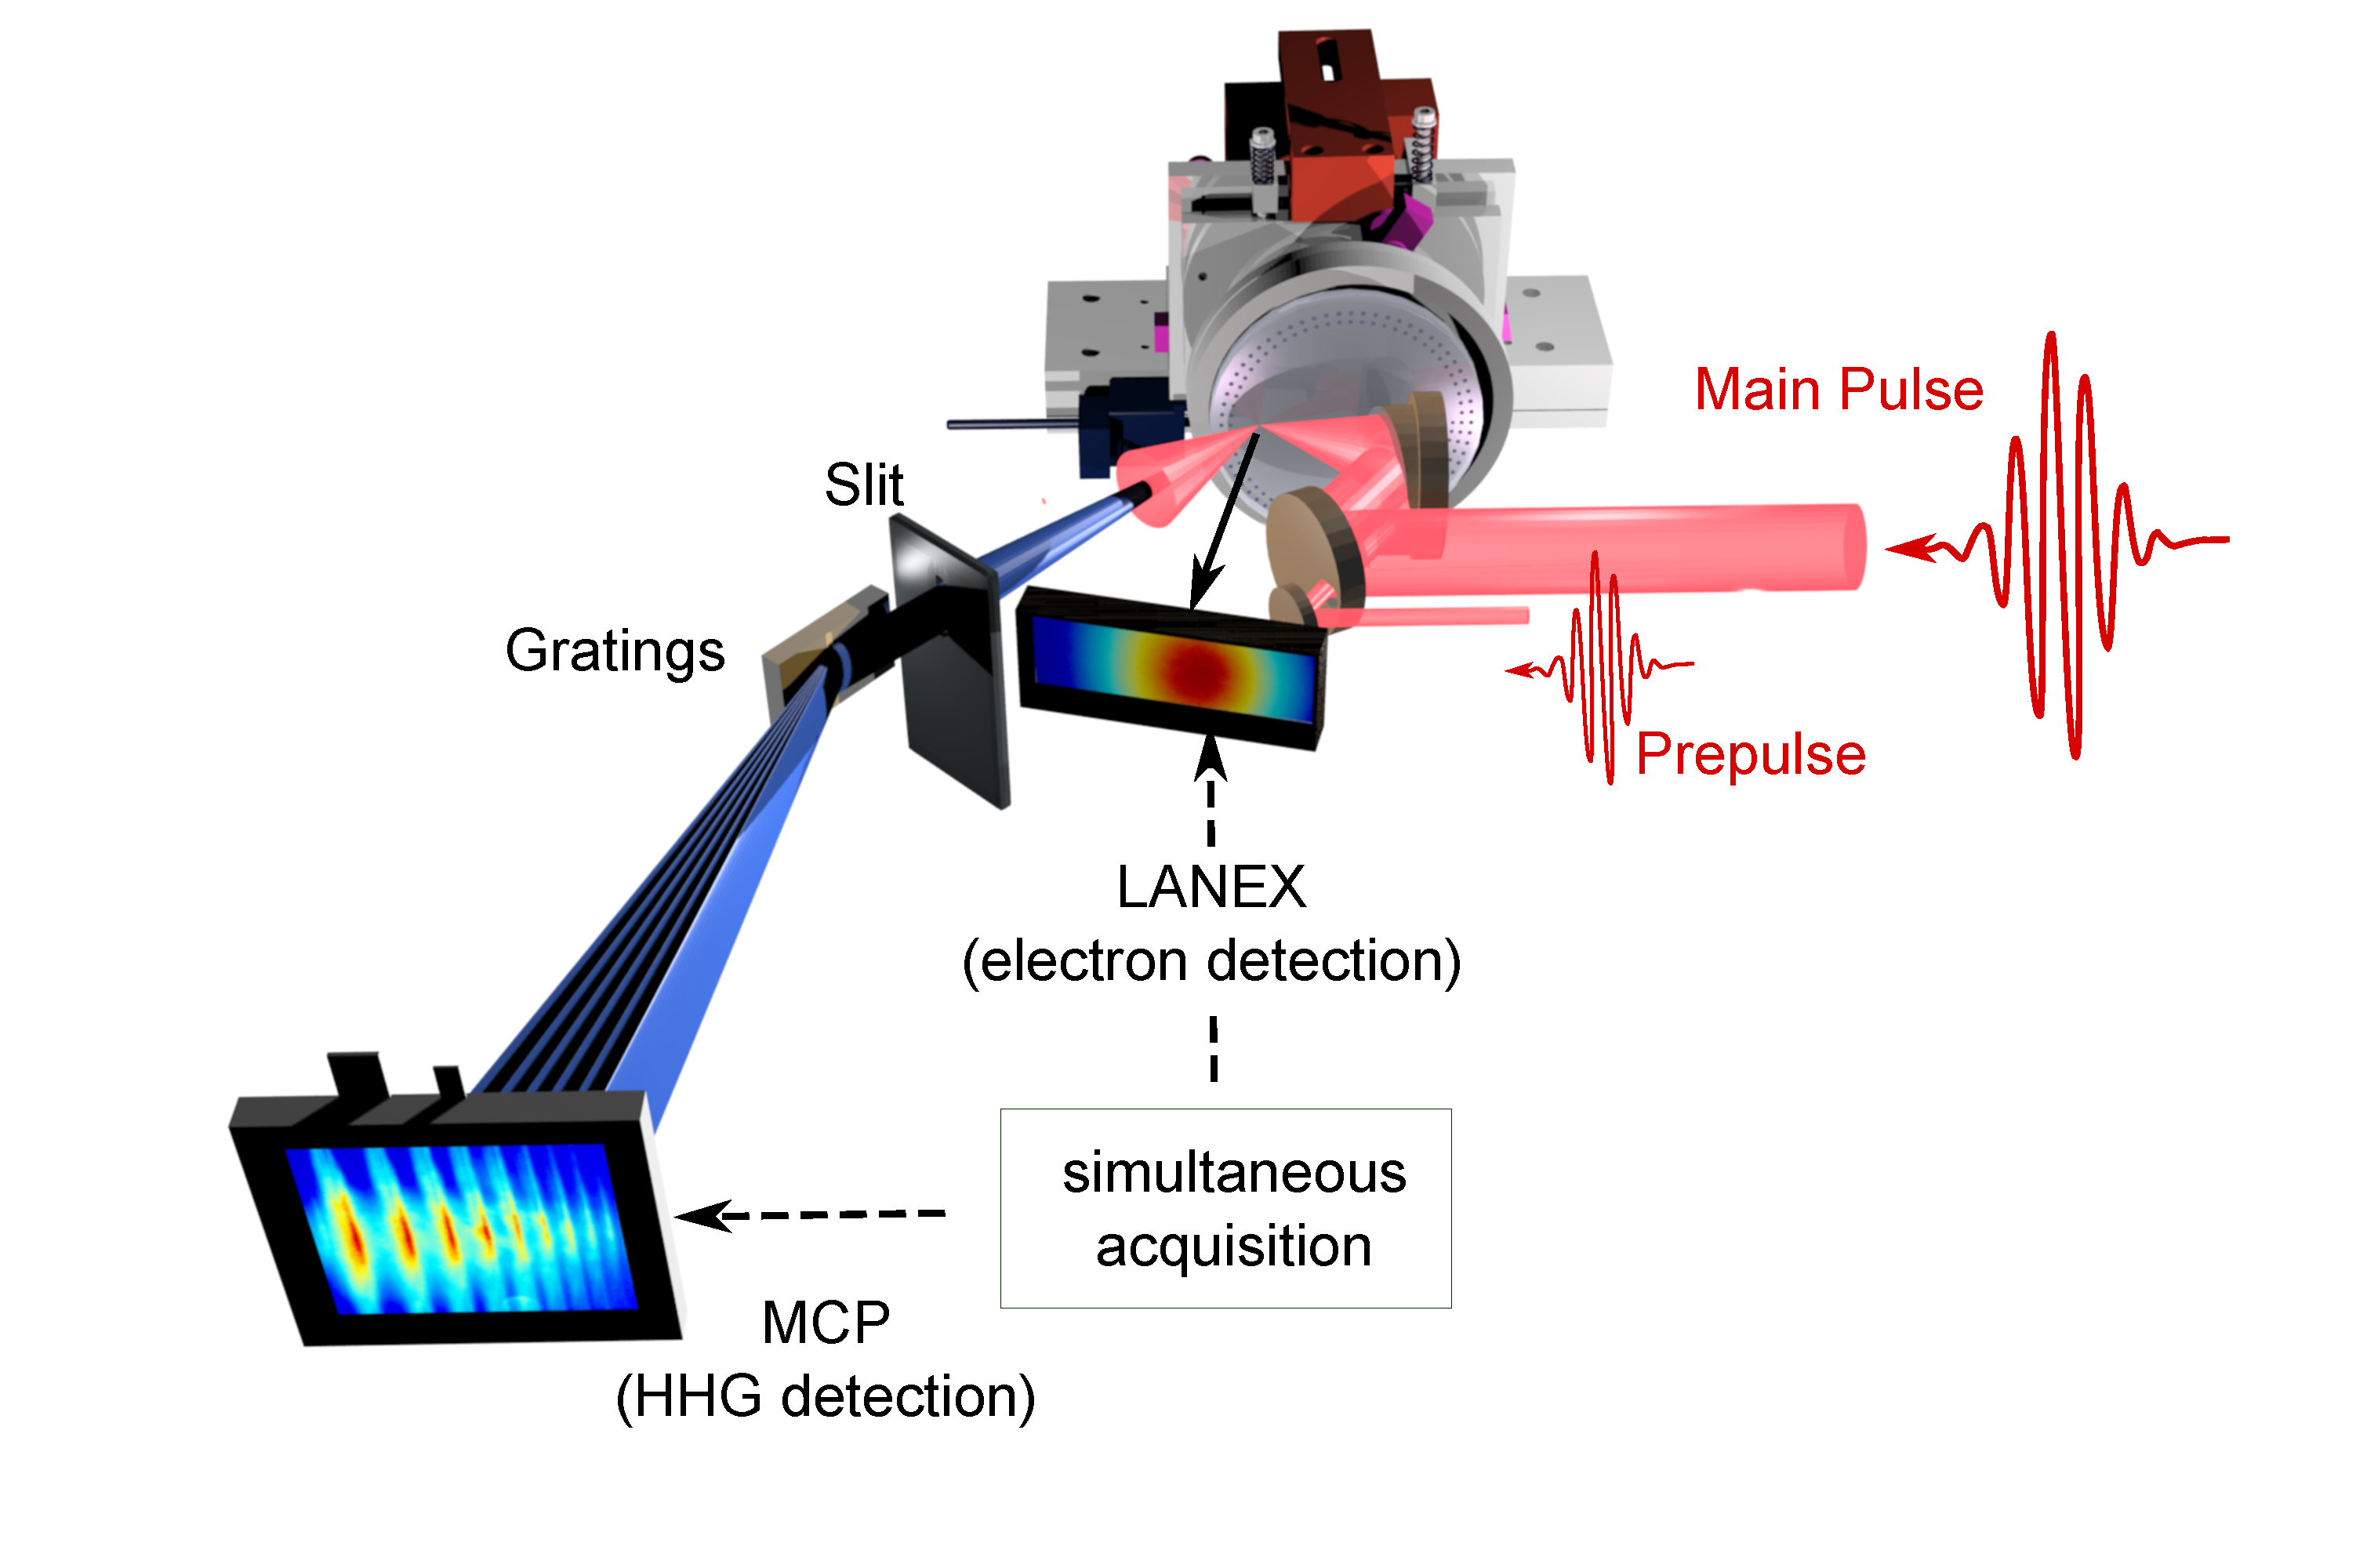
\includegraphics[width =\textwidth]{../chapitre4/images/SETUP.pdf}\\
\caption{\label{fig:SETUP} Experimental setup: Main pulse and prepulse are focused on a rotating fused silica target with an off-axis parabola. The HHG signal is detected in the specular direction and the electronic emission with a LANEX screen placed normal to the target. Both signals are recorded simultaneously for each firing sequence (integration over $\sim 100$ laser shots). Prepulse intensity on target:$\sim 10^{14}\,\mathrm{W/cm^2}$, Main laser intensity on target $\sim 10^{18}\,\mathrm{W/cm^2}$.}
\end{figure}

\begin{figure}[H]
\centering
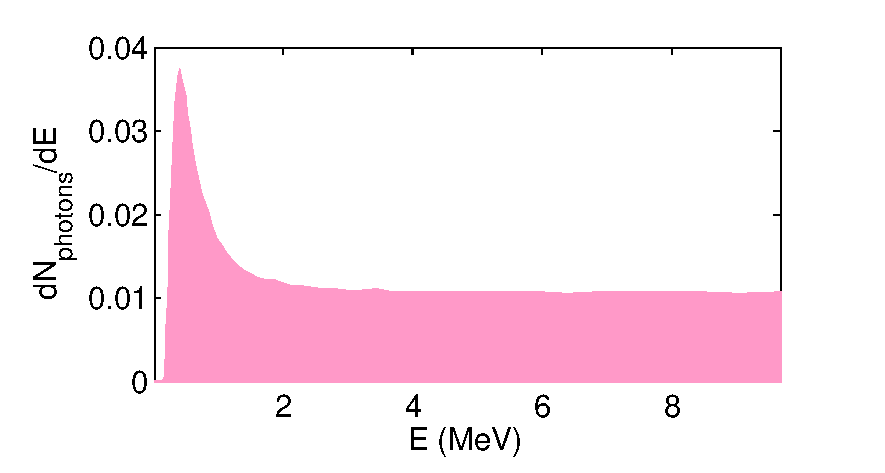
\includegraphics[width =0.6\textwidth]{../chapitre4/images/LanexResponse.pdf}\\
%\captionsetup{justification=centering}
\caption{\label{fig:LanexResponse}LANEX response based on Monte Carlo simulations \cite{glinec2006absolute}}
\end{figure}



\subsection{CWE/electron anticorrelation vs plasma scale length}\label{subsub:CWE/electron anticorreleation with plasma scale length}

By varying the plasma scale length from arbitrarily small values $L\sim \lambda/100$ to $L\sim \lambda$ using the pump-probe delay, we observe that the emission of harmonics
and electrons is anticorrelated: CWE emission is efficient at short plasma scale length $L< 0.05 \lambda$, while electron ejection from the target is optimal for longer gradients $L\sim 0.1\lambda$.

\begin{figure}[H]
\centering
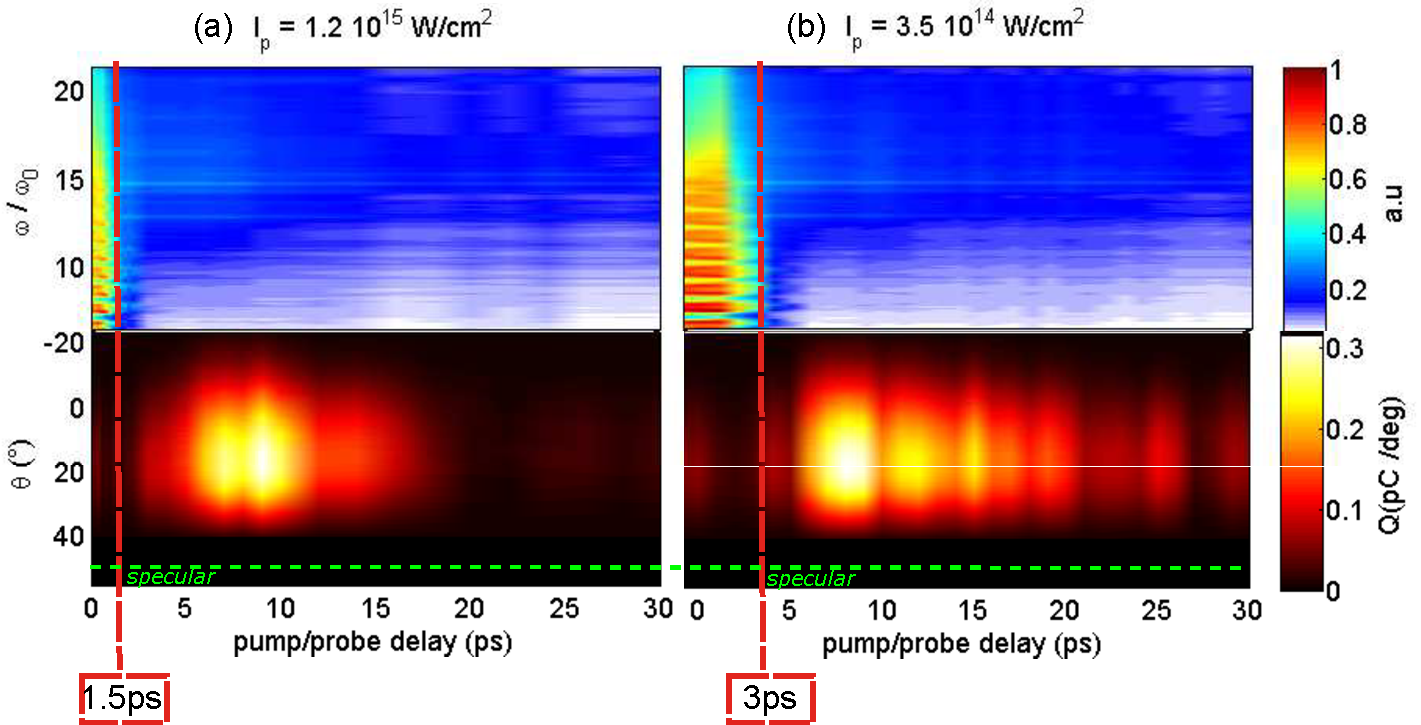
\includegraphics[width =\textwidth]{../chapitre4/images/resultsFinalExp.pdf}\\
\caption{\label{fig:resultsFinalExp} Experimental results comparing simultaneous harmonic and electron emission for a prepulse (pump) intensity of (a)$I_p = 1.2 \times 10^{15}\,\mathrm{W/cm^2}$ and (b)$I_p = 3.5\times 10^{14}\,\mathrm{W/cm^2}$. In both cases, the main (probe) laser intensity is $a_0 = 0.85$. The LANEX detection range in the horizontal plane is $\theta \in [-20^{\circ} \ \ 35^{\circ}]$. The azimuthal spread was artificially extended to show the specular angle of $49.3^{\circ}$ indicated by the green dotted line}
\end{figure}

\noindent Experimental results are gathered in Fig~\ref{fig:resultsFinalExp}. The harmonic spectra are integrated along the divergence angle and the LANEX signal along its tangential coordinate $\phi$. As a result, we present the evolution of the harmonic intensity and the angular electron distribution as a function of the pump-probe delay, for two different prepulse intensities namely (a)$I_p = 1.2 \times 10^{15}\,\mathrm{W/cm^2}$ and (b)$I_p = 3.5\times 10^{14}\,\mathrm{W/cm^2}$. In both cases, the anticorrelation pattern is the same: as we increase the pump-probe delay, the harmonic signal drops and we observe a rise of the electron emission signal on the LANEX. The sharp drop in harmonic generation is marked on Fig~\ref{fig:resultsFinalExp} by a vertical red dotted line. Harmonics disappear for (a)$t \approx 1.5\,\mathrm{ps}$ or (b)$t \approx 3\,\mathrm{ps}$ depending on the prepulse intensity, for the same main pulse intensity $a_0 = 0.85$. This is consistent with an increased expansion velocity of the plasma $\propto \sqrt{I_p}$, which predicts that the plasma expands $\sim 1.8$ times faster in (a) than in (b).The optimal delay for electron generation is not very well defined in~\ref{fig:resultsFinalExp}, but rather spans over several gradient lengths. The optimal value in $(b)$ is reached for $t\approx 8\,\mathrm{ps}$, which corresponds to $L\sim 0.1\lambda$. However, for long pump-probe delays, the electron emission drops after a delay again consistent from (a) to (b), if we account for a variation of the expansion velocity $\propto \sqrt{I_p}$.\\% In other words, we have shown in this experiement that changing the prepulse intensity

\g{Why this anticorrelation?}\\

\noindent We already answered half of this question in Section~\ref{section:Harmonic plasma response to Brunel electrons} when we explained that CWE mechanism is only efficient at short gradient scale length. For electrons to escape the plasma into vacuum, they need to gain sufficient energy is in the space-charge field created at the surface to escape Brunel's confined orbitals~\cite{Geindre2010,bocoum2016anticorrelated}, which is why $L$ needs to be increased. 

\begin{figure}[H]
\begin{center}
\makebox[\textwidth][c]{
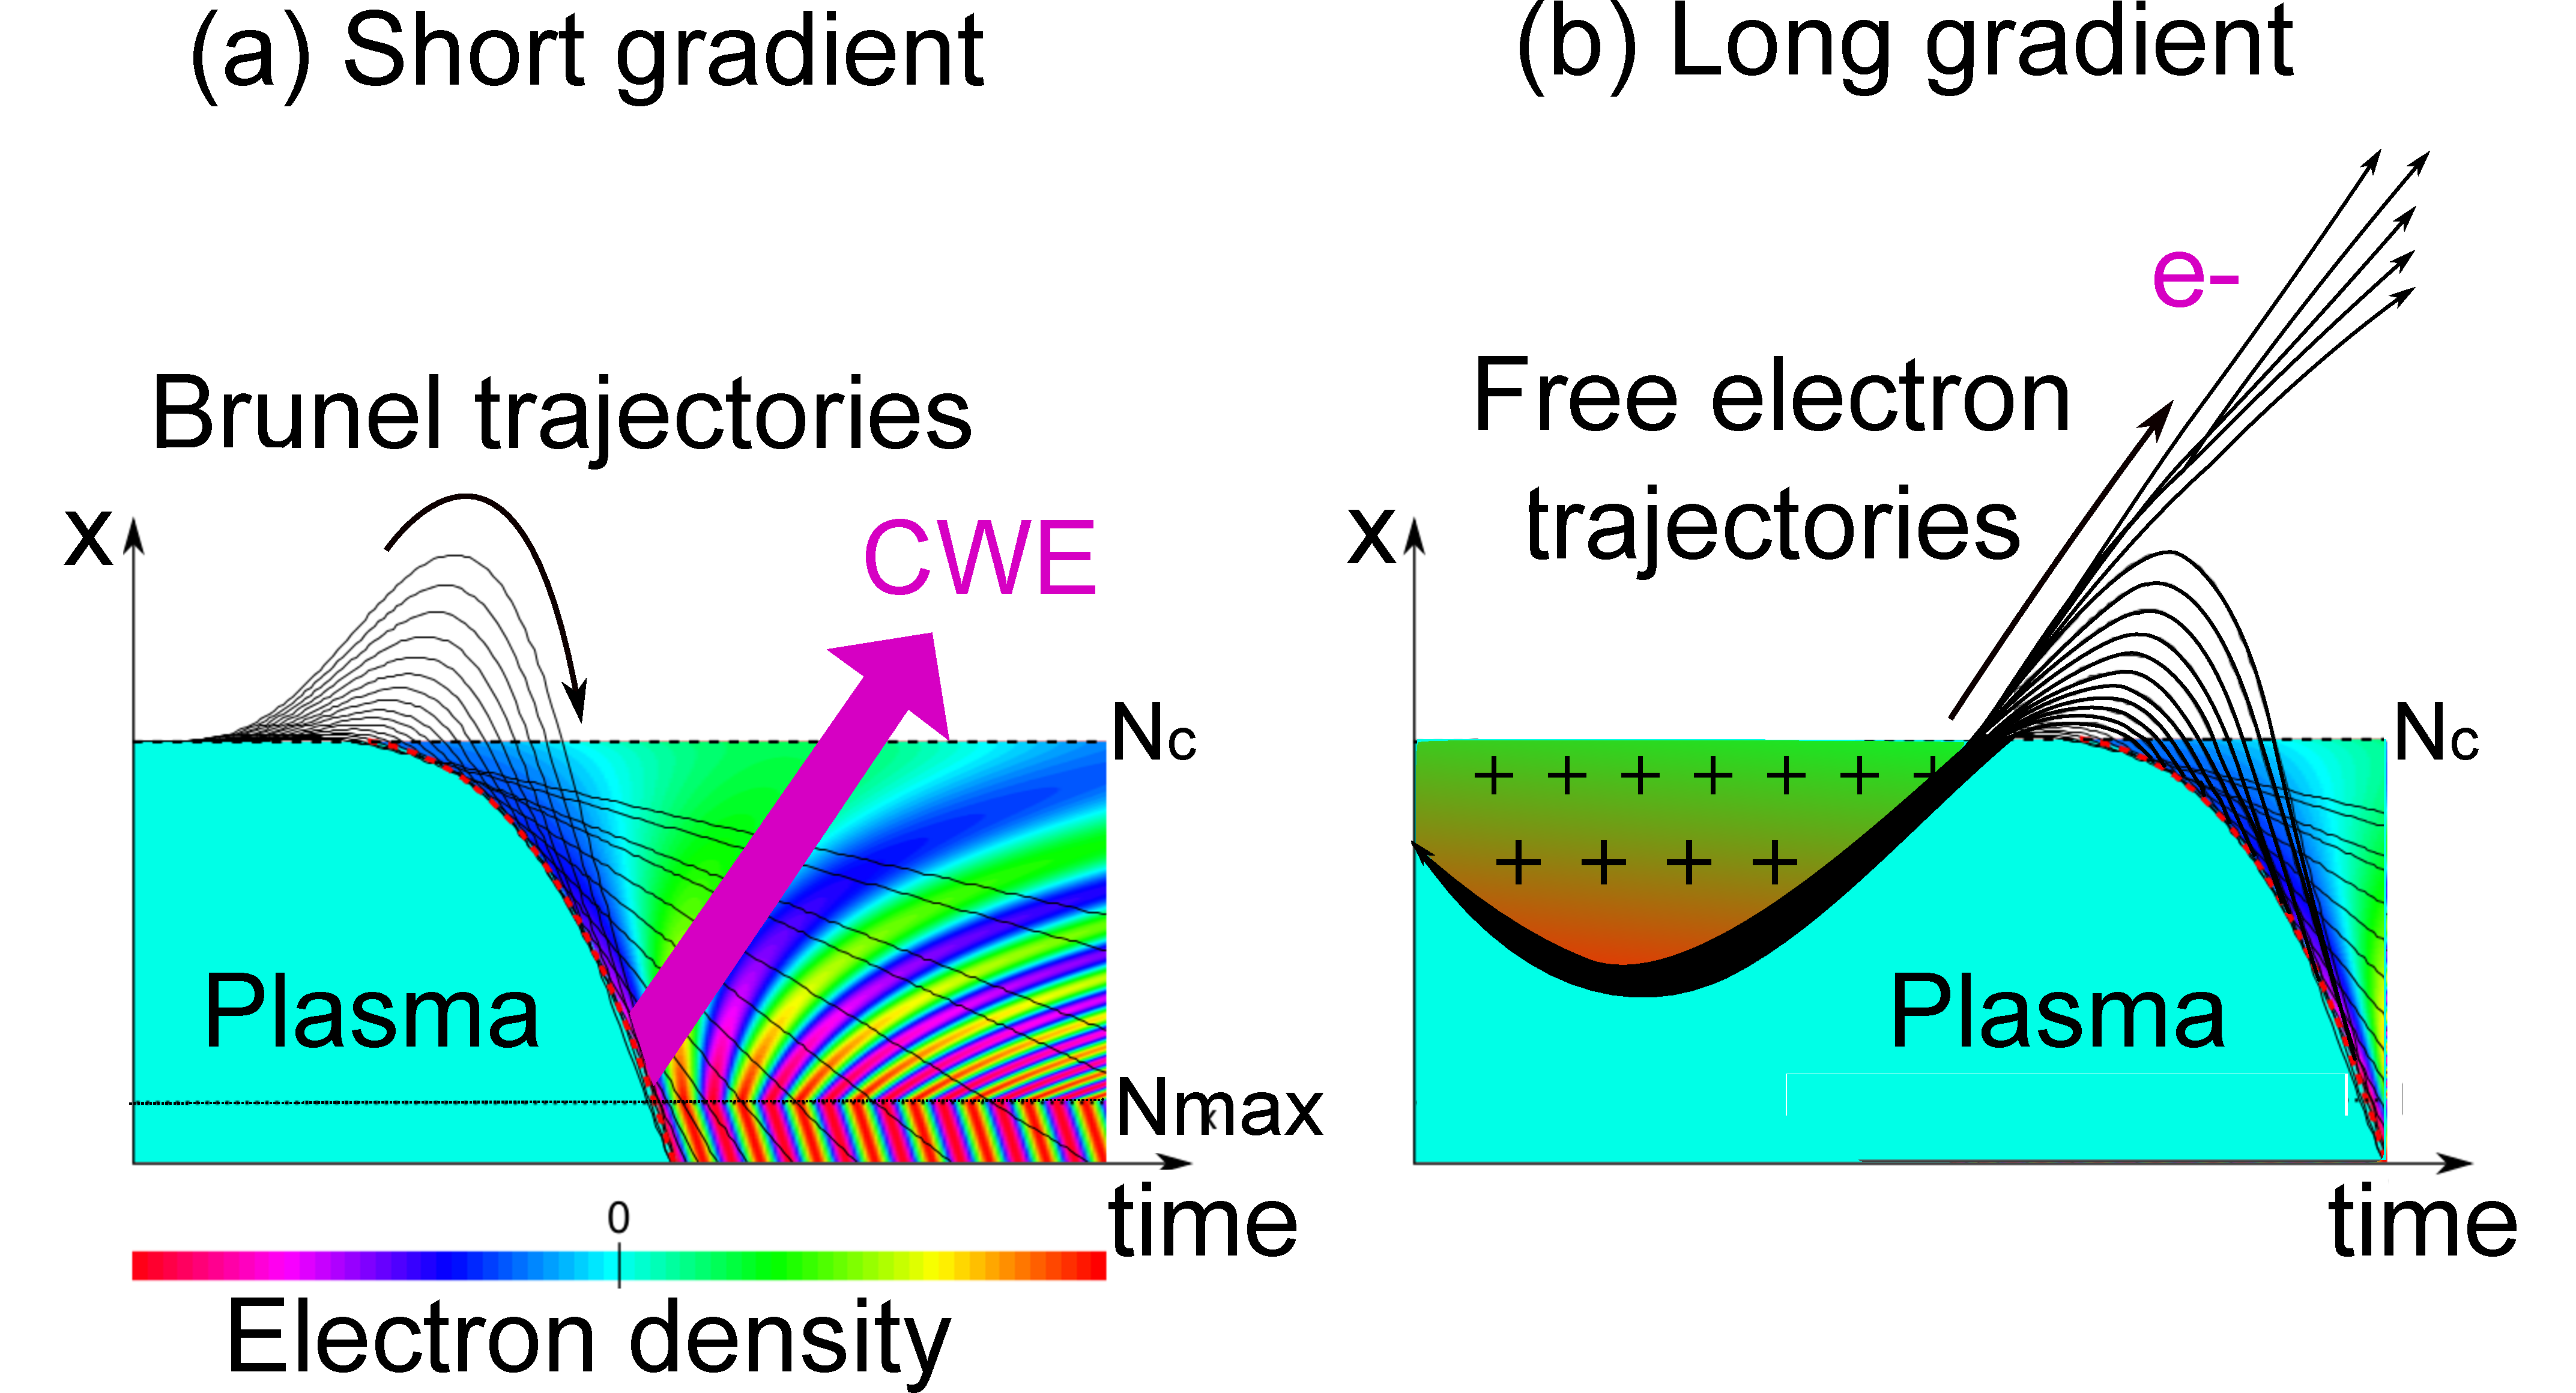
\includegraphics[width = 0.6\textwidth]{../chapitre4/images/figure1.pdf}}
\end{center}
\caption{\label{fig:figure1}Artistic representation of HHG/electron anticorrelated behavior of plasma mirrors. (a) Efficient CWE generation for $L/\lambda < 0.05$ (b) Efficient electron ejection for $L/\lambda\sim 0.1$}
\end{figure}

\noindent As we already described in Section~\ref{section:Brunel absorption mechanism}, the plasma field $E_P(x)$ due to charge separation at the surface is simply evaluated using an exponential profile:

\begin{equation}
E_P(x) = \frac{1}{\epsilon_0}\int_{x}^{\infty}en_ce^{-(x'-x_c)/L}dx' = \frac{m_e}{e} \omega_0^2 L\exp(-\frac{x-x_c}{L})
\label{eq:PlasmaContribution}
\end{equation}

\noindent where $x_c$ denotes the critical surface coordinate with density $n_c$, and $L$ the gradient scale length. If in addition we impose that the plasma field completely screens the laser when all electrons are pushed below $x<x_s$, then we have:

\begin{equation}
\label{eq:a0vsplasma}
a_0  c= \omega_0L\exp(-\frac{x_s-x_c}{L})
\end{equation}

\noindent We calculate, for this fixed value of $x_s$ the work provided by the plasma using Eq~\ref{eq:PlasmaContribution}:

$$
W(E_P) = \int_{x_s}^{\infty}-eE_P(x)dx = m_e \omega_0^2  L^2 \exp(-\frac{x_s-x_c}{L})
$$
$$
= 2\pi  (m_e c^2)   a_0  \frac{L}{\lambda_0} 
$$

\noindent This gives us a scaling for the electron final energy when the plasma contribution only is considered:
\begin{equation}
W(E_P)(\,\mathrm{keV}) = 3.2 \times 10^3 a_0  \frac{L}{\lambda_0} 
\label{eq:ScaleLength}
\end{equation}

\noindent This simple scaling will of course only be accurate for very short plasma scale length. For $L>\lambda$, the laser propagates in the underdense region and the hypotheses made to derive the scaling are no longer valid.
For $L/\lambda < 1$ and $a_0\sim 0.8$ we have $W(E_P) < 500 \,\mathrm{keV}$, which is consistent with the experimental data later presented in~\ref{subsub:Spectral measurement}.

\noindent Finally, comparing the two scaling laws obtained respectively for the laser and the plasma, we can write that the plasma becomes "more efficient" in accelerating the electrons when:
$$
 L/\lambda > a_0/6.4
$$

\noindent In Fig~\ref{fig:20140808FocusScanElectronVShhgs}, we show how the anticorrelated behavior can be used to track the position of the focus at high-energy. Indeed, thermal effects in the laser chain can lead to few-micron defocusing of the laser on target, even when only reflective optics are used. A high-intensity diagnostic of the focus position therefore becomes very useful.
\noindent Removing the prepulse, we degraded the laser contrast by misaligning the Glan polarizer after the XPW(cf Chapter \ref{chapter:Overall presentation of the laser system}), which leads to consequent preionisation of the target. We observe the signal obtained for both HHG and electrons when scanning the focal spot. Indeed, if we compare two scans at low ($a_0 = 0.25$) and high ($a_0=0.4$) intensity, we find that again, in both cases HHG and electron emission are anticorrelated but in the high-energy case, the electron emission decreases at focus because the contrast is so poor. Defocusing the laser in both directions allows to recover the signal. Note that this scan constitutes a good test to probe the quality of the laser contrast at full energy.



\begin{figure}[H]
\begin{center}
\makebox[\textwidth][c]{
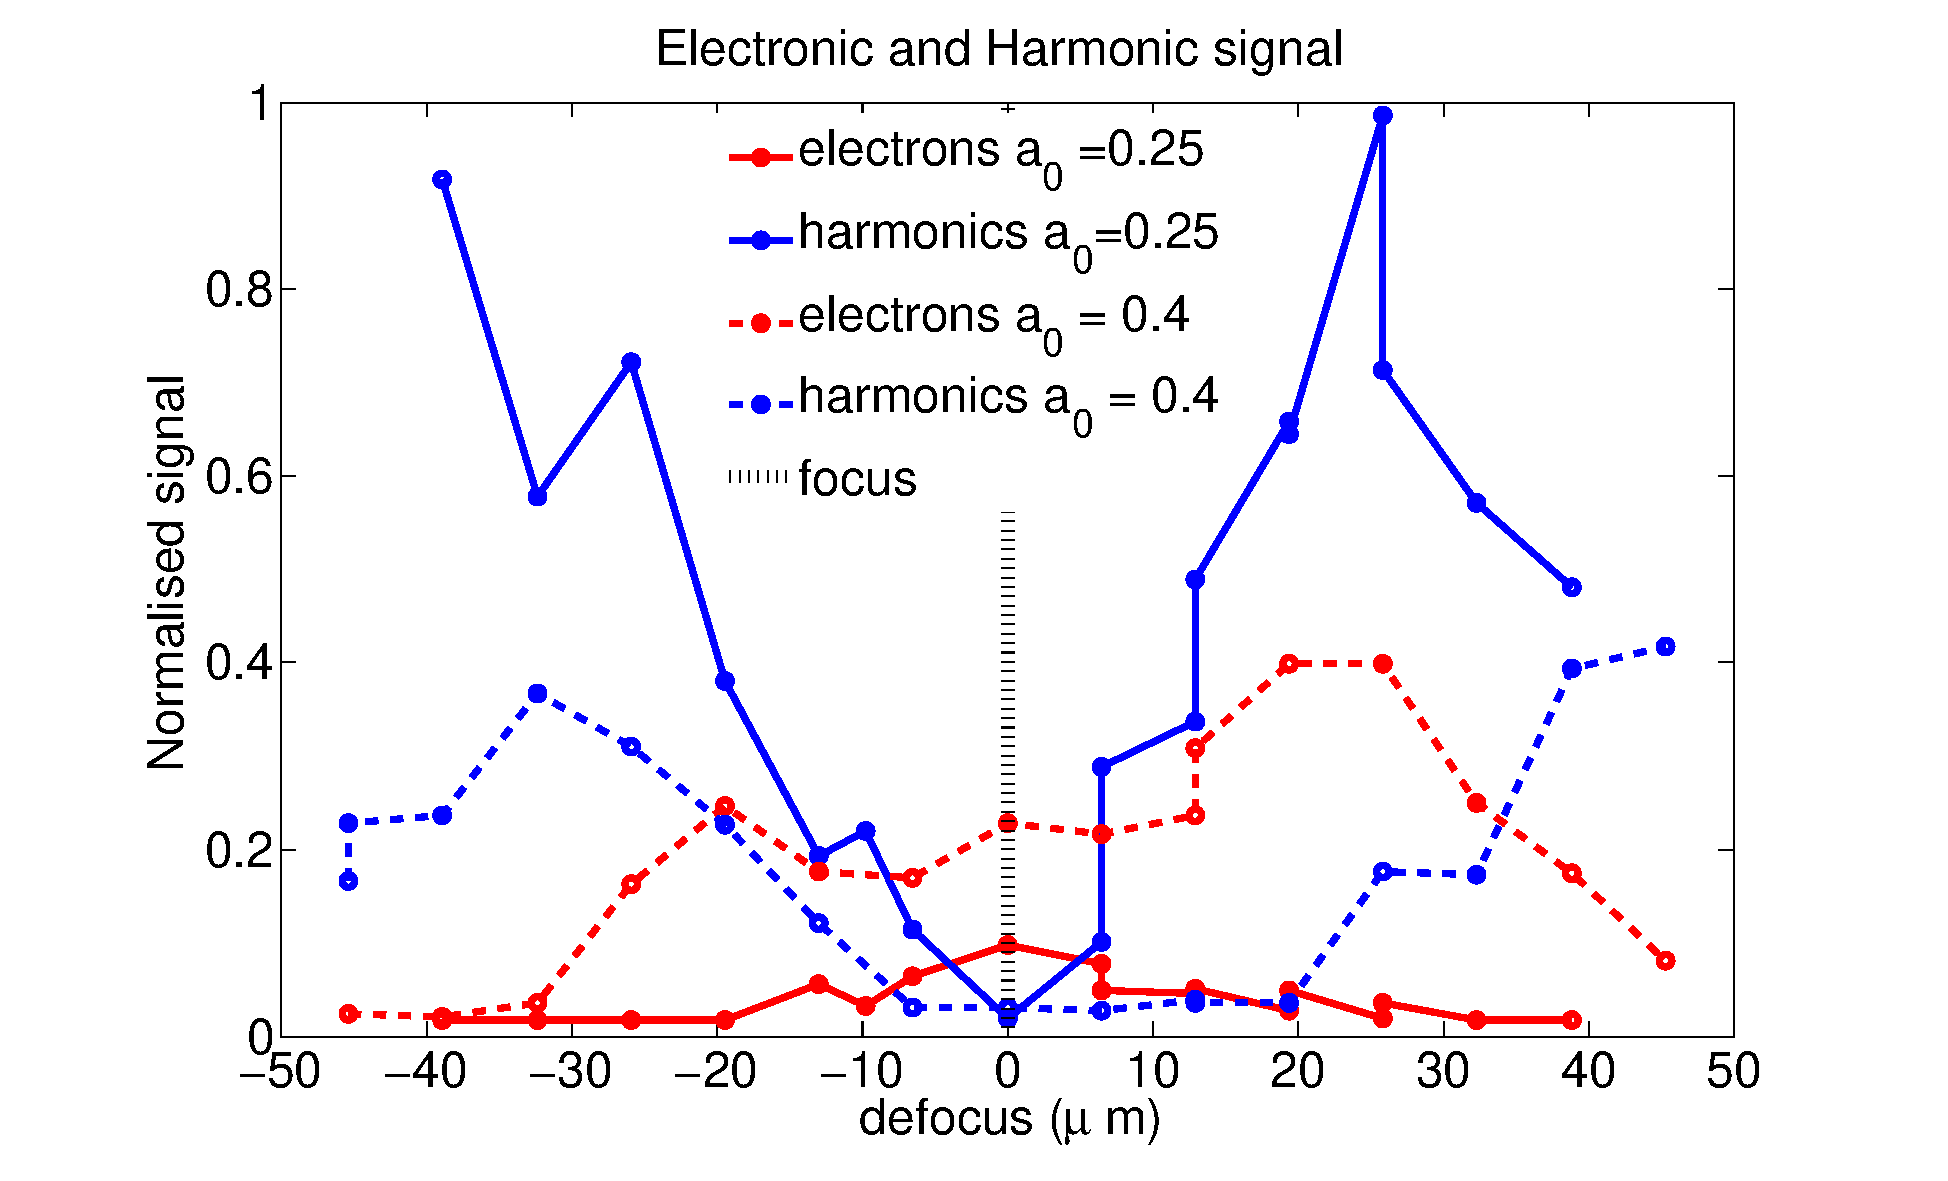
\includegraphics[width = \textwidth]{../chapitre4/images/20140808FocusScanElectronVShhg.pdf}}
\end{center}
\caption{\label{fig:20140808FocusScanElectronVShhgs} Integrated counts on MCP and LANEX measuring respectively the harmonic and electron generation efficiencies with respect to focus position in $\mu m$. The focal spot size is $3.5\,\mathrm{\mu m}$ FWHM.}
\end{figure}




\subsection{PIC simulations}

We performed 2D simulations using  the particle-in-cell simulation code EPOCH~\cite{arber2015contemporary} in order to demonstrate the anticorrelated behavior of electron ejection and harmonic generation. We first performed simulations close to our experimental conditions and listed the inputs in table~\ref{tab:inputcode} for the \g{Scan-a0-0.8} simulation run.\\


\begin{center}
\captionof{table}{\label{tab:inputcode}EPOCH input}
\begin{tabular}{|c|c|c|c|c|c|c|c|}
%\caption{\label{tab:inputcode} EPOCH input}
\hline
name &$\theta_i$ & $\lambda$ & $a_0$ & $\tau_{fwhm}$ & $n/n_c$ & $L_g$ & $w_0$\\
\hline
\g{Scan-a0-0.8}&$45^{\circ}$ & $0.8\,\mathrm{\mu m}$& $0.8$ & $30\,\mathrm{fs}$ & $250$ & $\lambda/80\rightarrow \lambda/2.5$ & $1.8\lambda$\\
\hline
\g{Scan-a0-0.4}&$45^{\circ}$ & $0.8\,\mathrm{\mu m}$& $0.4$ & $30\,\mathrm{fs}$ & $250$ & $\lambda/80\rightarrow \lambda/2.5$ & $3.6\lambda$\\
\hline
\end{tabular}
\end{center}



\begin{figure}[H]
\centering
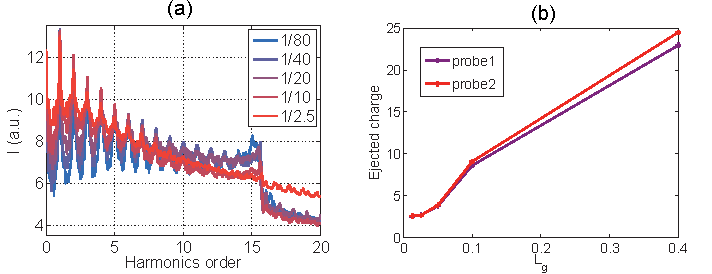
\includegraphics[width =\textwidth]{../chapitre4/images/ROM_corr.pdf}\\
\caption{\label{fig:ROM_corr} \g{Scan-a0-0.8} simulations.(a) HHG emission spectrum in log scale for initial plasma scale length $L_g/\lambda \in [1/80 \ \ 1/2.5]$ (b) Ejected charge in $\,\mathrm{pC/\mu m}$ for respectively $8\lambda$ (probe 2) and $9\lambda$(probe1) from plasma edge ($n_c/5$)}
\end{figure}

\noindent The harmonic emission spectra for different gradient scale lengths is represented in Fig~\ref{fig:ROM_corr}. The clear cut-off at $\omega/\omega_0 = \sqrt{250}\approx 15$ is the signature of CWE emission~\cite{TheseArnaud,TheseHenri}. For $L = \lambda/2.5$, this cut-off disappears as a signature of ROM emission~\cite{TheseArnaud,thaury2010high}. Simultaneously, the ejected charge is detected with two probes placed at respectively $8\lambda$ and $9\lambda$ from the plasma edge (defined at $n_c/5$) and plotted in Fig~\ref{fig:ROM_corr}(b). We observe that long plasma scale lengths favour electron ejection. This simulation confirms the anticorrelation behavior between HHG generation and electron acceleration observed in our experiment. However, to make sure that this conclusion still holds true when harmonics are generated in a purely CWE regime, we performed a second run of simulations \g{Scan-a0-0.4} decreasing the laser intensity to $a_0 = 0.4$. 
\begin{figure}[H]
\centering
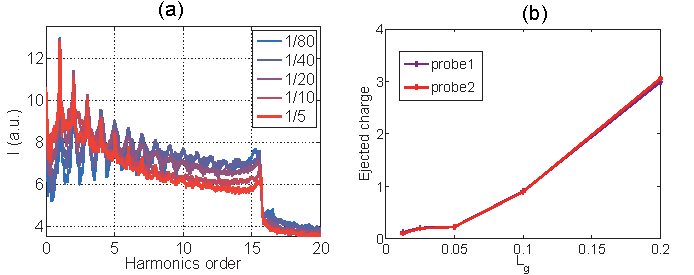
\includegraphics[width =\textwidth]{../chapitre4/images/CWE_corr.pdf}\\
%\captionsetup{justification=centering}
\caption{\label{fig:CWE_corr} \g{Scan-a0-0.4} simulations. (a) HHG emission spectrum in log scale for intial plasma scale length $L_g/\lambda \in [1/80 \ \ 1/5]$ (b) Ejected charge in $\,\mathrm{pC/\mu m}$ for respectively $8\lambda$ (probe 1) and $9\lambda$(probe2) from plasma edge ($n_c/5$)}
\end{figure}


The results are given in Fig~\ref{fig:CWE_corr}. The CWE cut-off is visible for all gradient scale lengths, which confirms that we are in a purely CWE-emission regime, similar to the experiment. The two simulation runs are compared in Fig~\ref{fig:AntiCorrelationSimu} in order to highlight the anticorrelated CWE/electron emission seen in Fig~\ref{fig:20140808FocusScanElectronVShhgs}.\\


\noindent To observe an "optimal" gradient length for electron ejection, we would need to make simulations for much larger $L_g$ values than what is presented in Fig~\ref{fig:AntiCorrelationSimu}(a). The total number of macro-particles in the simulation increases dramatically with $L_g$(565 million for $L_g  = 0.1\lambda$ and 928 million for $ L_g=0.2\lambda$), essentially because modeling HHG requires a very small spatial mesh. For this reason, we only performed two extra simulations for  $L_g = 0.6\lambda$ and $L_g = \lambda$, as shown in Fig~\ref{fig:OptimumObservation_simu}. One can clearly see that the ejected charge finally decreases for very long gradients. This optimum can be located anywhere between $0.2\lambda$ to $\lambda$, but a detailed investigation of its location is extremely time consuming and would anyway be more accurate with 3D simulations to account for the $1/r^2$ decrease of the space charge field from the plasma surface. \\


\noindent Electrons are mostly ejected between $0^{\circ}$ (target normal) and $45^{\circ}$(specular). In the experimental data presented in Fig~\ref{fig:20140808FocusScanElectronVShhgs}, the average angle of emission for the optimal gradient scale length is $\sim 16^{\circ}$, whereas its value is closer to $30^{\circ}$ in our simulations. This apparent discrepancy is actually due to a loss of signal when positioning the LANEX normal to the target. We see in the following that not only, when the LANEX is placed orthogonal to the specular direction, the measurement matches the simulation, but we also observe a hole in the electron angular emission profile typical of ponderomotive interaction of the electron with the reflected laser. 



\begin{figure}[H]
\makebox[\textwidth][c]{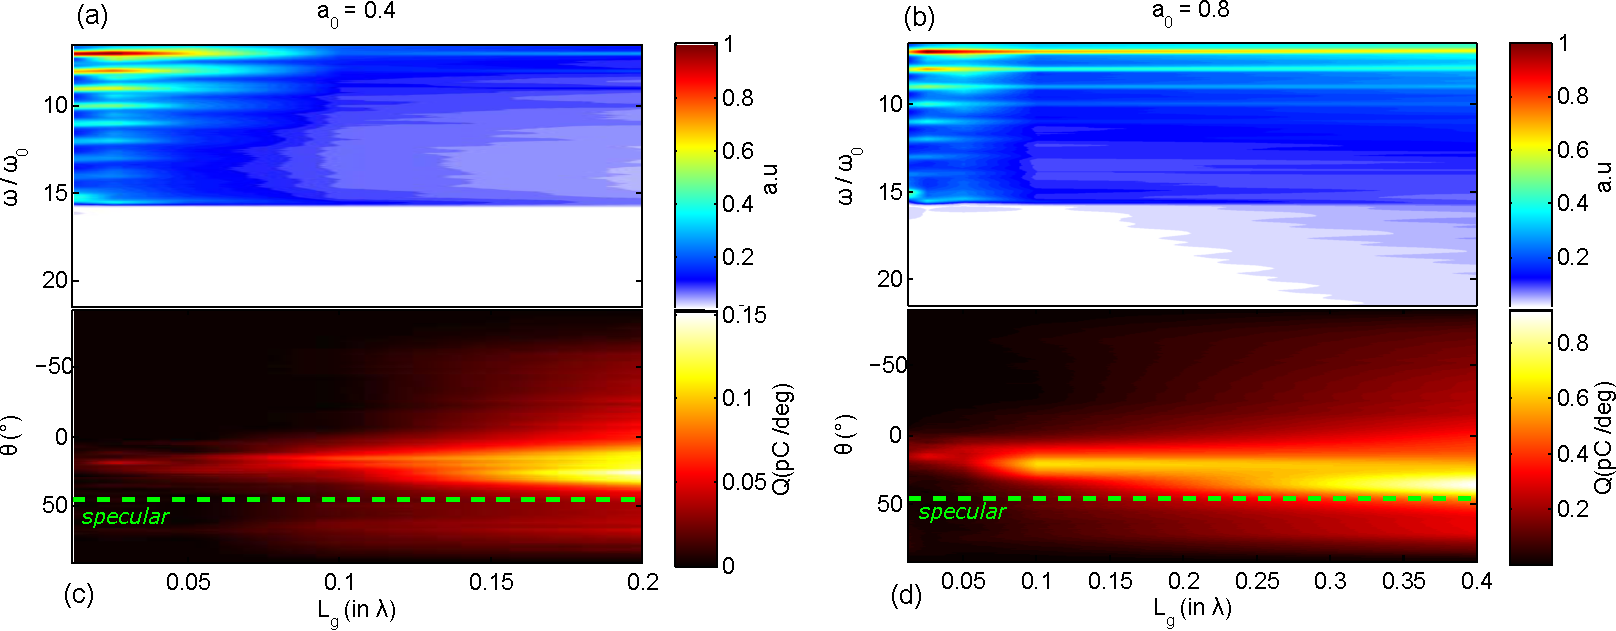
\includegraphics[width =1.3\textwidth]{../chapitre4/images/comparaionAnticorrFinal.pdf}}\\
%\captionsetup{justification=centering}
\caption{\label{fig:AntiCorrelationSimu}
2D PIC simulation using the simulation code EPOCH comparing the $a_0 = 0.4$ and $a_0 =0.8$ simulation cases. (a) and (b) HHG spectral emission integrated along its divergence as a function of initial plasma scale length. (c) and (d): electron angular emission as a function of plasma scale length. The laser specular direction at $45^{\circ}$ is indicated by the dotted green line.}
\end{figure}


\begin{figure}[H]
\begin{center}
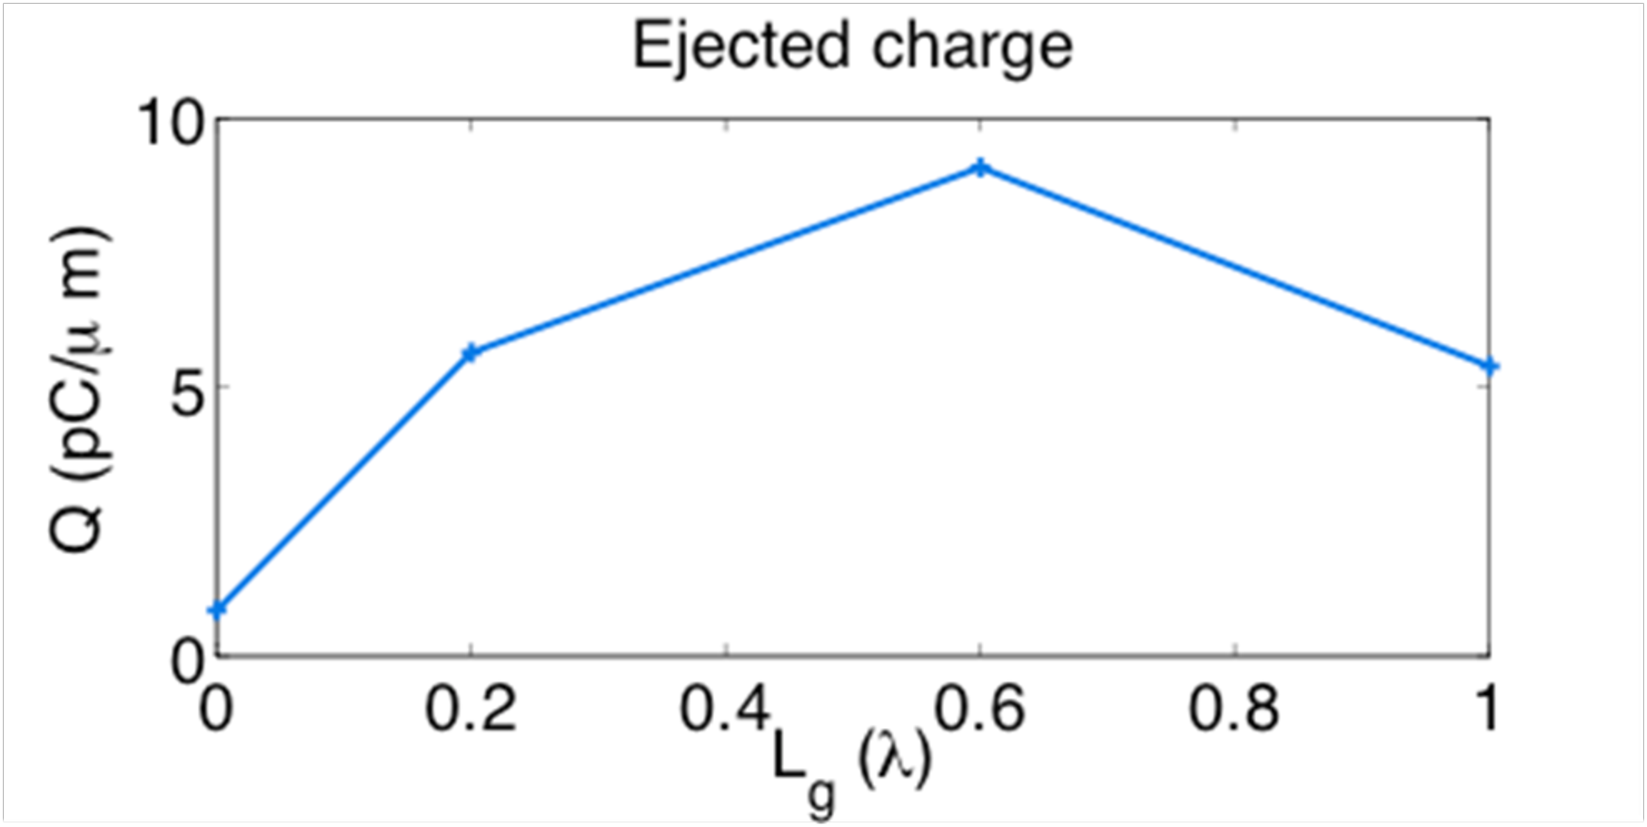
\includegraphics[width =0.7\textwidth]{../chapitre4/images/OptimumObservation_simu.pdf}
%\captionsetup{justification=centering}
\caption{\label{fig:OptimumObservation_simu}
Ejected charge retrieved from 2D PIC simulations for  density of $250n_c$ and $a_0 = 0.4$ as function of gradient scale length $L_g$}
\end{center}
\end{figure}

%
%\begin{figure}[!h]
%\centering
%\fbox{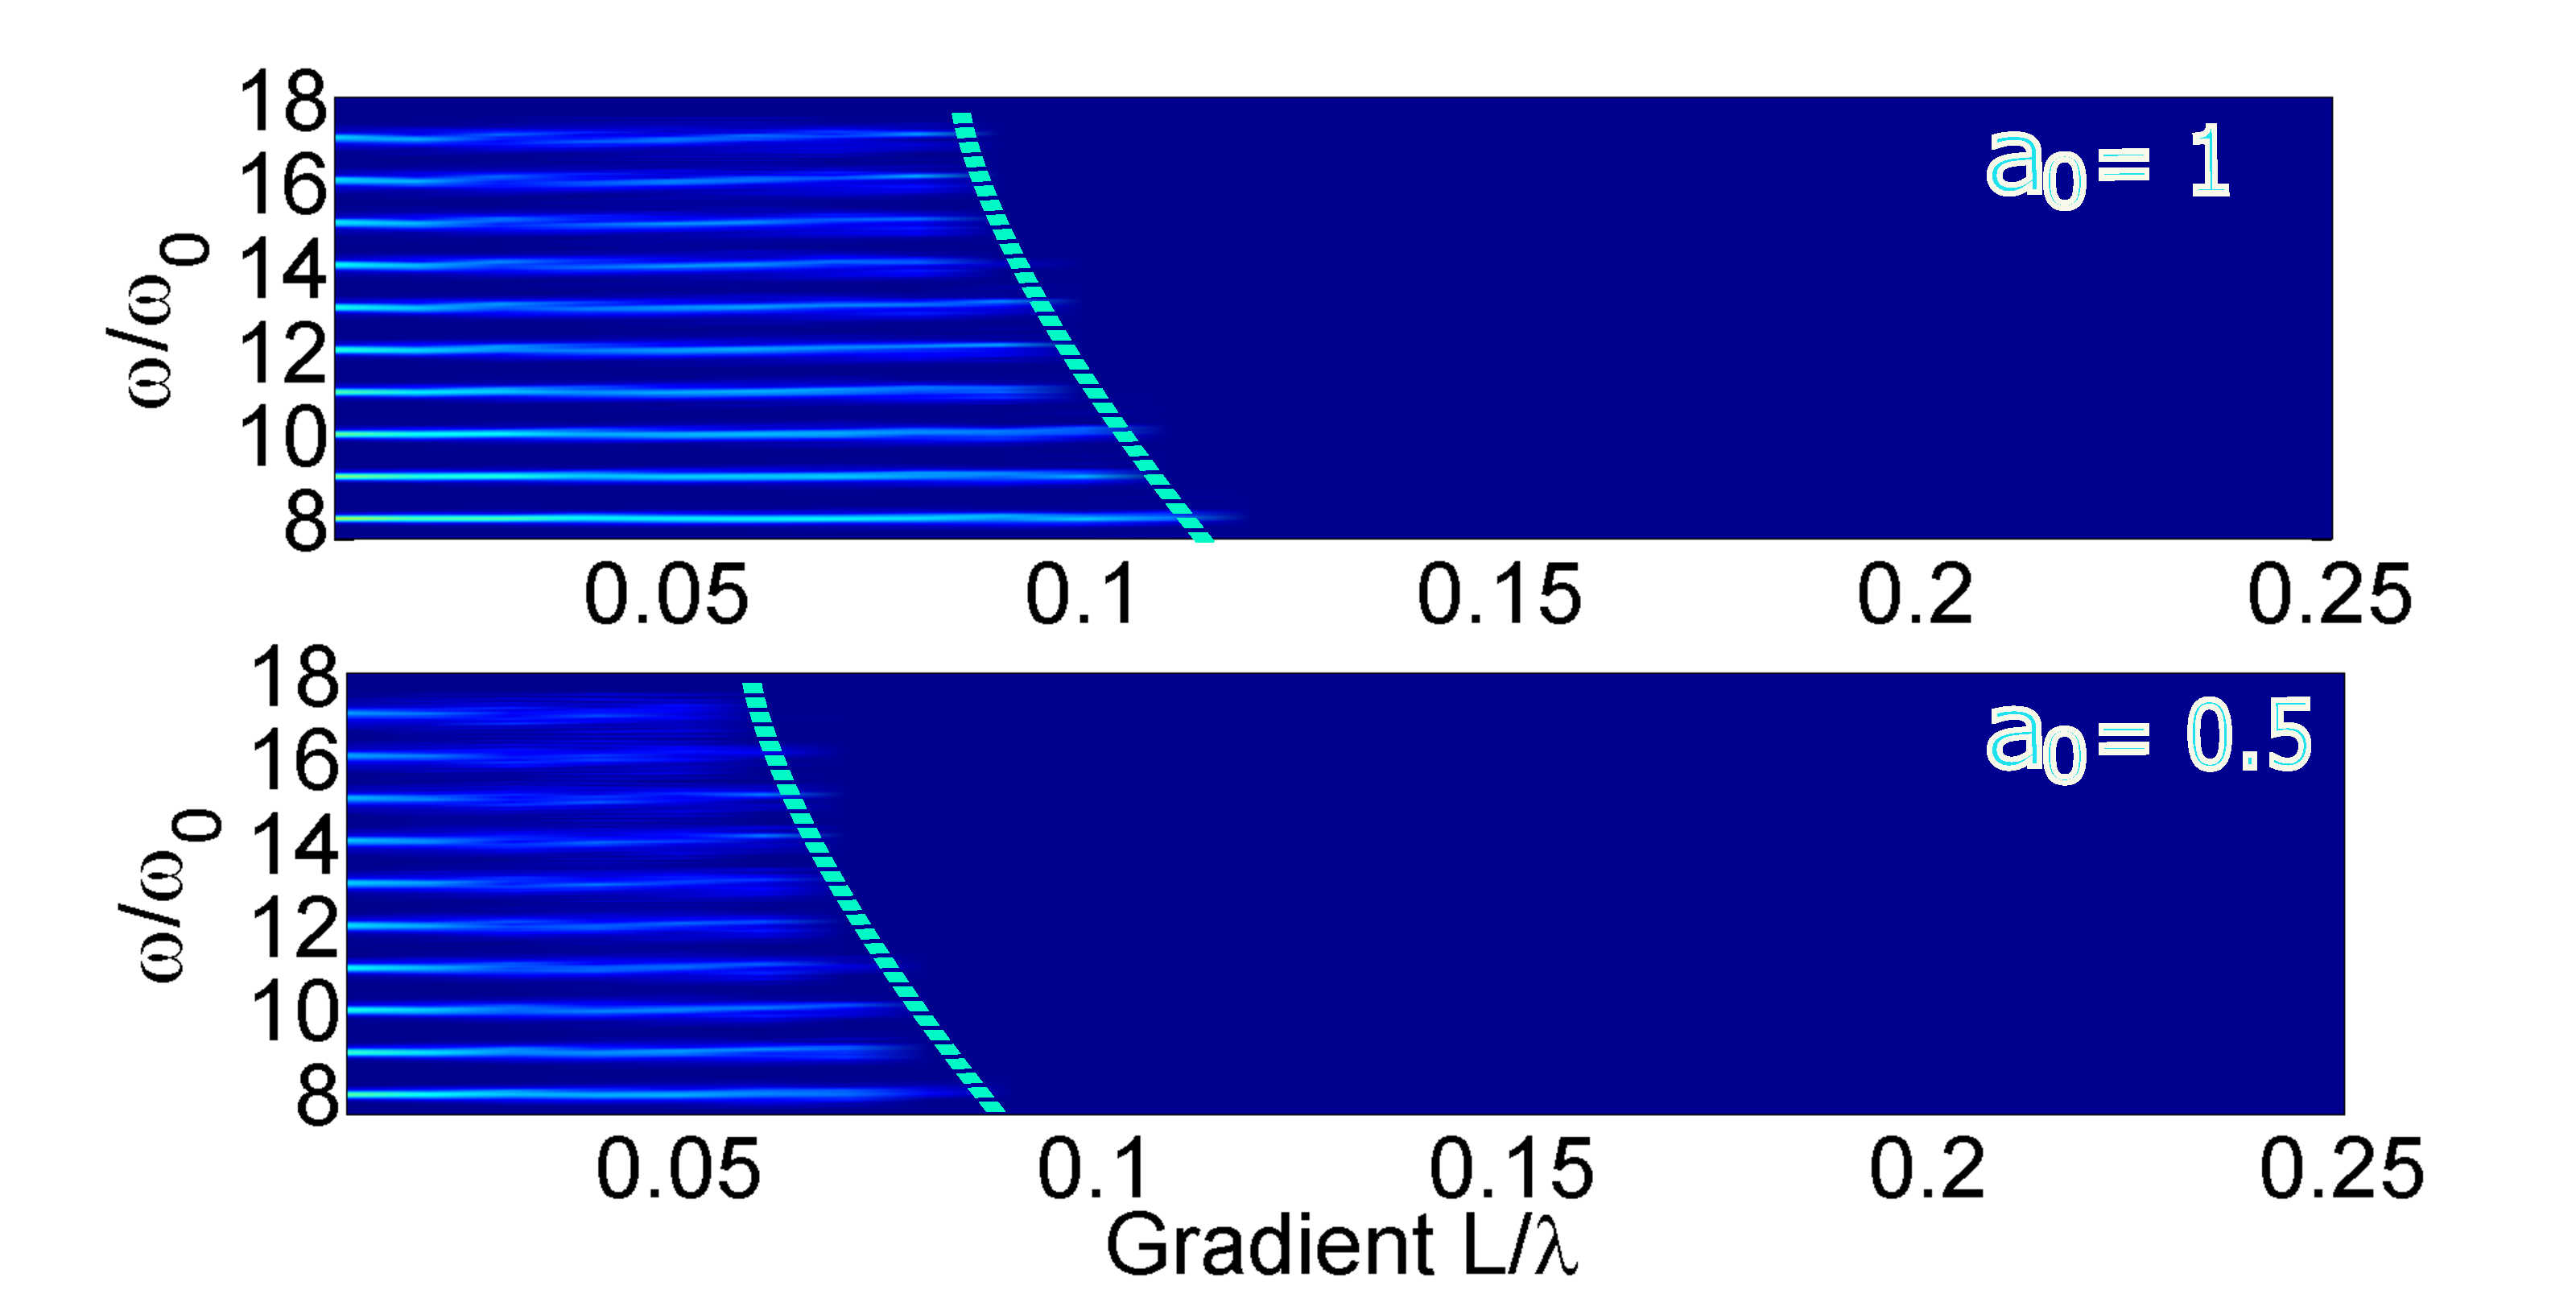
\includegraphics[width =15cm]{../chapitre1/images/CutOff_modelComparaison.pdf}}\\
%\caption{\label{fig:CutOff_modelt}1D model results for harmonic signal as a function of gradient's length for $a_0 = 1$ (top) and $a_0 = 0.5$(bottom). The gradient length cut-off decreases with the driving laser amplitude.}
%\end{figure}

\section{Electron angular emission}

\subsection{LANEX detection plane: stereographic losses}

The LANEX geometry is an important factor to consider for the deconvolution of the measured electron beam profile. We detect electrons coming from the focal spot we defined by the point $(x,y,z) = (0,0,0)$, after ballistic propagation. We define by $(x,y,z)$ a point of the LANEX detection plane $\mathcal{L}$ and express it in spherical coordinates:

\begin{equation}
\label{eq:SphericalCoord}
  \left\{
      \begin{aligned}
      & x = r\cos(\theta)\sin(\phi)\\
      & y = r\sin(\theta)\sin(\phi)\\
      & z = r\cos(\phi)\\
      \end{aligned}
    \right.
\end{equation}

\noindent For the hemisphere $\theta \in \left[ 0,\pi \right]$, $\phi \in \left[ 0,\pi \right]$ as represented in Fig~\ref{fig:SpericalRep}\\

\noindent The LANEX plane ($\mathcal{L}$) equation is:~
\begin{equation}
y = ax+b
\label{eq:LanexEq}
\end{equation}



\begin{figure}[H]
\centering
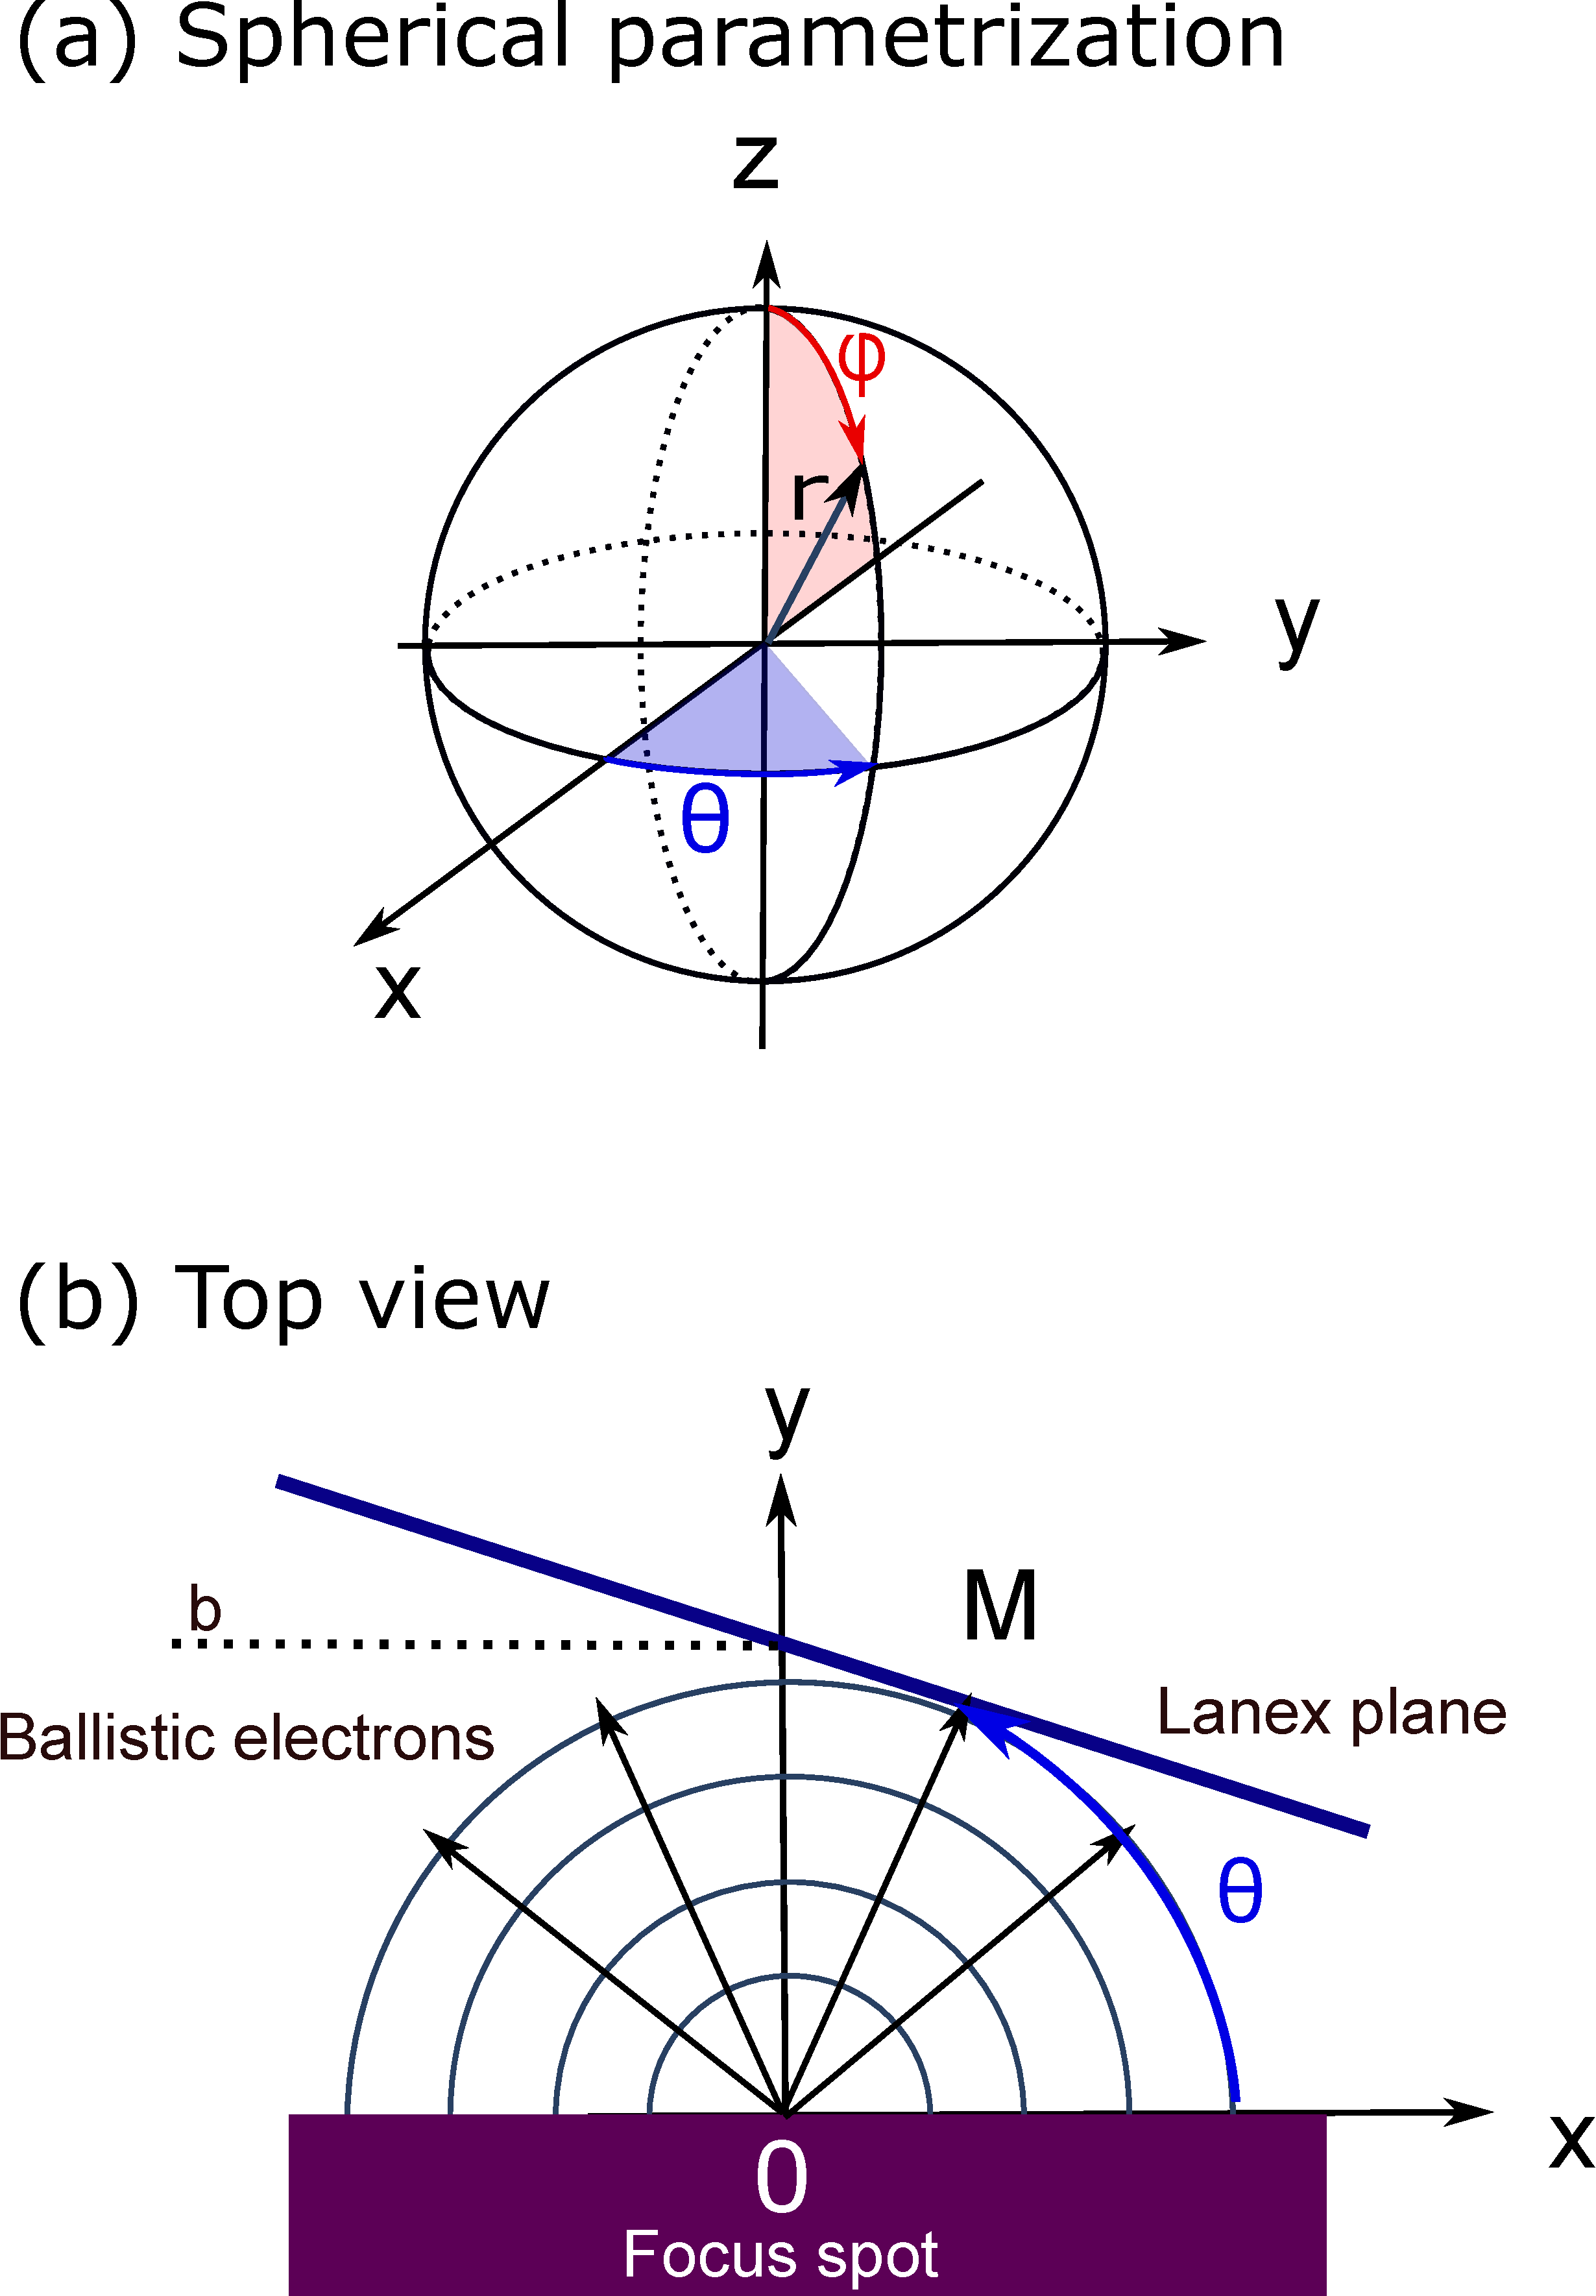
\includegraphics[width =6cm]{../chapitre4/images/SpericalRep.pdf}\\
%\captionsetup{justification=centering}
\caption{\label{fig:SpericalRep}(a) Spherical parametrization of the coordinates (b) Top view}
\end{figure}




\noindent If we consider a point $M \in \mathcal{L}$, it will verify Eq~\ref{eq:LanexEq} such that only two parameters are necessary, namely $(x,z)$  or $(\theta,\phi)$, to define its position. One can easily verify by eliminating $r$ from Eq~\ref{eq:SphericalCoord}, that they are related by the equation:

\begin{equation}
\label{eq:ChangeVar}
  \left\{
      \begin{aligned}
      & x =\frac{b}{\tan(\theta)-a}\\
      & z = \frac{b}{\tan(\phi)(\sin(\theta)-a\cos(\theta))}\\
      \end{aligned}
    \right.
\end{equation}
 
\noindent Being careful that $\theta \in \left[ 0,\arctan(a) \right[$ if $a>0$ or $\theta \in \left[ 0,\pi+\arctan(a) \right[$ if $a<0$ (our conditions) and $\phi \in \left] 0,\pi \right[$.
The signal is detected experimentally on the LANEX, however, it is the angular distribution information we are interested in. In order to derive its expression, we can write the conservation of the number $N$ of ejected electrons when switching from Cartesian to spherical coordinates:

\begin{equation}
N = \underbrace{\iint_{\mathcal{L}}n_{xz}(x,z)dxdz}_{n_{xy}[\mathrm{cm}^{-2}]}=\underbrace{\iint_{\theta,\phi}n_{\theta \phi}(\theta,\phi)\sin(\phi)d\theta d\phi}_{n_{\theta\phi}[\mathrm{sRad}]}
\end{equation}

\noindent Using~\ref{eq:ChangeVar}, we calculate the Jacobian matrix relative to the change of coordinates:

\begin{equation}
J =  \left( \begin{array}{cc}
\frac{-b}{(\sin\theta- a\cos\theta)^2} & 0\\
\partial_{\theta}[z(\theta,\phi)] & \frac{-b}{(\sin(\theta)-a\cos(\theta))\sin(\phi)^2}
\end{array} \right)
\end{equation}


\noindent With the relation $n_{xz}|\det{J}| = \sin(\phi)n_{\theta\phi}$ where "$\det$" is the determinant of $J$. We finally have:


\begin{equation}
\label{eq:ChangeNrelation}
n_{\theta\phi} = n_{xz}\frac{b^2}{\sin(\phi)^3|\sin(\theta)-a\cos(\theta)|^3}
\end{equation}

\noindent Fig~\ref{fig:LanexProjections} illustrates the geometrical projection effect on the signal recorded using the example of an isotropic emission from the target detected on a plane screen. The projected distribution is not uniform because its density increases at closer distances to the point source. Therefore, the angle of the LANEX relative to the target normal can artificially shift the measured distribution, as shown in the two image projections for a LANEX plane positioned at respectively $0^{\circ}$ (left) and $45^{\circ}$ (right) to target normal:




\begin{figure}[H]
\centering
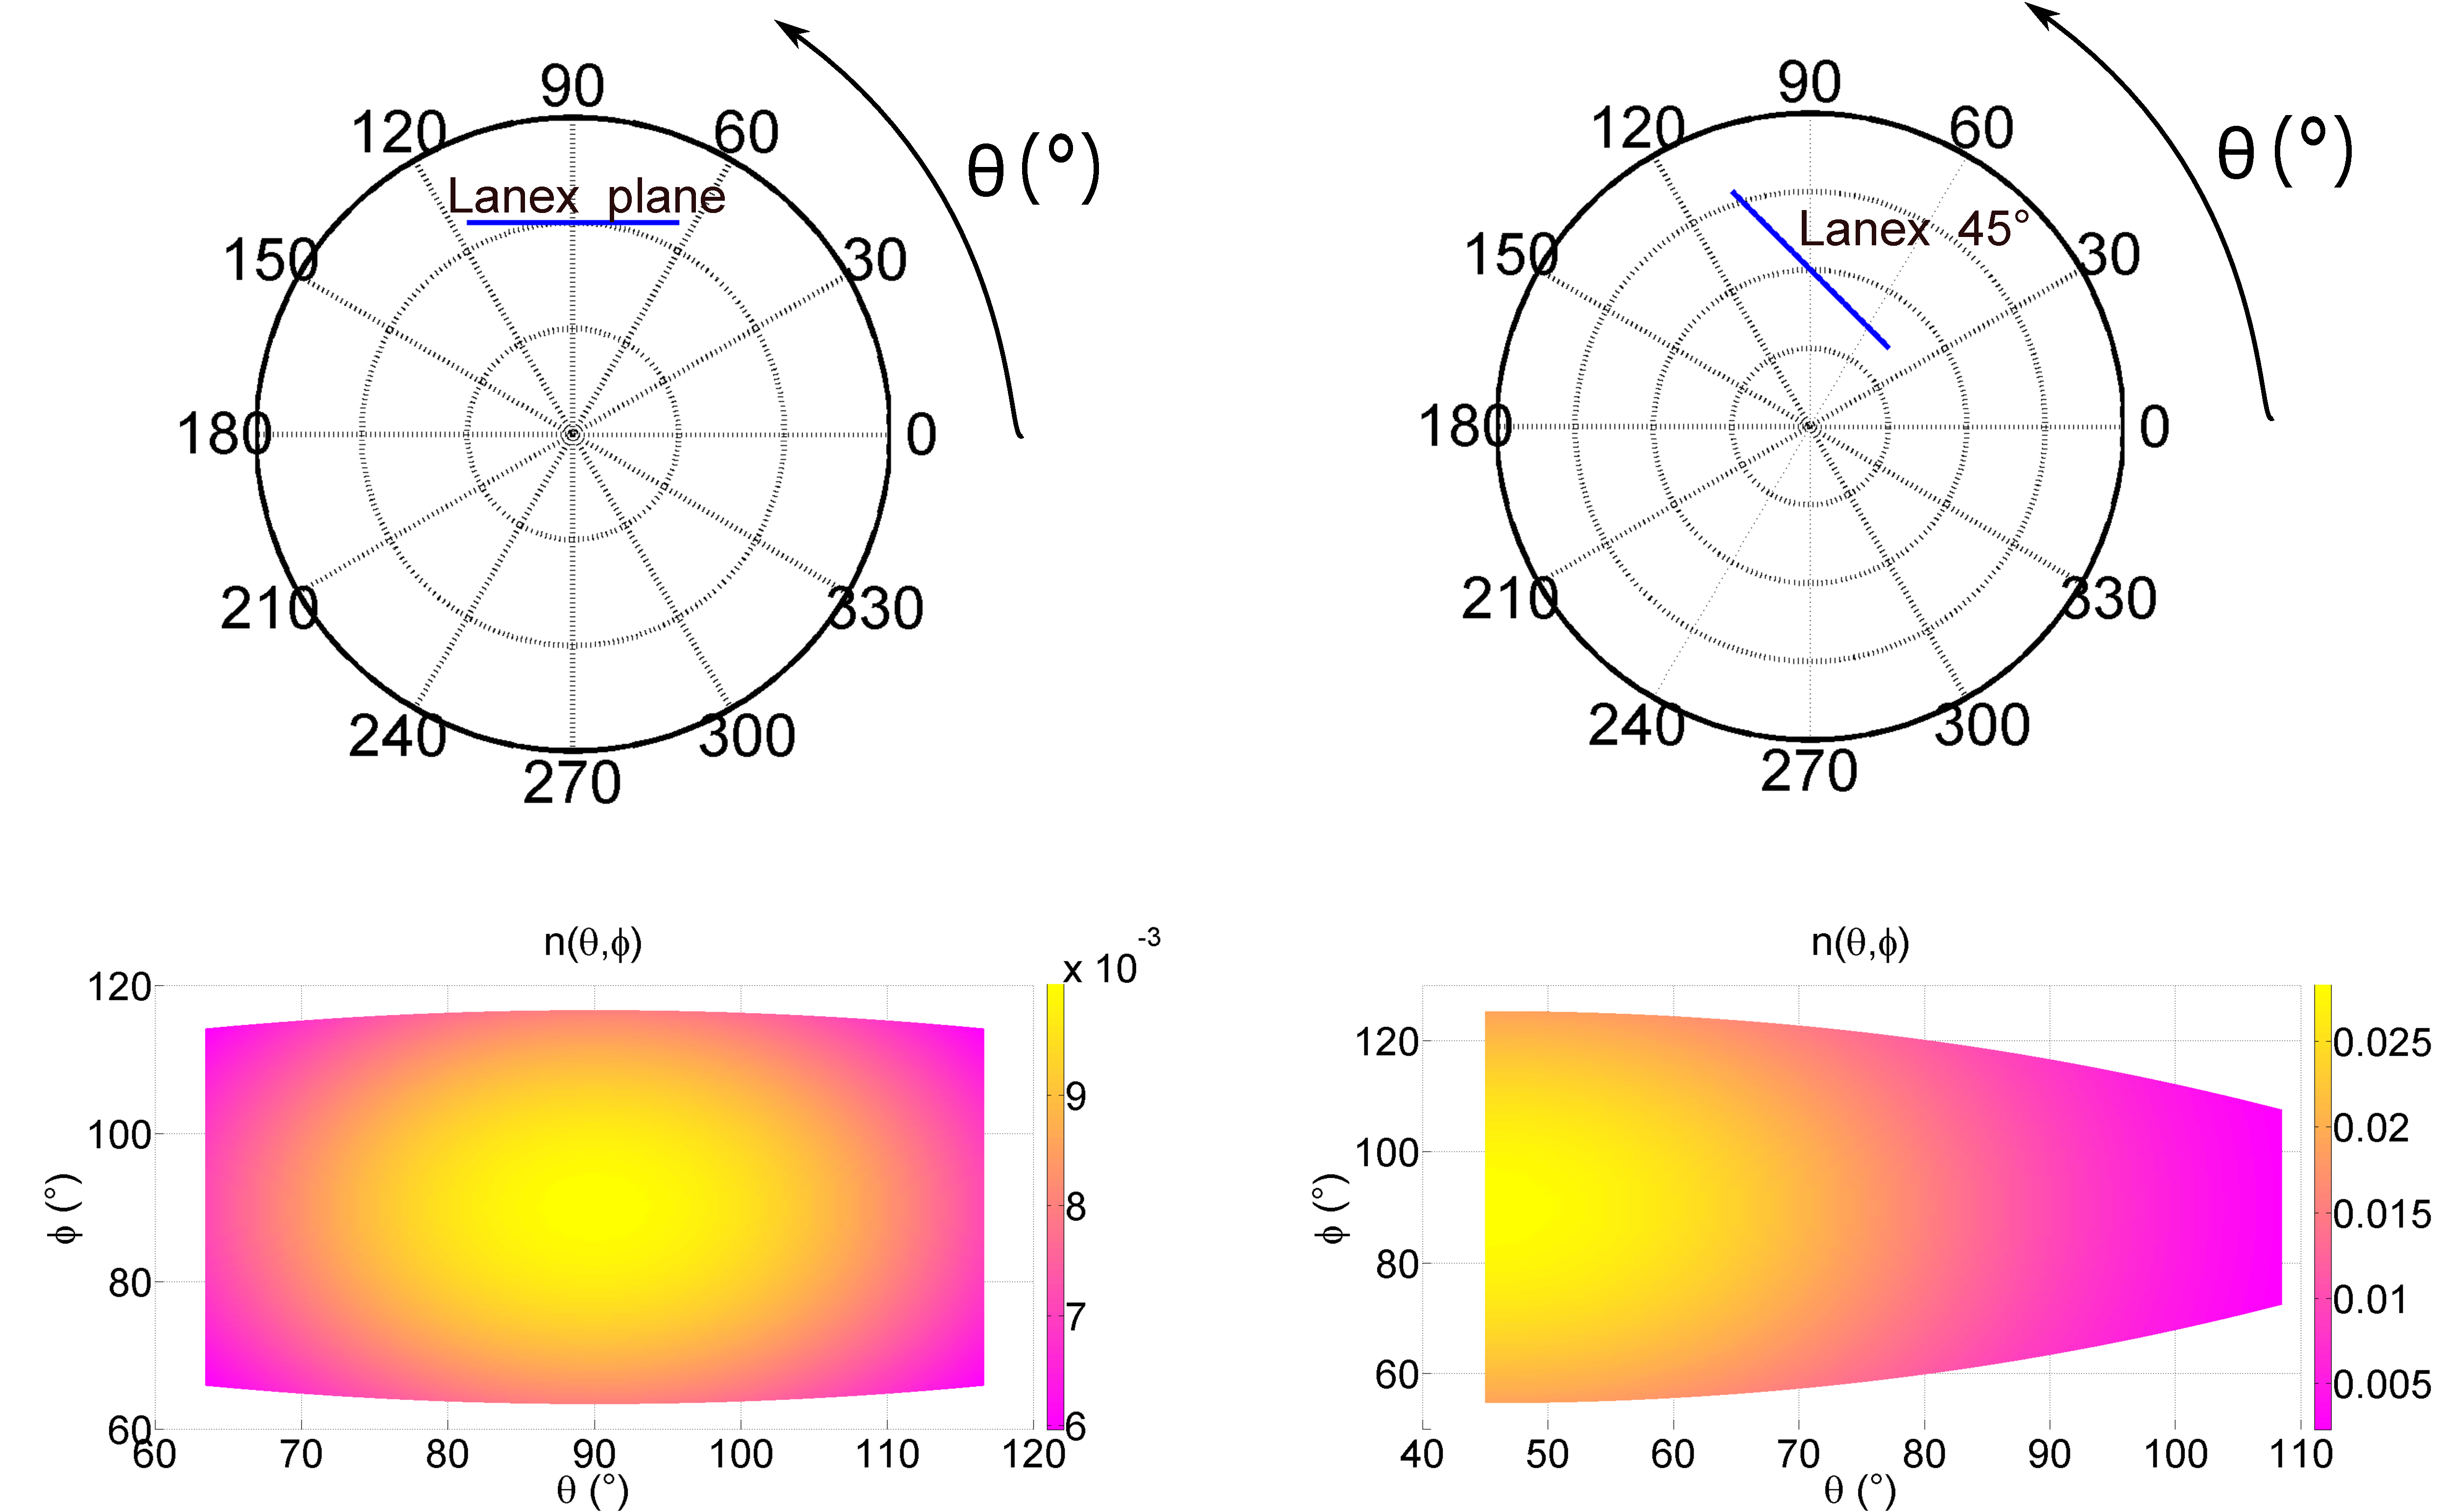
\includegraphics[width =12cm]{../chapitre4/images/SphericalProjectionExamples.pdf}\\
\caption{\label{fig:LanexProjections} Projection on the LANEX plane $\mathcal{L}$ of an isotropic ballistic emission for respectively $\mathcal{L}: y = -10$ (bottom left) and $\mathcal{L}: y = - x -10$ (bottom right) }
\end{figure}

\noindent It is therefore important to accurately measure the LANEX position $\mathcal{L}$ for proper signal deconvolution. However, this effect is of second order relative to the non-isotropic emission of the LANEX presented in the following paragraph.




\subsection{LANEX imaging: non isotropic emission losses}

An other element to take into account in the electron signal deconvolution is the anisotropic emission of the LANEX which is known to be Lambertian, that is to say $\propto \cos(\alpha)$ \cite{glinec2006absolute}, where $\alpha$ is the angle to the normal direction. This means that the LANEX fluorescence reaching the camera objective at high incident angles is hardly detected. To calibrate this response $R$, we translated the camera along the plane  $\mathcal{L}$ defined by the LANEX and recorded the signal intensity distribution, shown in Fig~\ref{fig:DeconvoTranslationLANEX}(c). For each position, the integrated signal on camera is given by Eq~\ref{eq:lanexrespondTrans}:
\begin{equation}
\label{eq:lanexrespondTrans}
S_{\text{CCD}}(x) = R(x)S(x-\Delta x)
\end{equation}


\begin{figure}[H]
\centering
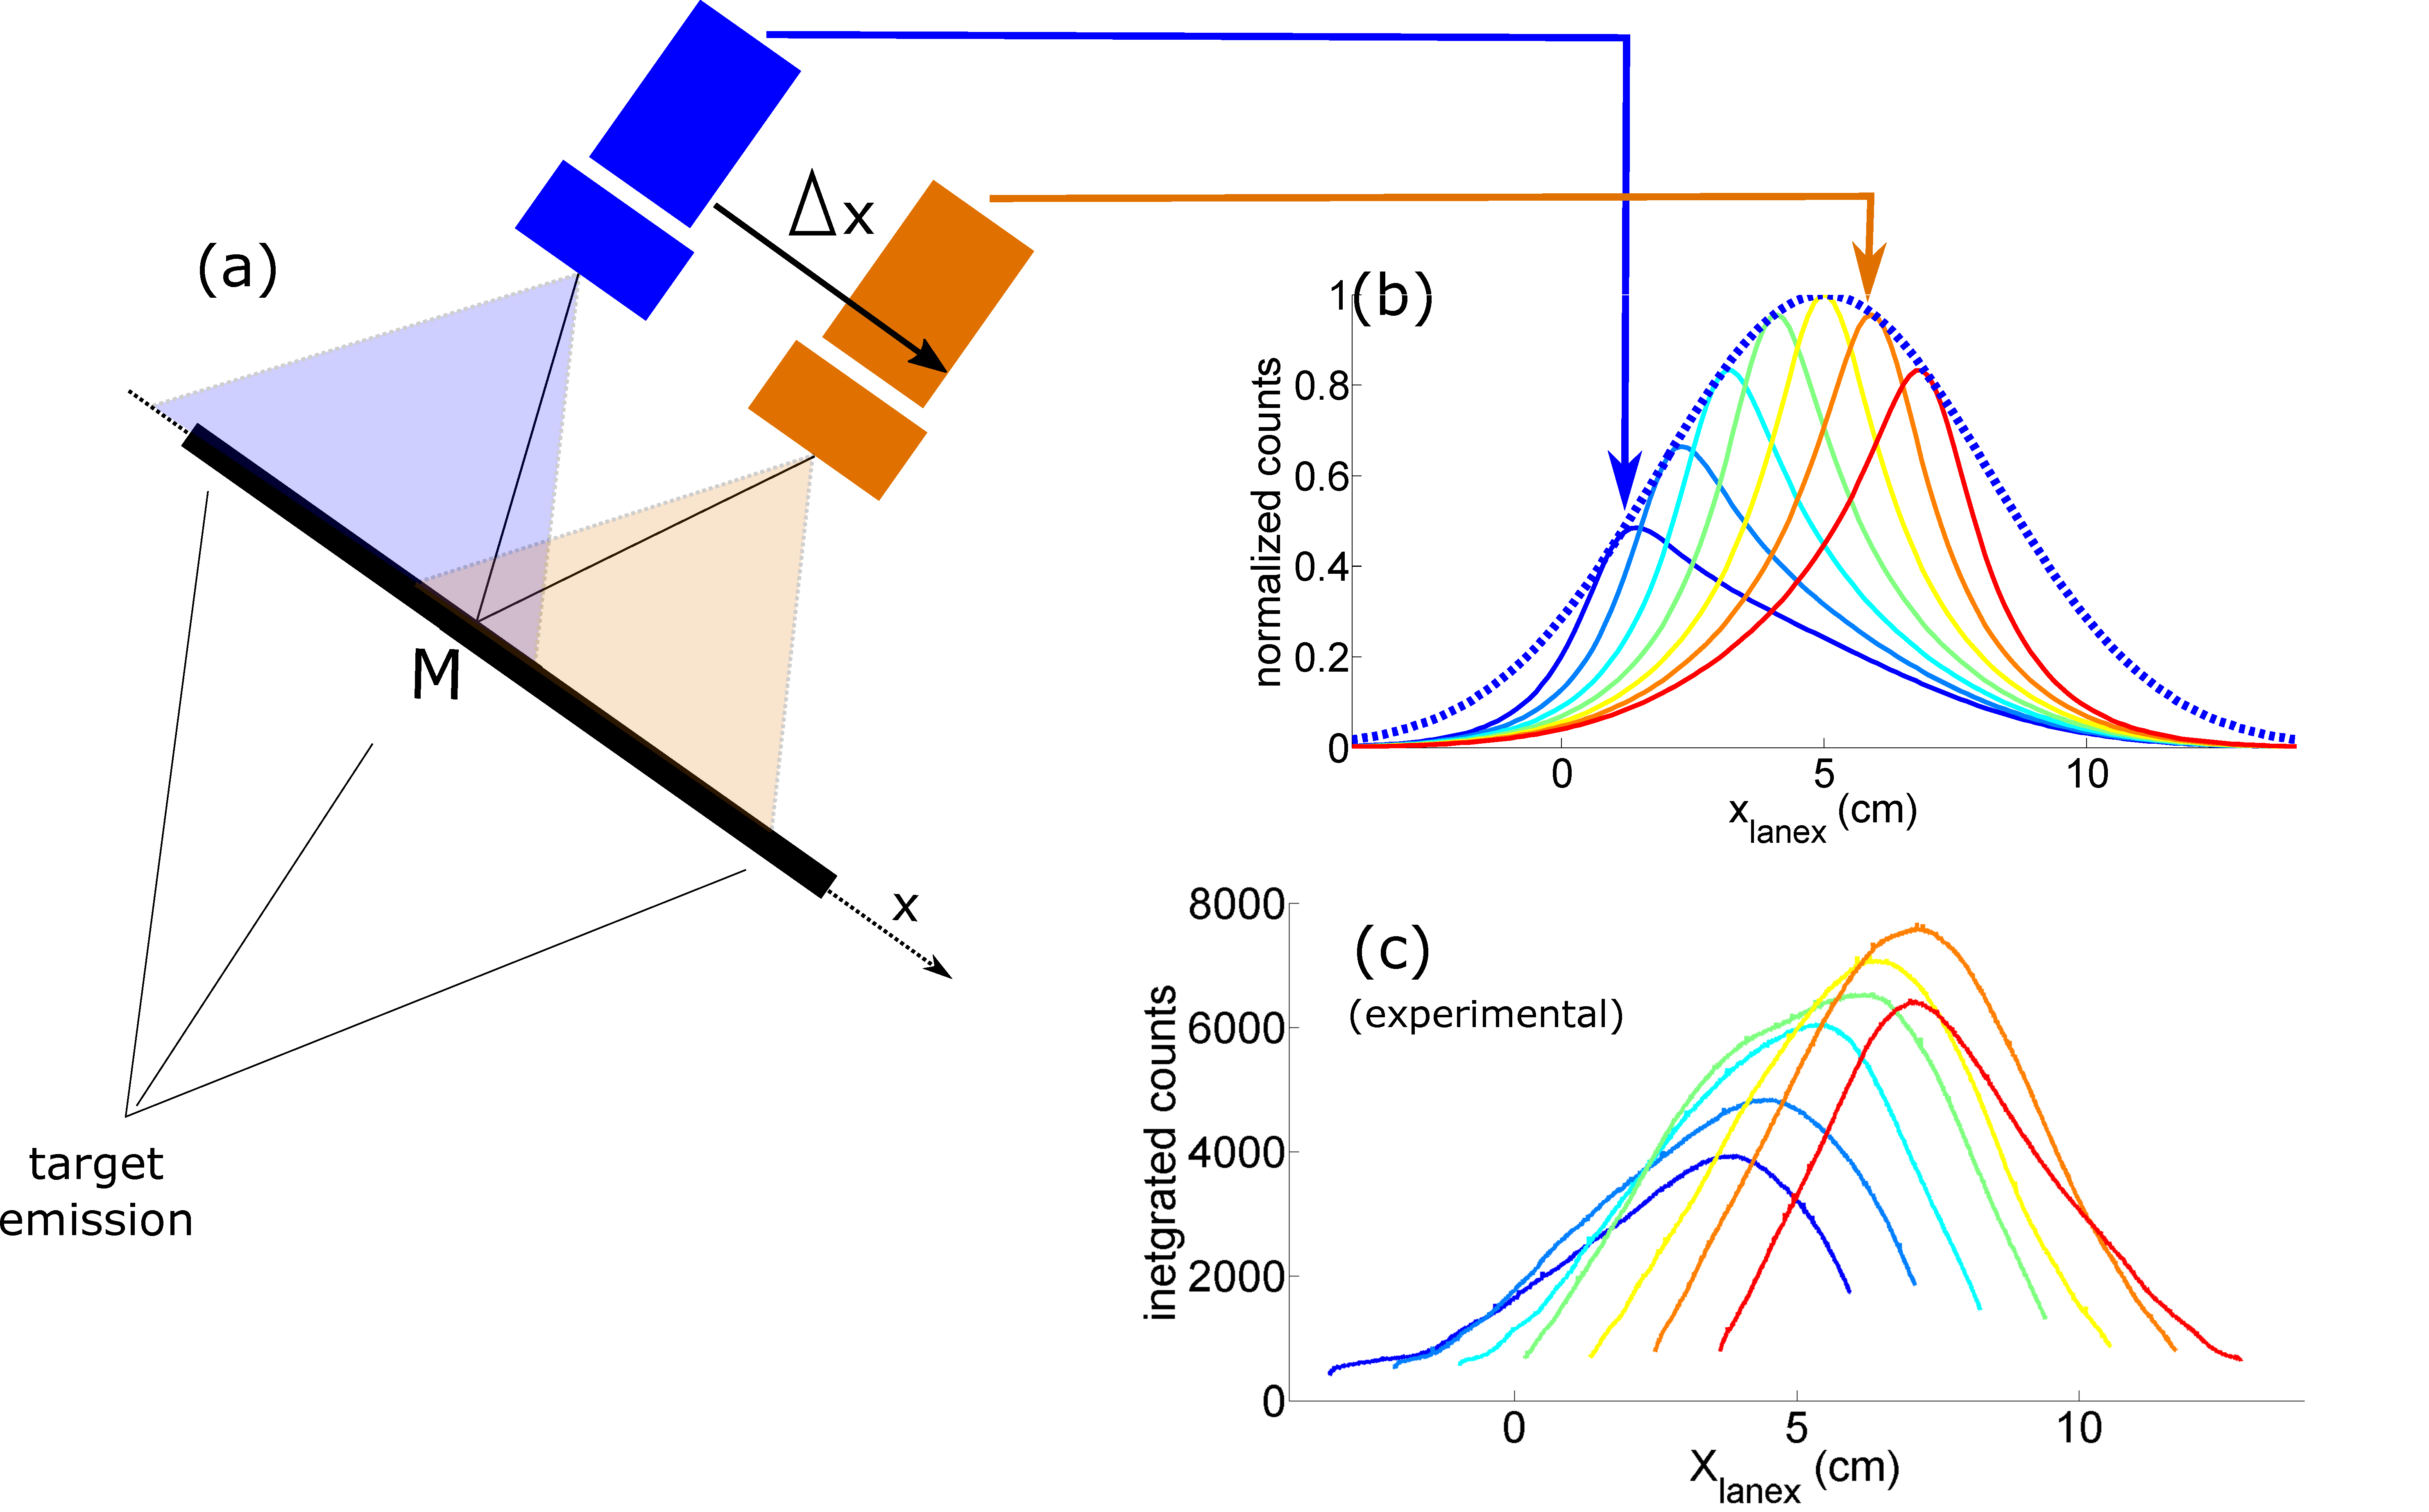
\includegraphics[width =15cm]{../chapitre4/images/DeconvoTranslationLANEX.pdf}\\
\caption{\label{fig:DeconvoTranslationLANEX} (a) Layout of the experiment: the electron signal is recorded along a given plane for different positions of the CCD (illustrated by blue and orange colors). (b) Simulation of the effect due to LANEX Lambertian emission. A Gaussian distribution is represented by the dotted line. Each successive color lines correspond to this signal intensity for a displacement of $\Delta x$. Each color corresponds to a displacement of 1cm. (c) Experimental results obtained by translating the LANEX along $\mathcal{L}: y = -0.46 x + 10\mathrm{(cm)}$ as a comparison. CCD counts are integrated in the vertical direction.}
\end{figure}



\noindent where $S$ is the electron signal on the LANEX, $R$ the response to due to anisotropic emission and $\Delta x$ is the value to which the camera has been translated. For a given displacement $\Delta x$, the maximum signal $S_{\text{CCD}}$ is obtained when two conditions are met: (i) $S(x-\Delta x)$ is maximal and (ii) the LANEX response is maximal $R(x) = 1$.
This can be visualized in Fig~\ref{fig:DeconvoTranslationLANEX}. As a consequence, the curve represented by $S$ will always be tangent to the measurement $S_{\text{CCD}}$ every time $R = 1$. We use this property to sample the signal at 7 different positions. Moreover, we consider that the measured signal gives us no information when it is just within the background noise. The result of the LANEX response reconstruction is give in Fig~\ref{fig:DeconvoLANEX-fit}. We find that the LANEX response can be fitted with a polynomial function of fourth order centered around the optical axis of the imaging system. The deviation from a Lambertian emission profile is certainly due to the convolution with the imaging objective of the camera.\\



%(..). We then fitted the result of the deconvolution with a polynomial function giving as a result: 
%
%\begin{equation}
%R(x) = -0.0004 +   0.0004 x   - 0.0279  x^2 +  0.0006 x^3 +  1.0098 x^4
%\end{equation}*
%



\begin{figure}[H]
\centering
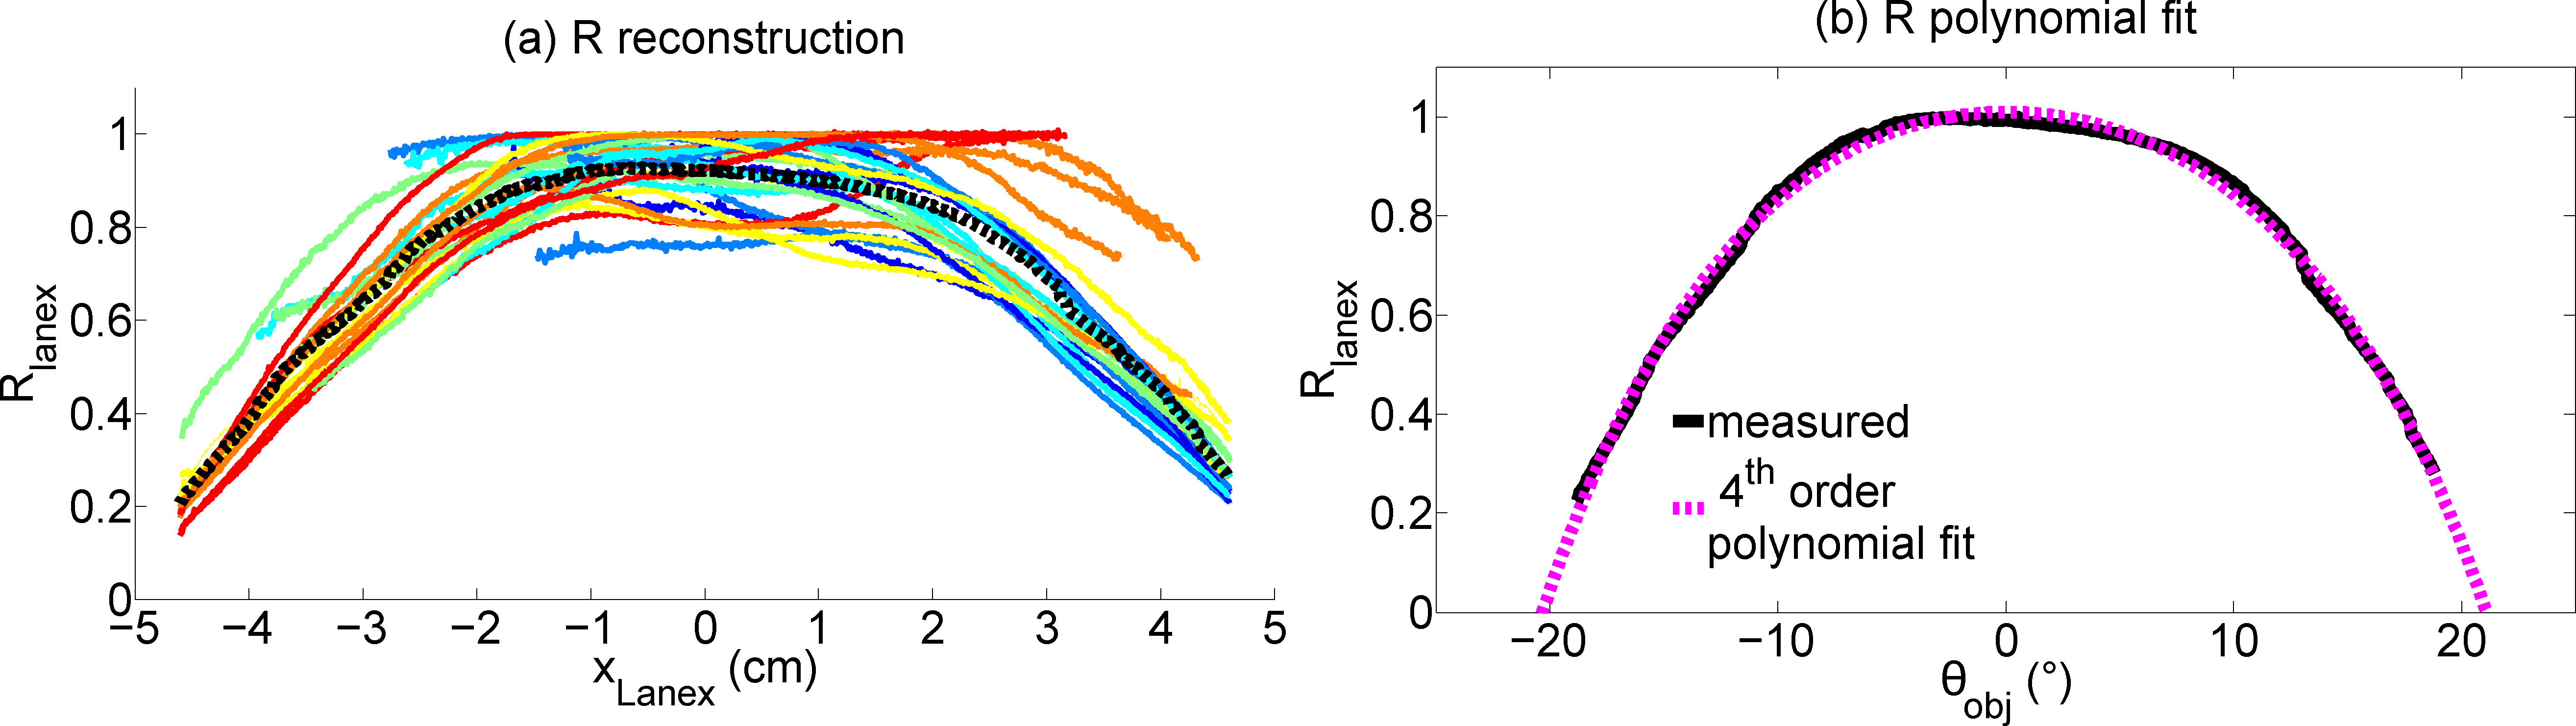
\includegraphics[width =\textwidth]{../chapitre4/images/LanexResponseDec.pdf}\\
\caption{\label{fig:DeconvoLANEX-fit} (a) R reconstruction: average over 20 sequences of 100 shots each (b) Corresponding polynomial fit of LANEX response as a function of incident angle on camera objective} %. $S_{camera} < S_{camera,max}/10$ are not considered because of noise level
\end{figure}

% distance objective-lanex = 13cm

\g{Consequences:}\\

\noindent We already mentioned the discrepancies between the electron average angle of emission in experiment and simulations when the LANEX is normal to the target. We just described how geometrical projections and non-isotropic emission are responsible for signal losses. Deconvolution of a signal within the camera noise limit does not make sense, which is why we say the signal is "lost". We illustrate this effect by recording the electron profile when the LANEX is placed normal to the specular direction in Fig~\ref{fig:EffectOfProjection}.


\begin{figure}[H]
\centering
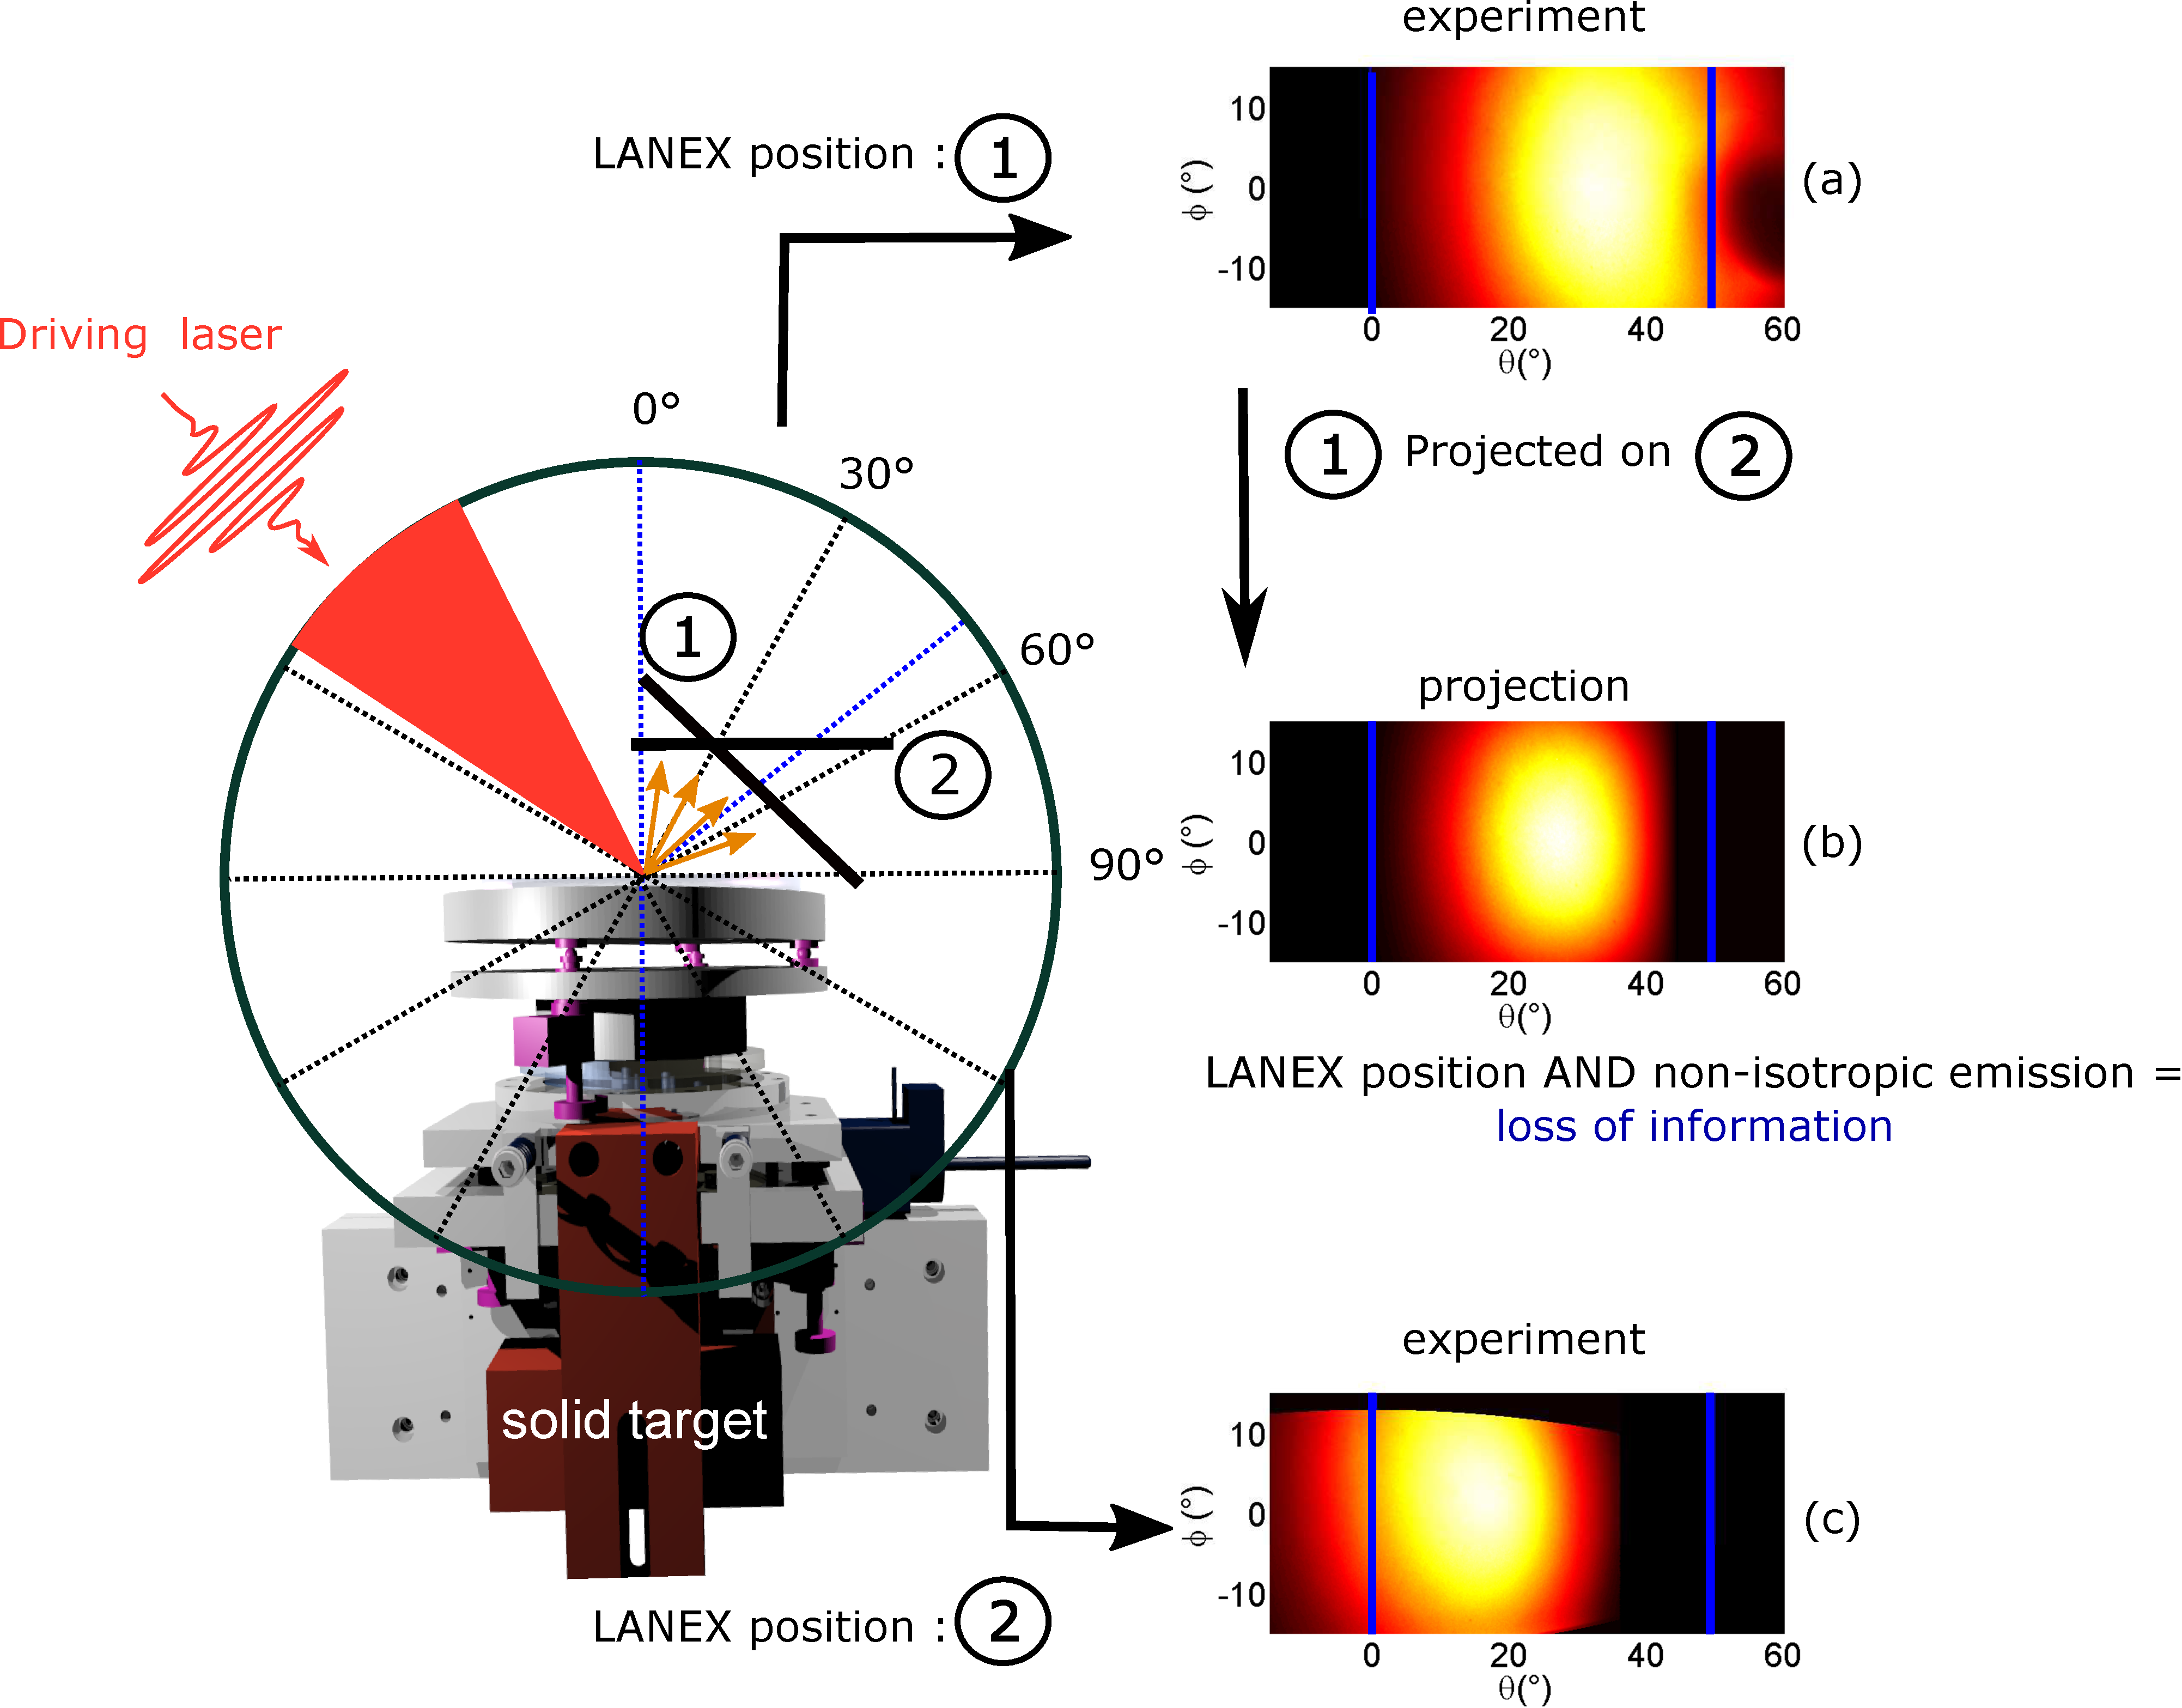
\includegraphics[width =\textwidth]{../chapitre4/images/EffectOfProjection.pdf}\\
\caption{\label{fig:EffectOfProjection} Projection on the LANEX (indicated with black solid line) of the electron angular distribution. One can clearly see the loss of information due to the geometrical position of the LANEX and its non-isotropic emission response}
\end{figure}

%\subsection{Number of electrons deconvolution}
%
%In order to record the full electron profile from the target, we installed the latex screen on a translation stage under vacuum as described in the following experimental scheme. 
%We define $n_{\theta\phi}$ as the ejection angular distribution. Note here that the orthoradial space charge effect occurring at distances much greater than the Rayleigh length is completely neglected. The phosphor signal is recorded with a PL-B957U, 10bit Pixelink Camera with a $1392\times 1040$ resolution chip with squared $6.45\mathrm{\mu m}$ pixels. We have calibrated this camera conversion efficiency and measured 
%$$
%N_{c/e^{-}} = 6 \mathrm{electrons/counts}
%$$
%
%The camera was mounted with a H1212B elvitech camera objective if $12$mm focal.

\newpage
\subsection{Spatial distribution of ejected electrons}\label{subsub:Spatial distribution of ejected electrons}

%

The angle at which electrons are ejected from a solid target is subject to debate. Experimental results for a laser intensity of $a_0 \sim 1$ \cite{mordovanakis2009quasimonoenergetic} suggest electrons are ejected around 34° from the target normal with an angular divergence on the order of 10°. Another experiment where $a_0\sim0.13$ \cite{bastiani1997experimental} hints towards highly collimated beams ($\sim 3$° divergence ) in the specular direction, while other experiment for long gradient demonstrate  normal~\cite{li2001hot} or grazing acceleration~\cite{chen2006surface,li2006observation}. The diversity of these results highlights the importance of the  interaction parameters, namely the intensity on target and the gradient scale length. 
If providing a highly collimated and monoenergetic electron is the long-term objective, the priority so far is to understand the close correlations between the emission profile and spectral distribution of electrons with respect to the gradient scale length and laser intensity.\\



\begin{figure}[H]
\begin{center}
\makebox[\textwidth][c]{
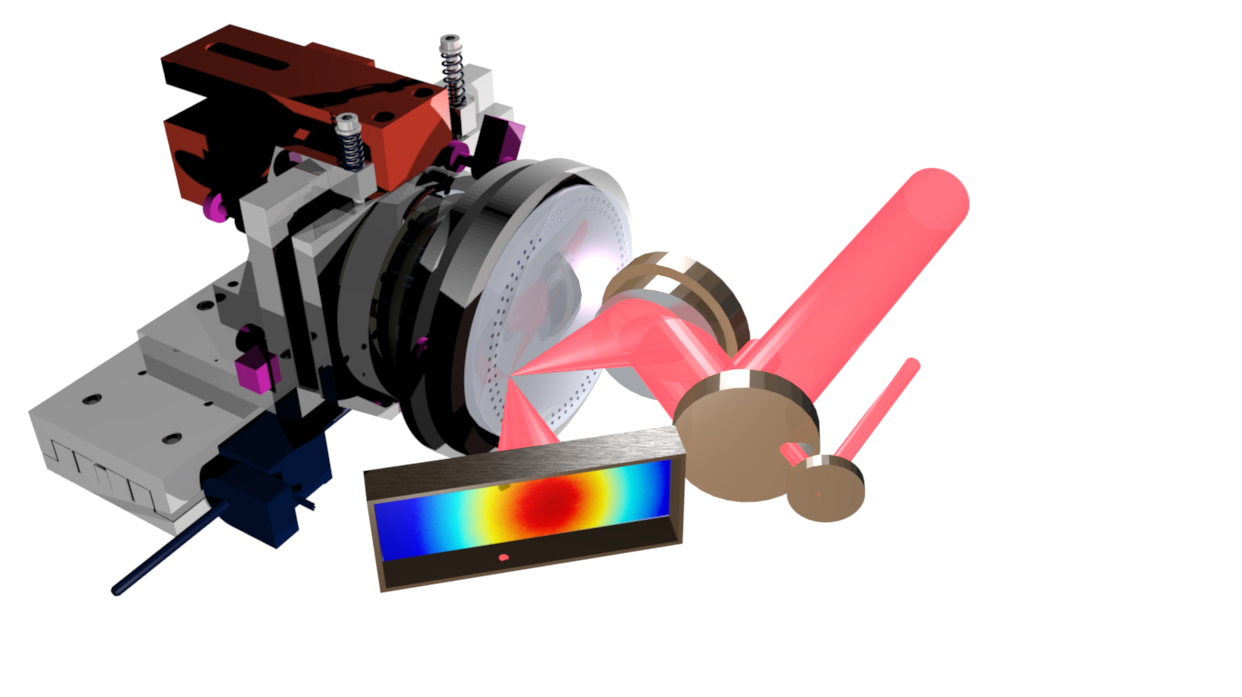
\includegraphics[width =0.9\textwidth]{../chapitre4/images/ElectronNormalSpecular.png}}
\caption{\label{fig:ElectronNormalSpecular}Experimental setup for electron detection in the specular direction. Prepulse: $I \sim 10^{14}\,\mathrm{W/cm^2}$ and main pulse: $I\sim 10^{18}\,\mathrm{W/cm^2}$. The laser incidence angle is $50^{\circ}$.} 
\end{center}
\end{figure}

\noindent In the previous results, we detected electrons ejected $\sim 16^{\circ}$, but mostly because the LANEX used for detection was positioned normal to the target. In the following experiment, we  position the LANEX normal to the specular direction to recover the full angular emission profile of ejected electrons as represented in Fig~\ref{fig:EffectOfProjection}, thereby obstructing HHG detection. We now discuss the underlying mechanisms of electron acceleration and ejection from an overdense plasma target, at subrelativistic intensities and for $L<\lambda$. \\


\g{Importance of laser contrast:}\\

\noindent We have already discussed the importance of the plasma scale length during the interaction, and illustrated this statement with the experimental results presented in~\ref{section:Simultaneous HHG and electron detection}. In Fig~\ref{fig:XPW_29fs}, we can clearly see the influence of the laser contrast on the electron emission profile by changing the output angle $\alpha$ of the XPW polarizer (description in section~\ref{subsection:XPW contrast cleaning}). When the angle is large enough, that is to say $\alpha >2^{\circ}$, the contrast is degraded on the nanosecond time scale, which means that we are in presence of a very long gradient scale length. As a result, electrons are ejected closer to target normal and their profile is more chaotic. On the other hand, as we saw in Section~\ref{chapter:Overall presentation of the laser system}-~\ref{subsection:XPW contrast cleaning}, there exists a range of XPW polarizer angles between $-3^{\circ}\le \alpha \le1^{\circ}$ where only the coherent contrast is altered. In this case, the plasma scale length does  not vary significantly and neither does the electron emission profile.\\

\g{Hole in angular emission profile:}\\

\noindent Within this range, we can clearly identify in Fig~\ref{fig:XPW_29fs}, the edges of a ponderomotive "hole" formed by the laser on the right side of the specular direction (indicated by a solid black line). Its size is nearly half that of the laser divergence ($\sim 25^{\circ}$ based on geometrical considerations). The presence of such a ponderomotive hole has already been reported in literature~\cite{Wang2010,mordovanakis2009quasimonoenergetic,tian2012electron,thevenet2015}. It is attributed to the ponderomotive force~\cite{mordovanakis2009quasimonoenergetic} and systematically measured in the specular direction~\cite{thevenet2015,mordovanakis2009quasimonoenergetic}, except in~\cite{Wang2010} where the hole is formed to the side of the specular direction, however no comment is made on the matter by the authors. However, we notice that in~\cite{mordovanakis2009quasimonoenergetic}, the result of a 2D PIC simulation (showing the angular energy distribution of ejected electrons for $L= \lambda/5$ and $a_0 = 1$), the "hole" is also located on the side of the specular direction (towards grazing incidence). Again, no comment is made by the authors on the matter. In Fig~\ref{fig:XPW_29fs}, our experimental data clearly indicate that the hole is not formed in the specular direction, but at larger angles (toward grazing incidence). This peculiar effect will be investigated in future experiments. One possible explanation is that we are not exactly at focus on the target plane. In Fig~\ref{fig:XPW_29fs}, the hole is located on the right side of the specular direction as already mentioned. By translating the focusing parabola, we will see (Fig~\ref{fig:FocusScan}) that it is possible to shift the position of the hole closer to the specular direction. However, the specular direction is never reached, and a "depletion" line appears when we are in focus. This will be discussed further in~\ref{sub:Influence of non axisymmetrical component of the interference field} \\

\g{Hole disappearance with plasma expansion:}\\

\noindent  In Fig~\ref{fig:FocusDelay23fs_XPW279}, we represent the electron angular emission profile when varying the pump-probe delay from $0\,\mathrm{ps}$ to $20\,\mathrm{ps}$, which corresponds to plasma gradients between $L\sim \lambda/100$ and $\sim \lambda/2$. As expected, there is an increase of the ejected charge with increasing pump-probe delay, reaching an optimal of $\sim17\,\mathrm{pC}$ for $6\,\mathrm{ps}$ delay, which is consistent with our previous results. In addition, three remarks can be made on the profile evolution:

\begin{itemize}
\item[$\bullet$]  For short delays, the electron angular distribution shows a symmetry with respect to the plane of polarization. In addition, there is a small collimated electron spot near the ponderomotive hole formed by the reflected laser. This pattern is highly reproducible as shown by the 4 consecutive first images, and vanishes after $2$ps. We attribute this spot to non-ponderomotive laser acceleration in vacuum, as described in~\ref{subsub:Non ponderomotive laser acceleration}. This effect is much clearer at relativistic intensities~\cite{thevenet2015}, and might  explain why some authors have observed "highly collimated electron beams" in laser plasma acceleration experiments performed at subrelativistic intensities~\cite{bastiani1997experimental}.
\item[$\bullet$]  As the gradient expands, the hole formation is purely ponderomotive and gets smaller in size. This is consistent with a strong contribution of the plasma to electron acceleration.
\item[$\bullet$]  Finally, for long gradient scale lengths, the ponderomotive hole vanishes, and simultaneously the ejected charge drops.
\end{itemize}

\begin{figure}[H]
\centering
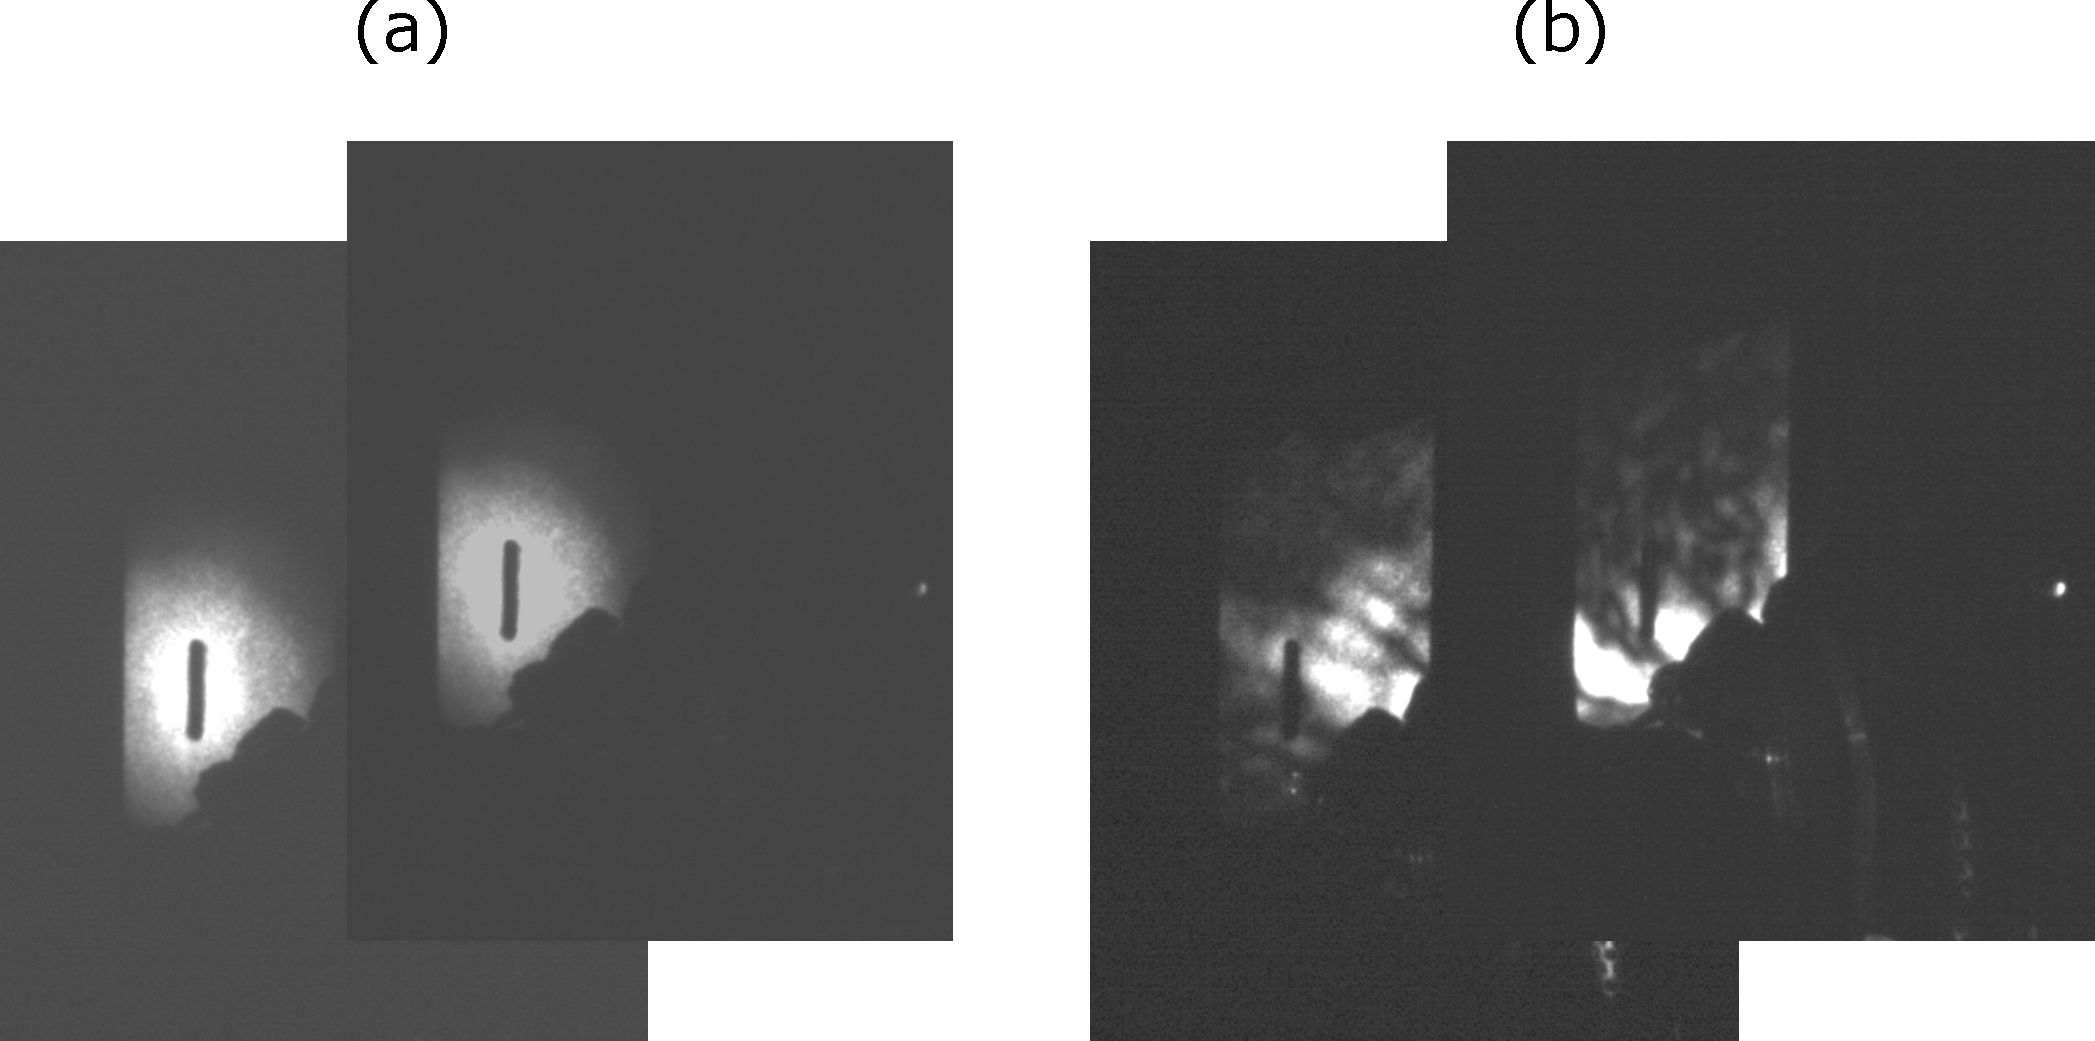
\includegraphics[width =0.7\textwidth]{../chapitre4/images/phaseDist_slit.pdf}\\
\caption{\label{fig:phaseDist_slit}Image of HHG entrance slit with (a) or without (b) prepulse}
\end{figure}


\noindent Still invoking~\cite{mordovanakis2009quasimonoenergetic}, the disappearance of the ponderomotive hole from $\lambda/5$ to $\lambda/2$ can be reproduced with PIC simulations. If the hole disappears for long gradients, then either (i) the reflected laser does not overlap with the electrons or (ii) the electrons no longer see ponderomotive effects because of their high propagation velocity. If (ii) were true, we would expect to see a significant increase of electron energy with gradient scale length. This is not the case as shown in~\ref{subsub:Spectral measurement}, where no significant variation of the spectra is observe at long gradient lengths. Moreover, for a pump-probe delay where the maximum ejected charge is reached, the ponderomotive hole is still clearly visible on the LANEX. Therefore, the disappearance of the hole should be due to (i). As shown in Fig~\ref{fig:phaseDist_slit}, the intensity profile of the laser gets distorted as the plasma expands and therefore, it becomes difficult to identify a "beam". This is consistent with the highly perturbed emission profile of the electrons for long gradients.




\begin{figure}[H]
\centering
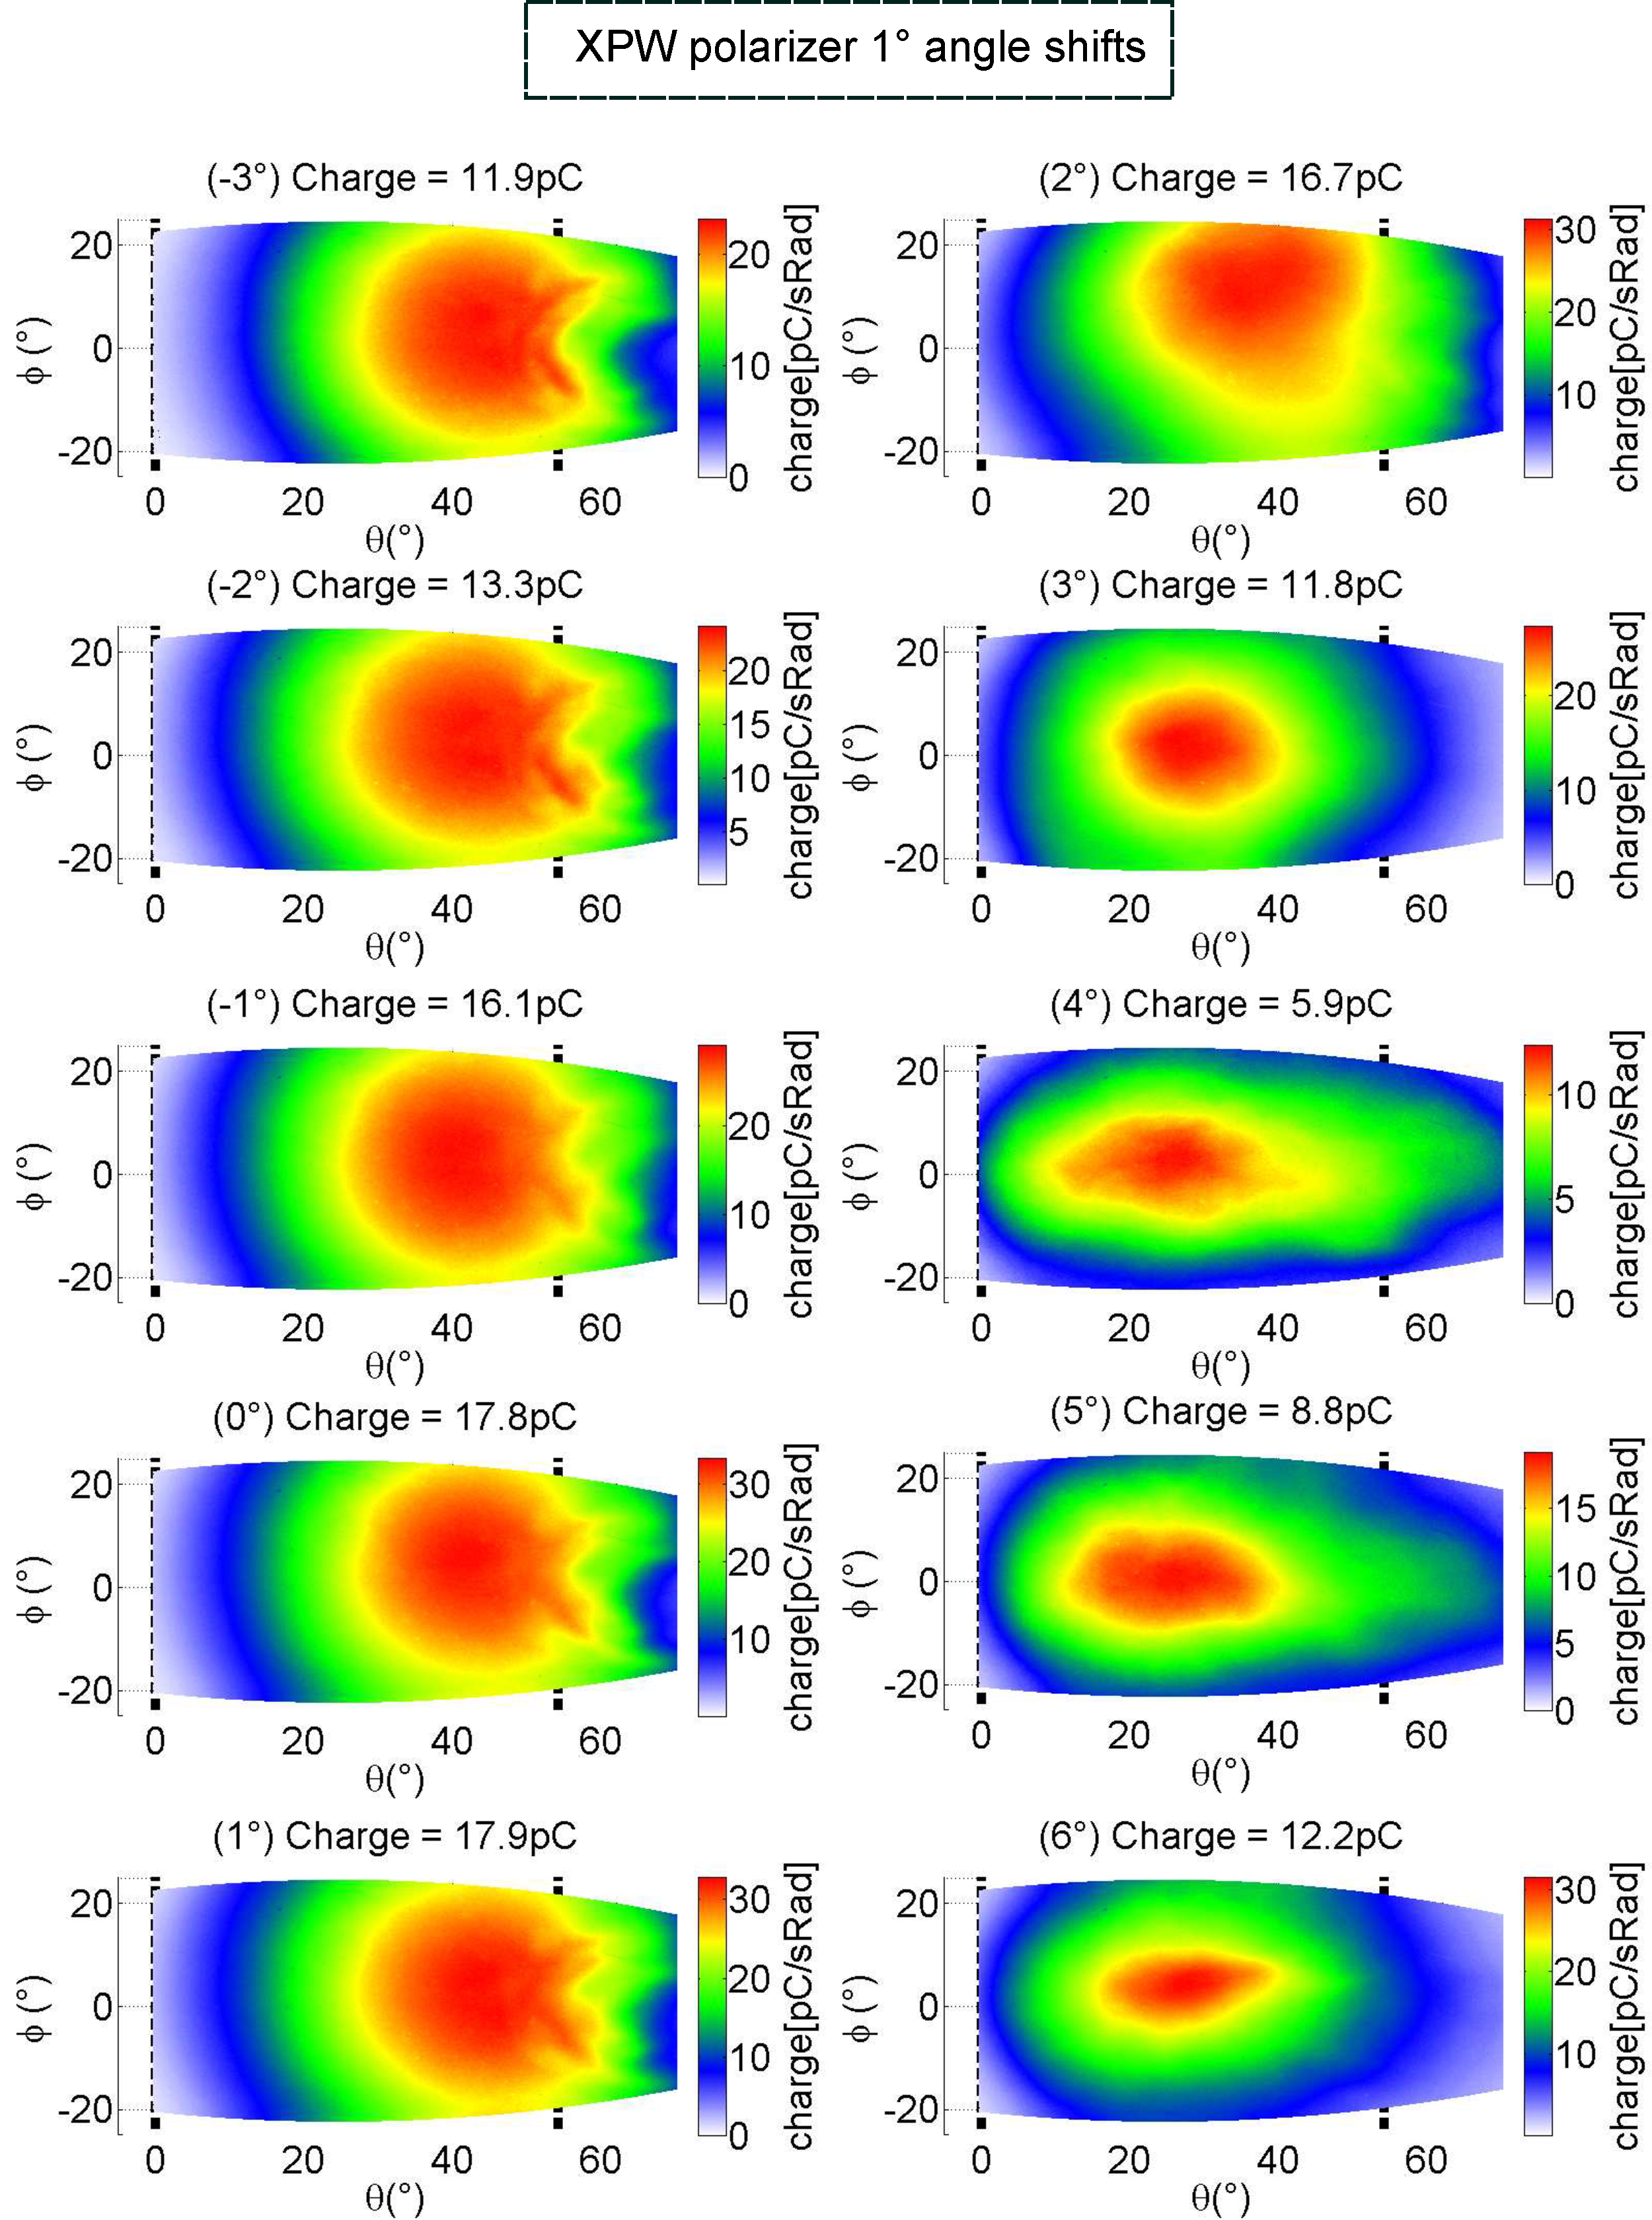
\includegraphics[width =\textwidth]{../chapitre4/images/XPW_29fs.pdf}\\
\caption{\label{fig:XPW_29fs}Influence of laser contrast on electron angular distribution. LANEX plane $\mathcal{L}: y = -0.51 x + 7.7\mathrm{(cm)}$. Both normal and specular directions are indicated by back dotted lines at respectively $0^{\circ}$ and $54^{\circ}$. Laser intensity is $a_0 = 0.6$, focal spot size $2.5\,\mathrm{\mu m}$ FWHM. }
\end{figure}


\begin{figure}[H]
\centering
\includegraphics[width =\textwidth]{../chapitre4/images/FocusDelay23fs_XPW279.pdf}\\
\caption{\label{fig:FocusDelay23fs_XPW279} Experimental electron angular distribution in the plane of laser polarization for an intensity on target $a_0 = 0.77$ for a waist of $\mathrm{2.5 \mu m}$ FWHM. Prepulse intensity is $I_p = 2\times 10^{14}\,\mathrm{W/cm^2}$}
\end{figure}



\subsection{Gyromagnetic confinement for short gradient scale length}\label{eq:Gyromagnetic confinement for short gradient scale lengths}

The present discussion is based only on the following experimental observation: for short plasma scale length, the optimal ejected charge does  not correspond to a laser in focus, where the peak intensity is maximal. 

\noindent The gyromagnetic effect, described in 2006~\cite{geindre2006relativistic}, could very well account for this experimental observation. The principle is that for relativistic intensities and very steep gradient density profiles, an imbalance between the $E$ and $B$ fields -- a ratio not like in an EM wave propagating in vacuum -- leads the magnetic force to confine electrons at the surface of the plasma, and these can no longer escape. This explains the drop in the amount of charge detected when the laser is in focus. Note that this observation requires a good laser contrast, and is different from the result presented in Fig~\ref{fig:20140808FocusScanElectronVShhgs}, where the contrast was voluntarily degraded. On the contrary there, the increase in plasma scale length limits electron ejection when the laser is in focus.

\noindent To evaluate the importance of this effect one should compare the cyclotron frequency $\omega_{ce}$ (Appendix~\ref{ch:Normalisation conventions}) to $\omega_{0}$, the laser frequency. For a p-polarized pulse reflecting on an ideal mirror as described in~\ref{subsection:Effet of interference field}:

$$
\frac{\omega_{ce}}{\omega_0} = a_0\frac{cB_{\parallel}}{E_{\perp}} = \frac{a_0}{\sin(\theta)} 
$$




\noindent where $\theta$ is the angle of incidence. This means that increasing $a_0$, or decreasing the incident angle, will also increase the cyclotron frequency. In our experimental conditions, this ratio is close to 1, since $a_0\sim 0.8$ and $\theta \sim 50^{\circ}$. The result of the laser focus z-scan is shown in Fig~\ref{fig:FocusScan} for a laser pulse of duration $30$fs (left column) and $23$fs (right column). We begin the scan at $\Delta z = 0$, which corresponds to the position of optimal charge ejected. The laser focuses after being reflected by the plasma mirror. When we progressively move the focus position closer to the target surface, that is to say for $\Delta z <0$, we observe a significant decrease in the total ejected charge, and note that a depletion line at $\phi = 0^{\circ}$ becomes visible in the spatial profile of the ejected electrons. We will explain the appearance of this depletion in section~\ref{sub:Influence of non axisymmetrical component of the interference field}.


\begin{figure}[H]
\centering
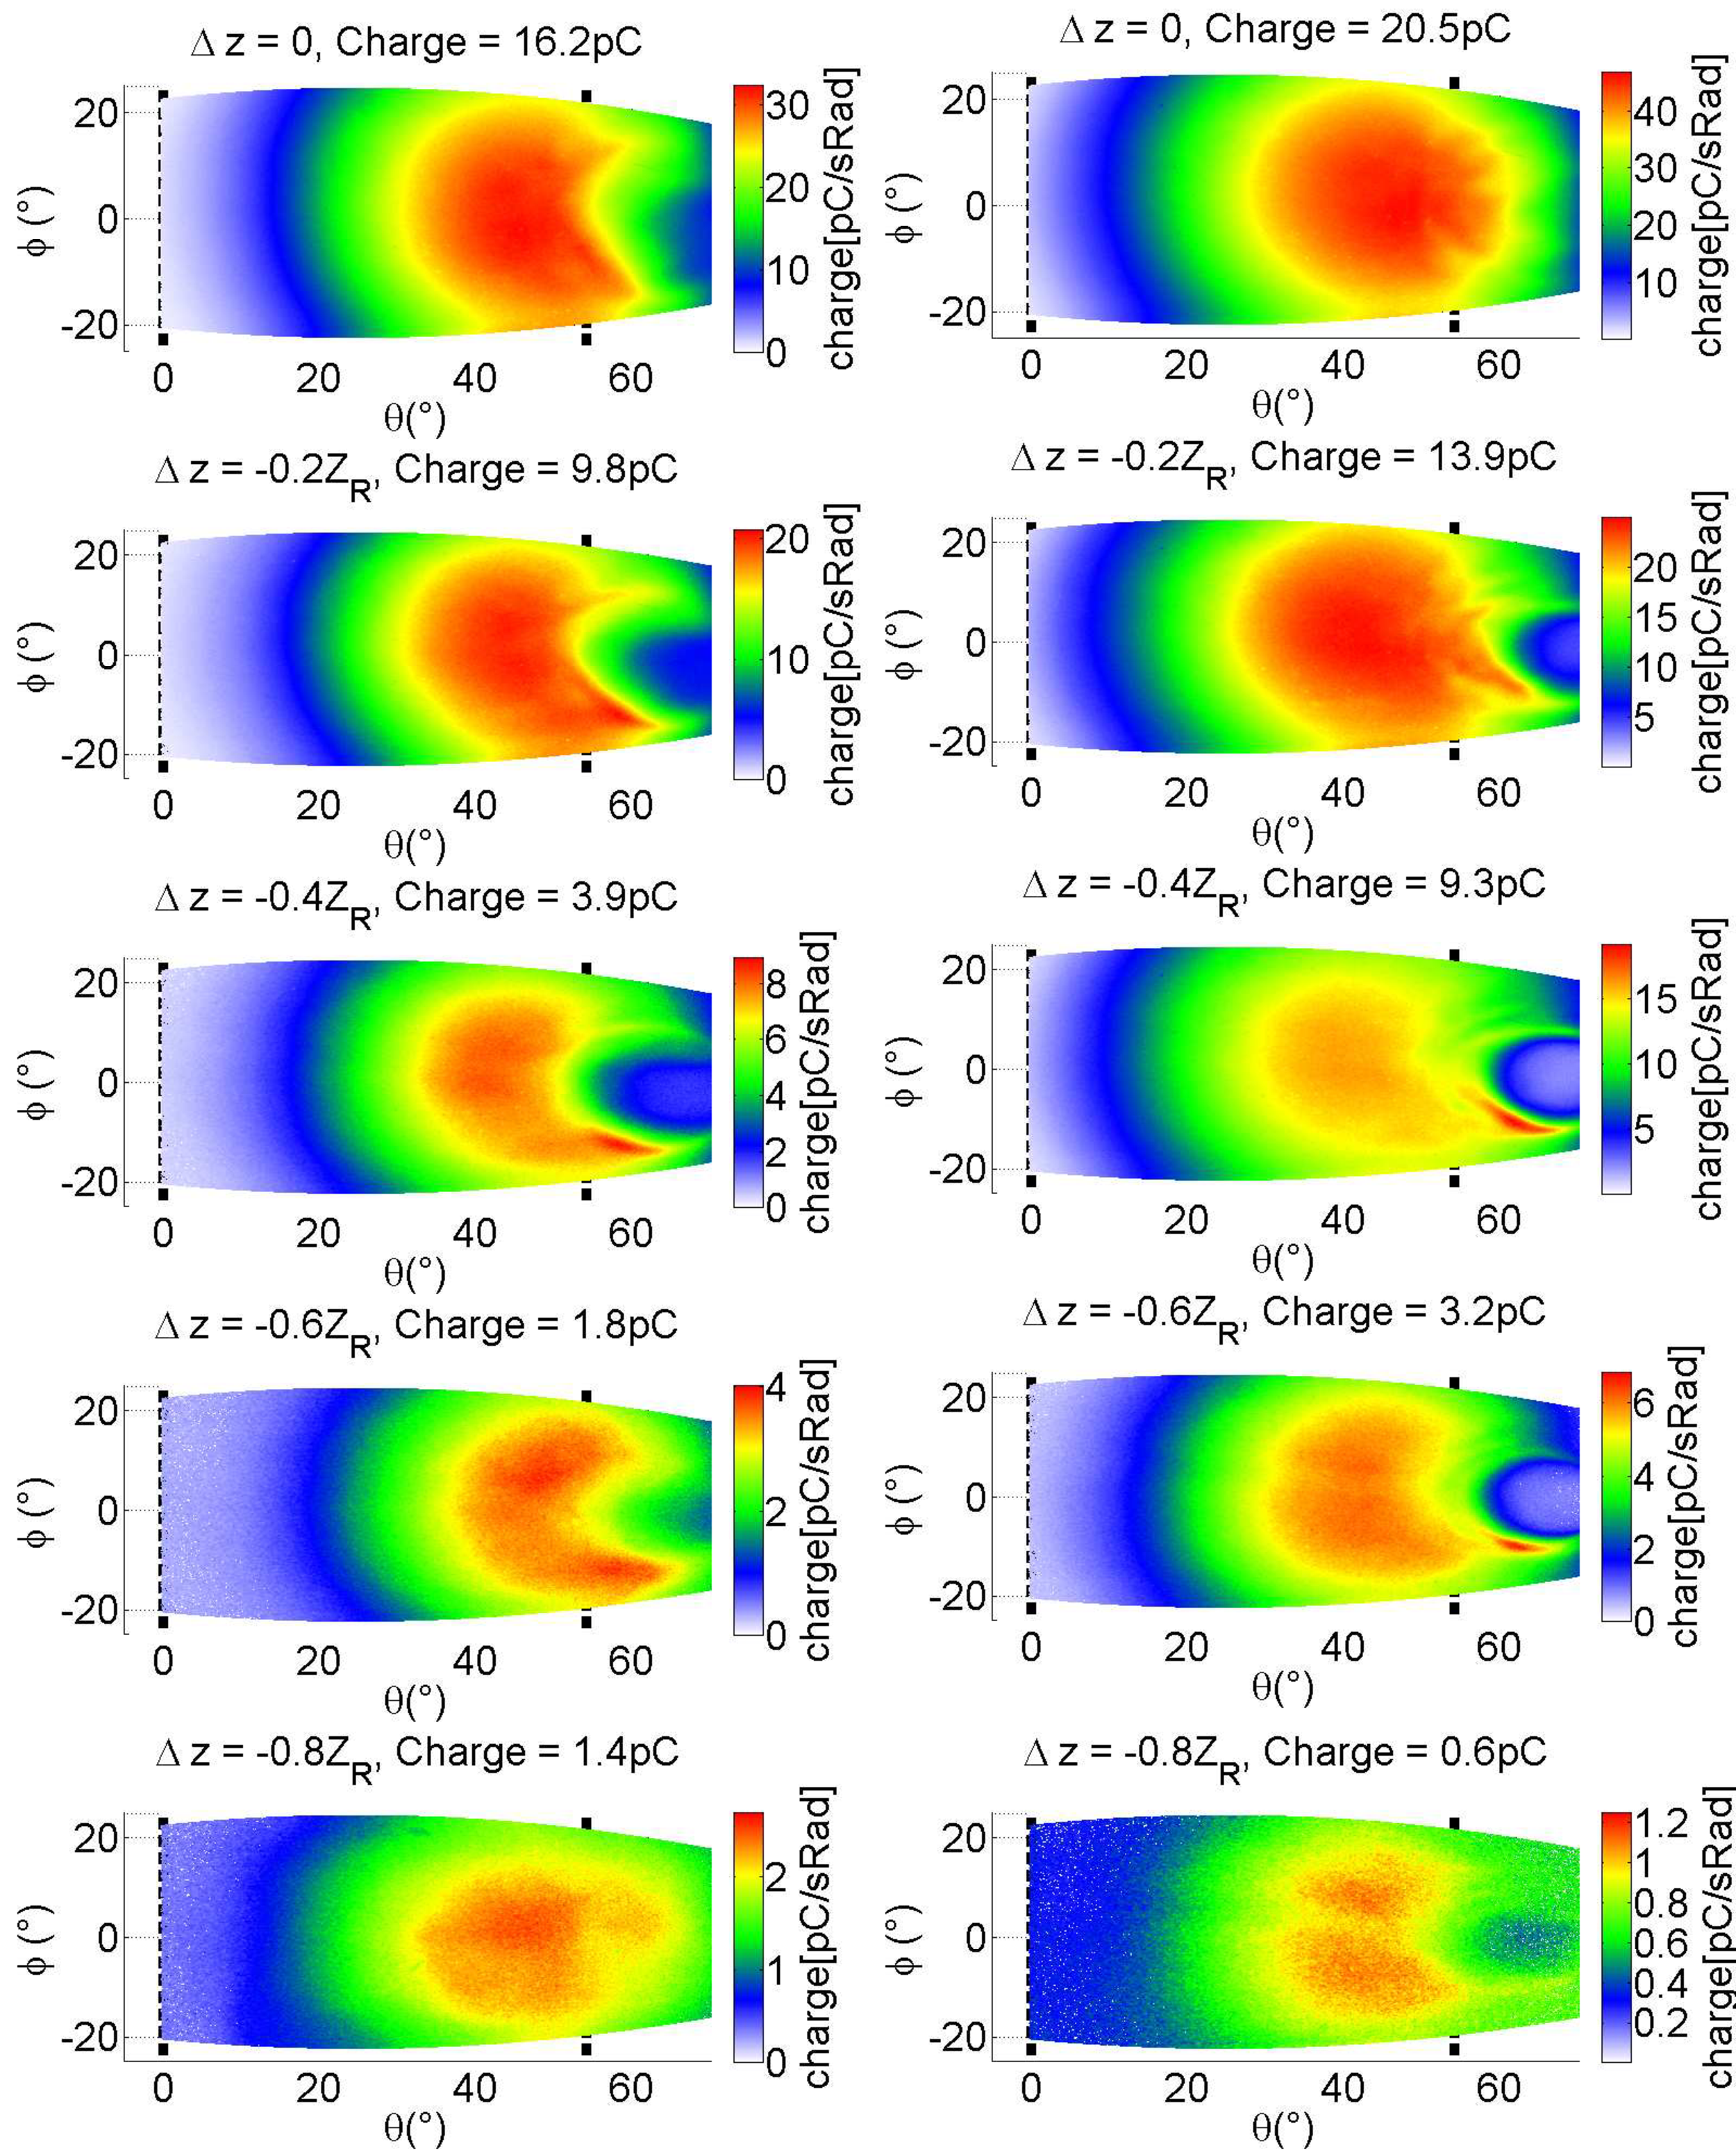
\includegraphics[width =\textwidth]{../chapitre4/images/FocusScan.pdf}\\
\caption{\label{fig:FocusScan}Laser focus z-scan $\Delta z$ while measuring the electron angular emission profile. The pulse duration is $30\,\mathrm{fs}$ with $a_0 = 0.6$ (the left column) and $23\,\mathrm{fs}$ with $a_0 \sim 0.7$ (rigth column). Laser focal spot size is $2.2\,\mathrm{\mu m}$ FWHM}
\end{figure}


%When proper conditions are met,  It appears that the electric field $E_z$ normal to the target show precisely this symmetry. We will reproduce this effect by injecting test electrons in a perfectely reflecting electromagnetic field using the experimental paramters, namely $w_0 = 2.2\mu m$, $a_0 = 0.7$.

%In focus, it was possible to observe a symmetry correponding to the interference field at the surface. In particular, this profile is shown in Fig~\ref{fig:focus-20-tir220-227} where the distribution is symetric with respect to the plane $\phi = 0^{\circ}$.
%
%\begin{figure}[H]
%\centering
%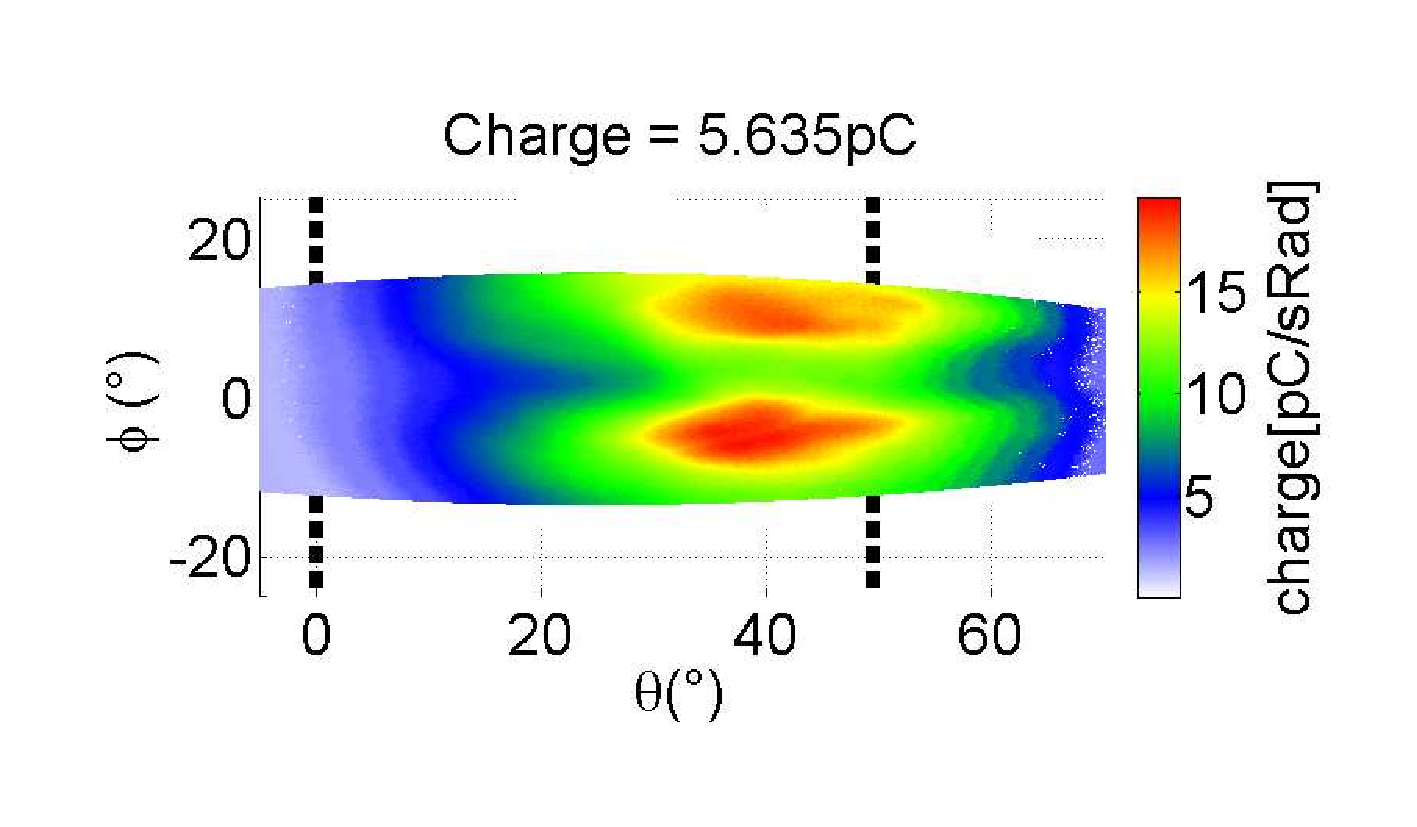
\includegraphics[width =\textwidth]{../chapitre4/images/focus-20-tir220-227.pdf}\\
%\caption{\label{fig:focus-20-tir220-227} Representative experimental electron distribution in the plane of laser polarization for an intensity on target $a_0 = 0.77$ and a focal spot of waist $w_0 = \mathrm{2.7 \mu m}$ }
%\end{figure}
%
%We will interpretate this result next section.







\section{Electron spectra}\label{subsub:Spectral measurement}

In order to measure the energy spectra of the electron ejected in our experiment, we removed the LANEX screen and replaced it with a purpose-built spectrometer. Here, we give details on the construction of this spectrometer and present experimental data. 

\subsection{Electron spectrometer}

The basic design is presented in Fig~\ref{fig:spectroSetup}(a) for the spectrometer normal to the target. It was mounted on a rotation stage centered on the focal spot such that we could rotate the angle of detection of the electrons. The entrance of the spectrometer is a $0.5\,\mathrm{mm}$ pinhole placed $100\,\mathrm{mm}$ from the focal spot. Neodymium magnets are inserted in the electron path and mounted on a vertical translation stage for proper calibration of the $0$ deviation position. The magnetic field along direction $y$ has been properly calibrated with a Hall probe along the line $(x,z) = (0,0)$ and the results is given in Fig~\ref{fig:spectroSetup}(b). Electrons are deviated in direction $z>0$ by the magnetic field and the trace is detected with a phosphor screen imaged with a CCD camera under vacuum.

\begin{figure}[H]
\centering
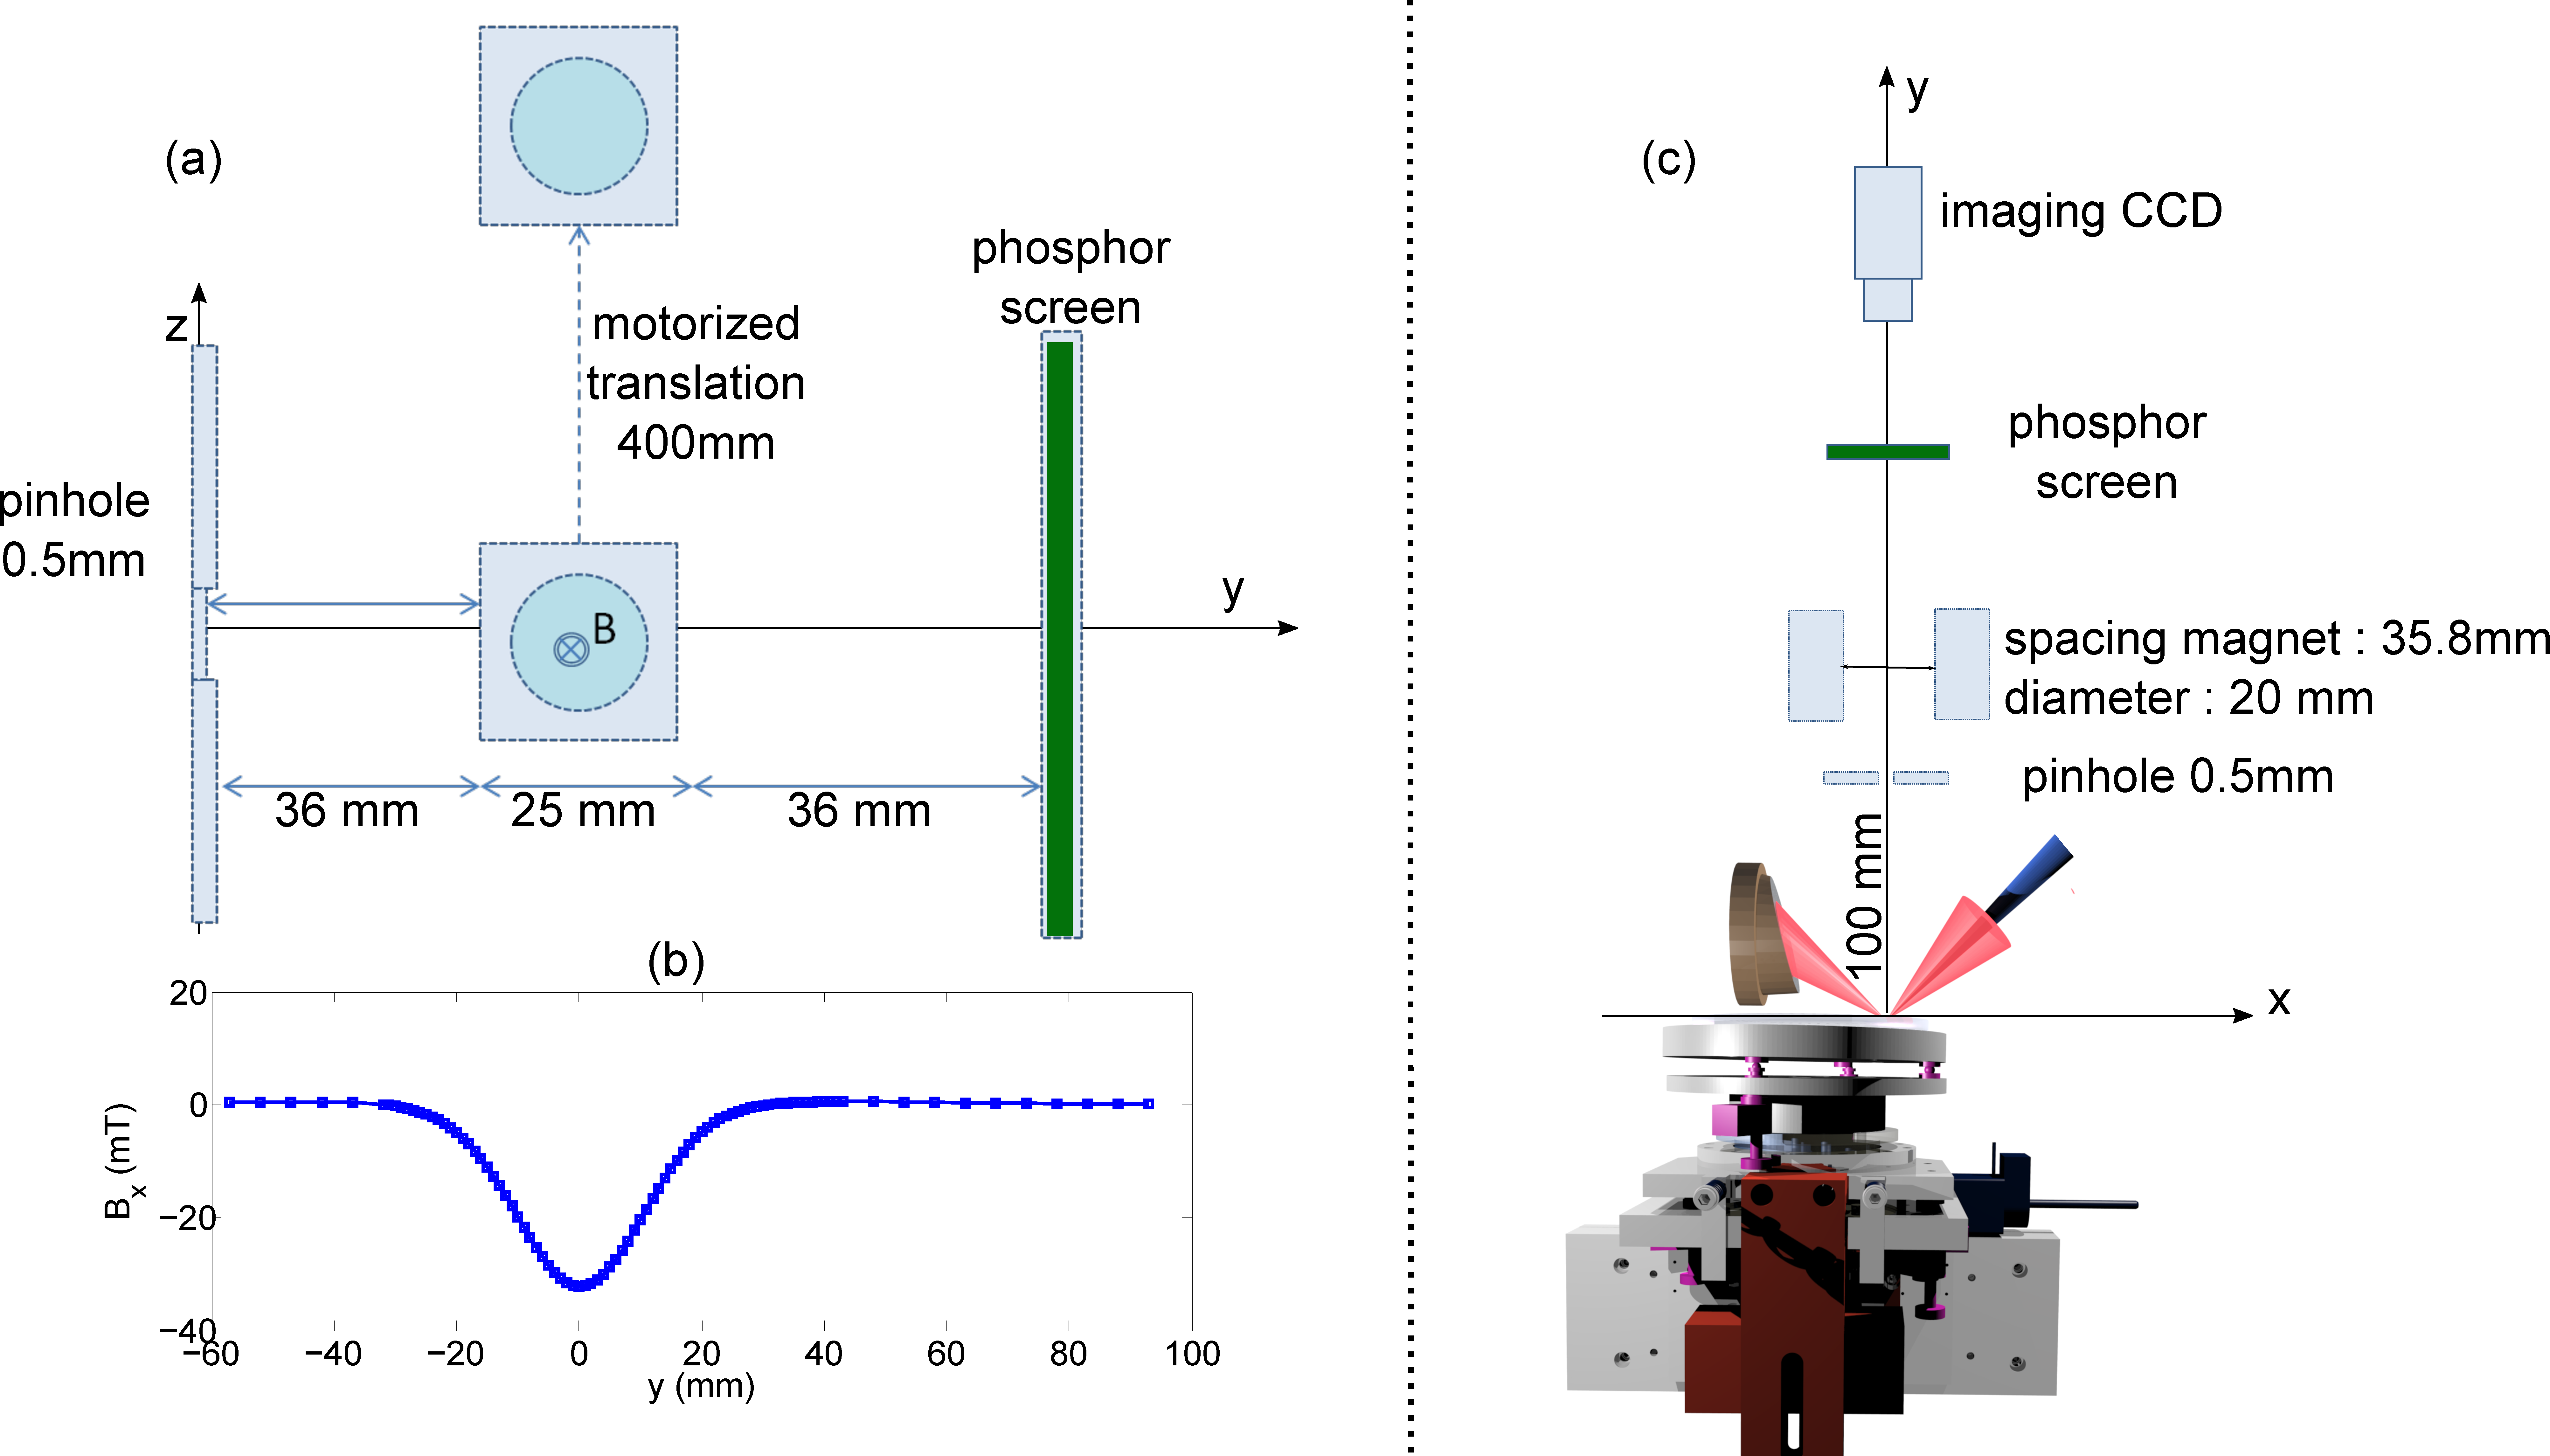
\includegraphics[width =\textwidth]{../chapitre4/images/spectroSetup.pdf}\\
\caption{\label{fig:spectroSetup} Electron spectrometer setup}
\end{figure}


\noindent To calibrate the detectable energy range in this configuration, we calculated the electron trajectories using the measured magnetic field map. Each final $z$ position of the electrons on the plane delimited by the phosphor therefore corresponds to a given kinetic energy. 


\subsection{Experimental results}

\noindent Deconvolved electron spectra are consistent with the scaling law provided by Eq~\ref{eq:ScaleLength}, since for $a_0 \sim 0.8$ and $L/\lambda \sim 0.1$, we expect electrons with energies of $\sim 300\,\mathrm{keV}$ .\\

\noindent \g{Influence of plasma gradient:}

\noindent Electrons are indeed accelerated to several hundreds of keV. In Fig~\ref{fig:tir257-228-238-20140804spectras-normalized}, we show the influence of the gradient scale length on the ejected electrons final energies. We observe that when the gradient is optimal (maximum signal on LANEX), the spectra extends up to 600keV. For short gradient scale length, that is to say in the absence of a prepulse, the spectrum peaks around 200keV. This indicates selective conditions for electrons to be efficiently accelerated, or in other words "trapped" in the reflected laser pulse. This is consistent with the previous observation that short gradient scale length can lead to highly collimated peaks in the global angular emission profile of electrons. We will discuss this further in Chapter~\ref{Laser-electron interaction in vacumm}.

\begin{figure}[H]
\centering
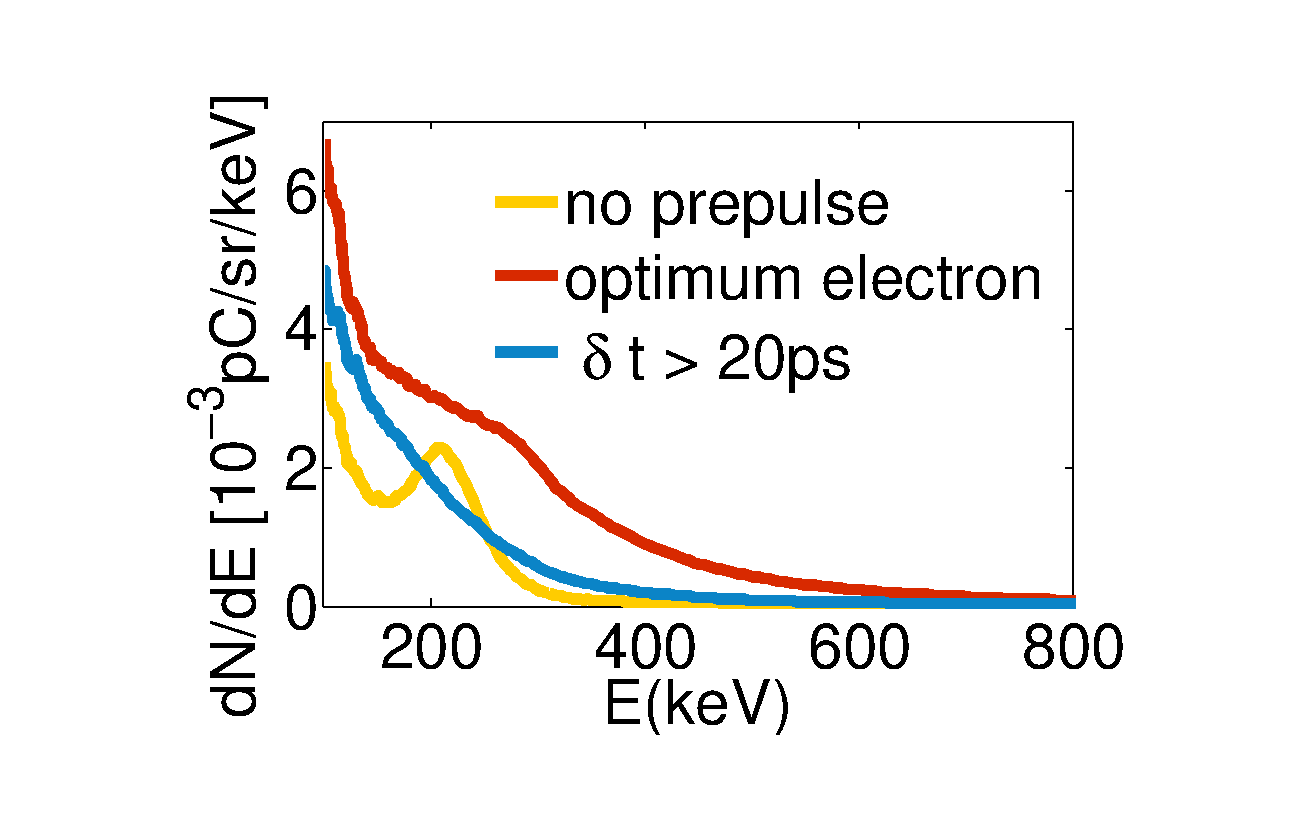
\includegraphics[width =0.7\textwidth]{../chapitre4/images/tir257-228-238-20140804spectras-normalized.pdf}\\
\caption{\label{fig:tir257-228-238-20140804spectras-normalized} Electron spectra normal to target. Signal is recorded when no prepulse is added, for a pump-probe delay $\delta t$ corresponding to an optimum on the LANEX, and for long pump/probe delays}
\end{figure}

\noindent \g{Influence of angle to normal:}

\noindent We do not observe significant differences in the electron energy spectra depending on the emission angle to the target from $0$ to $40^{\circ}$. In Fig~\ref{fig:20140408ScanAngleSpectresTIRS102-118-error0p05-secondrun}, a prepulse of $3\times 10^{14}\,\mathrm{W/cm^2}$ preionizes the target at a pump-probe delay of $6\,\mathrm{ps}$ before the interaction. We find that electrons are accelerated up to several hundreds of keV. 

\begin{figure}[H]
\centering
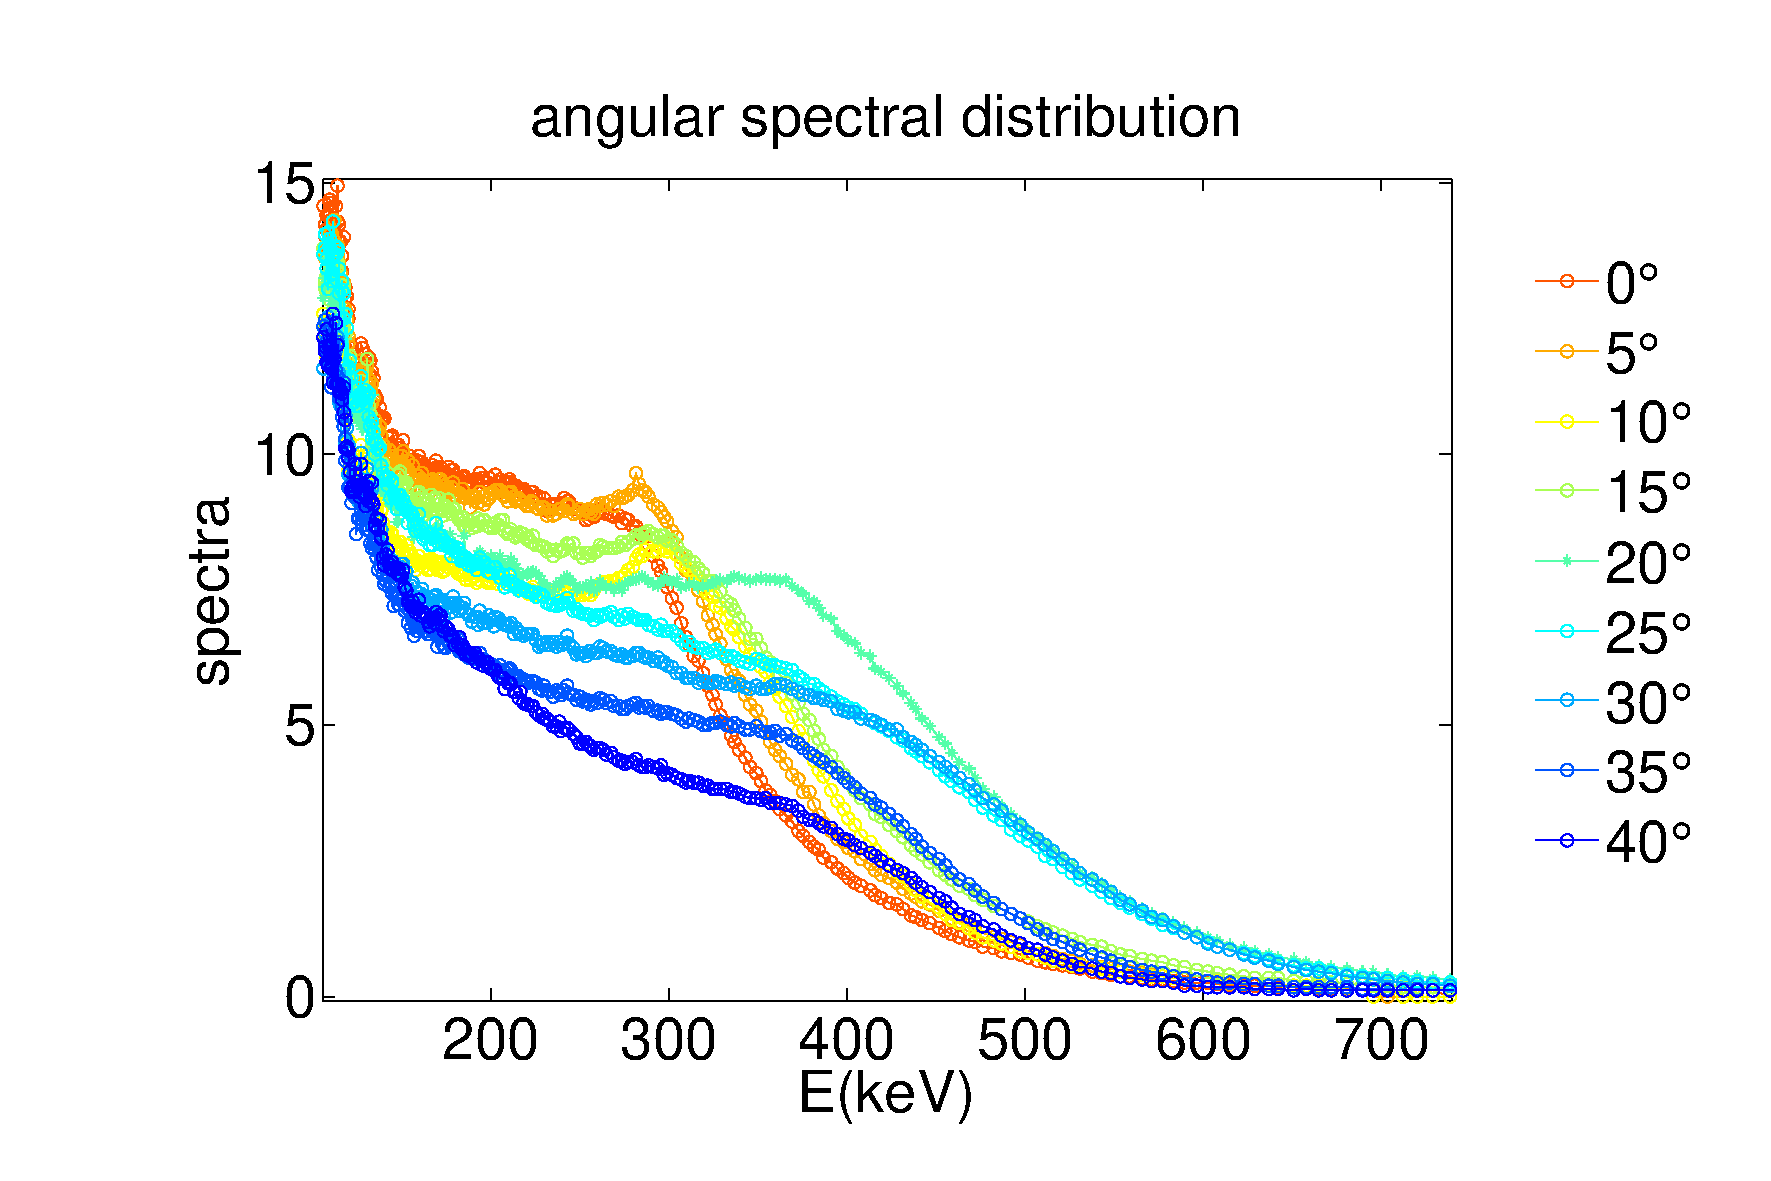
\includegraphics[width =0.9\textwidth]{../chapitre4/images/20140408ScanAngleSpectresTIRS102-118-error0p05-secondrun.pdf}\\
\caption{\label{fig:20140408ScanAngleSpectresTIRS102-118-error0p05-secondrun} Electron spectra for various angles $\theta \in [0^{\circ} \ \ 40^{\circ}]$. $a_0 = 0.7$, $L/\lambda \sim 0.1$. Pump/probe delay is $6\,\mathrm{ps}$ with a prepulse intensity of $3\times 10^{14}\,\mathrm{W/cm^2}$  }
\end{figure}





\section{Conclusion}

We have demonstrated that in the sub-relativistic regime, the electron and harmonic emission from plasma mirrors have opposite dependence on the plasma scale length. Harmonic emission requires very short plasma scale length $<0.06\lambda$ for $a_0\sim 0.8$ while electron emission becomes efficient once the plasma has expanded. This behavior was successfully reproduced by 2D PIC simulations, and the increase of ejected charge attributed to the effect of space charge field creating on the surface of the plasma. When this emission is optimal, electron acceleration is the most efficient and reaches several hundreds of keV as expected by simple scaling laws. In addition, the presence of a ponderomotive hole in the electron emission angular profile, where no peaks of emission can be seen, shows that electrons are not "trapped" inside the laser but rather gain most of their energy in the plasma before being ejected.










%\subsection{Dispersion of an electron bunch}
%
%With the emmergence of femtosecond and attosecond physics, several experimental teams have been trying to generate short ($<fs$) electron bunches. 
%One interesting application is for example time resvoled diffraction of dense crystalline solids through pump-probe experimental schemes. 
%
%If we consider a spacial bunch of electrons with arbitrary velocity, we quickly reach the conclusion that the bunch will undergo a coulomb explosion because of the self-induced repulsive electromagnetic field. 



%
%\begin{figure}[H]
%\centering
%\fbox{\includegraphics[width =15cm]{../chapitre4/images/ElectronProfilWithDelay.pdf}}\\
%\caption{\label{fig:ElectronProfilWithDelay} Representative experimental electron distribution in the plane of laser polarization for an intensity on target $I = 1.26 \times 10^{18}\,\mathrm{W/cm}^2$ ($a_0 = 0.77$)and a focal spot of $2.7 \mathrm{\mu m}$ at FWHM and $I_{prepulse} = 1.24 10^{15}\,\mathrm{W/cm}^2$ of $15.2  \mathrm{\mu m}$ et FWHM}
%\end{figure}
%
%This depletion line observe can be due to a strong laser/electron beam coupling or to a degradation of the laser spatial phase because we used a cone to filter out the laser instead of a hollow core fiber. 


%\begin{figure}[!h]
%\centering
%\fbox{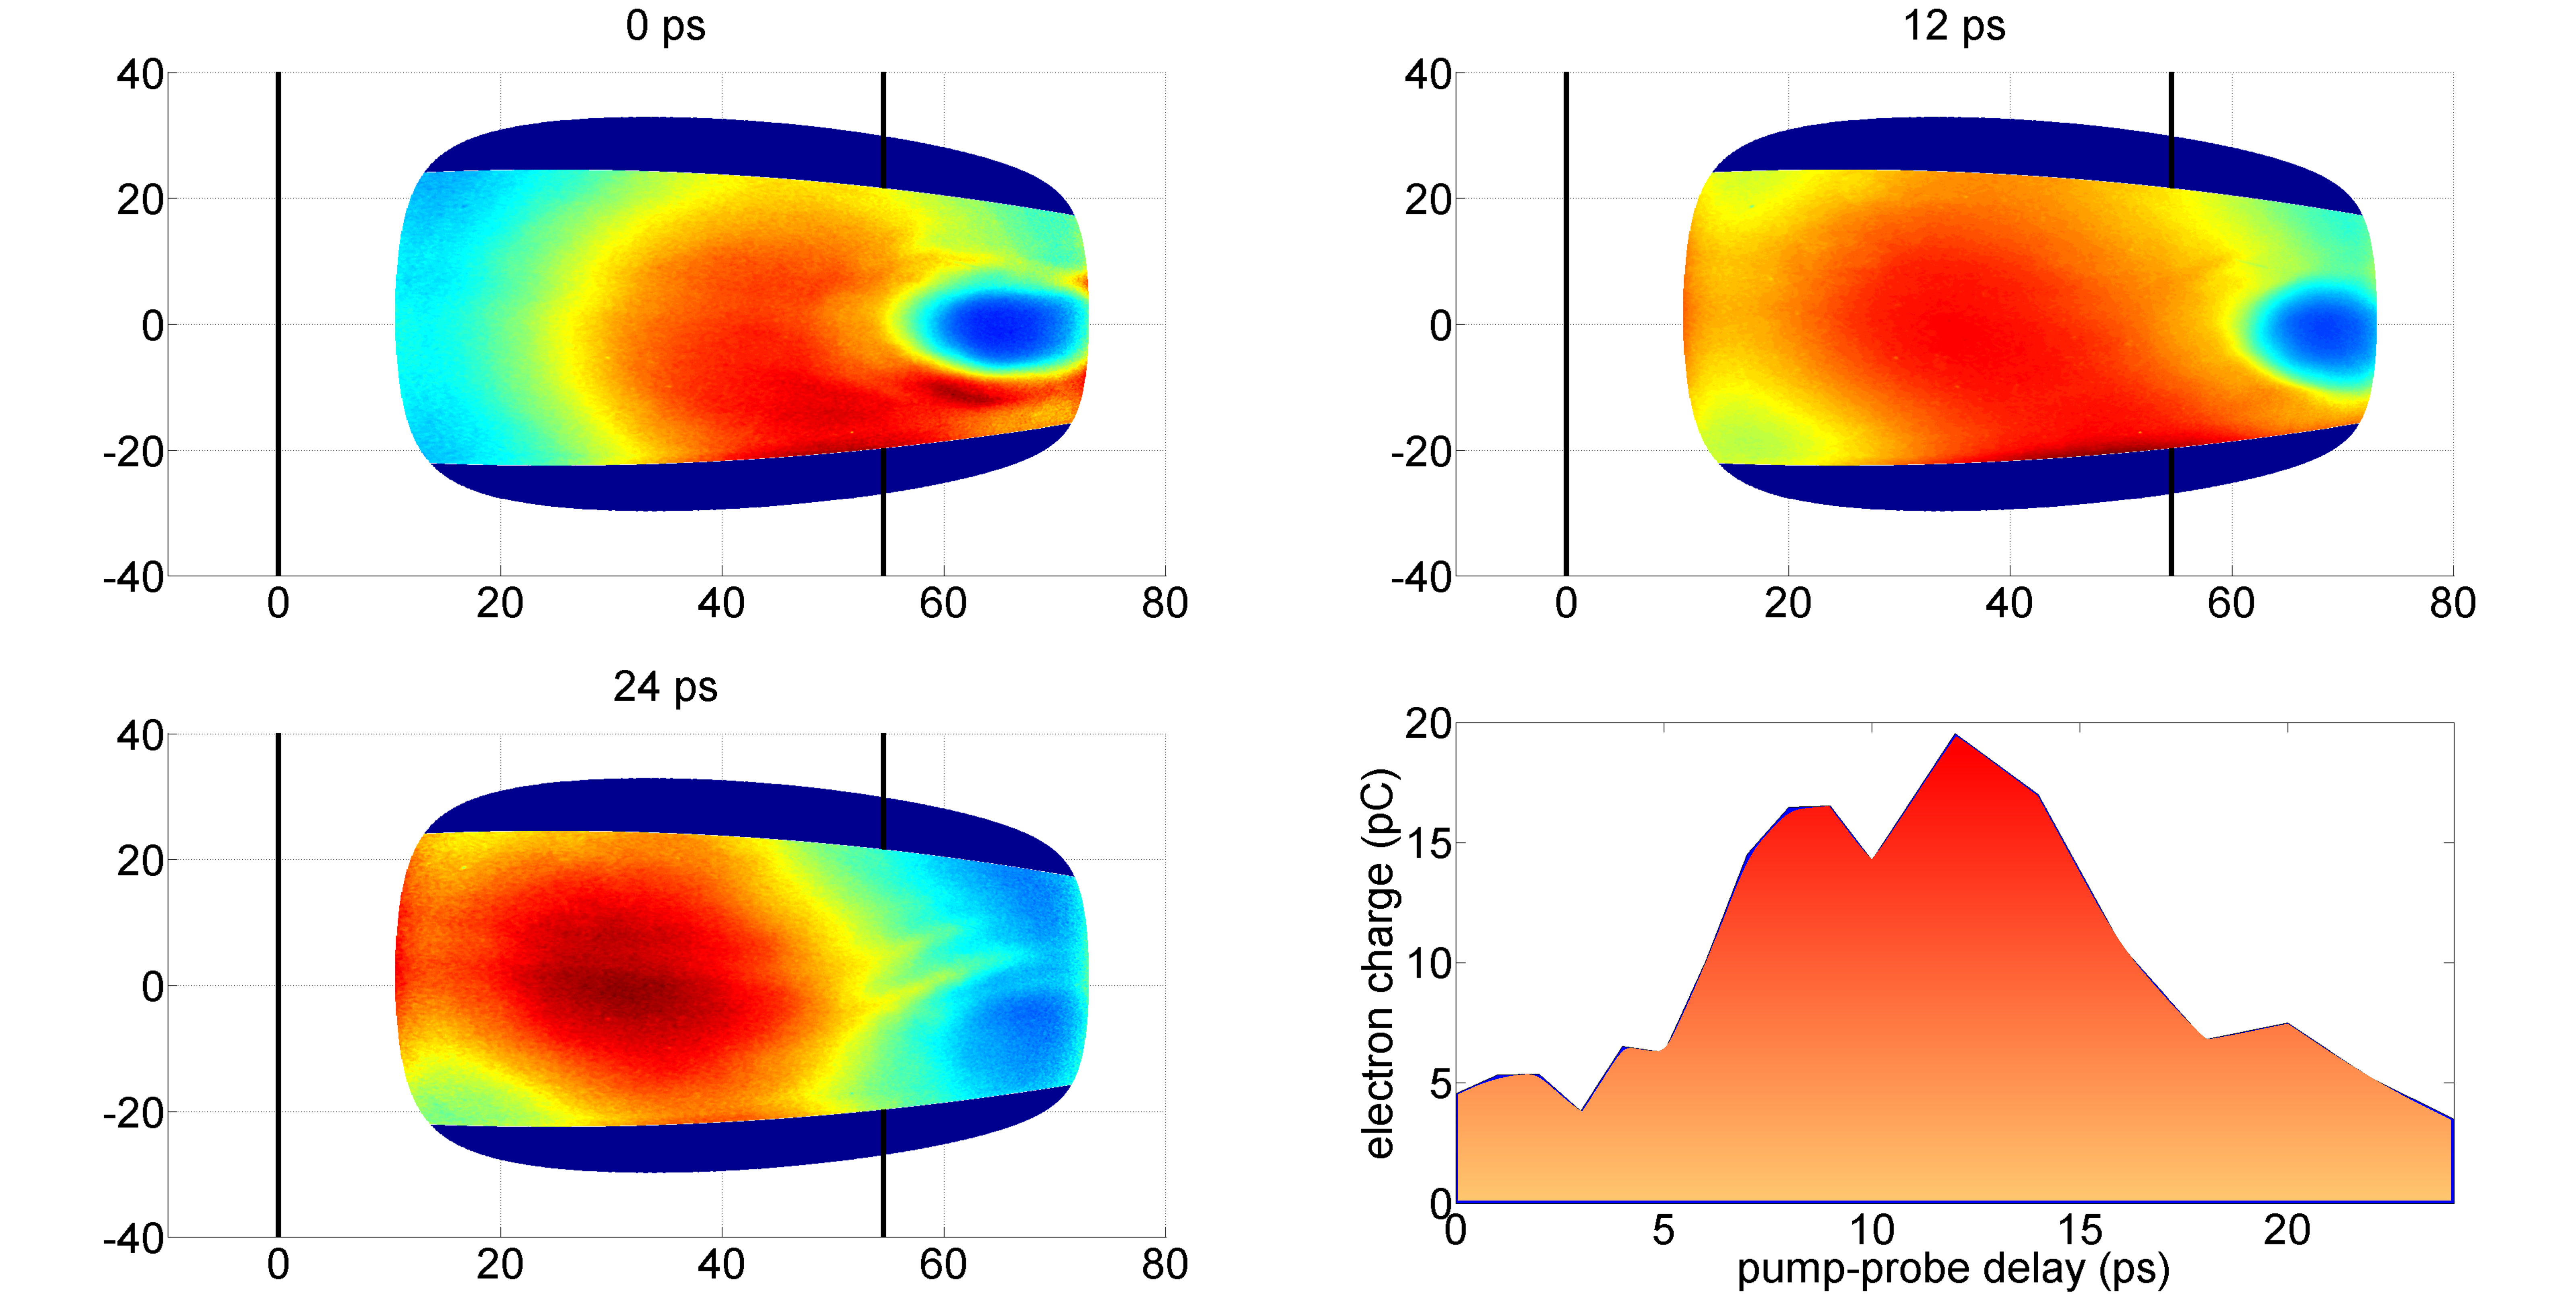
\includegraphics[width =13cm]{../chapitre4/images/08092014-trou.pdf}}\\
%\caption{\label{fig:08092014-trou}series du 08/09/2014 $\theta_{inc} = 54.5$deg, tirs 297-315}
%\end{figure}





















































